% ============================================================
%  MONOGRAFÍA — UNIVERSIDAD MAYOR DE SAN SIMÓN
%  Facultad de Ciencias y Tecnología — Dirección de Posgrado
%  Diplomado en Ciencia de Datos
%  ------------------------------------------------------------
%  COMPILACIÓN (IMPORTANTE):
%     lualatex main.tex      <- recomendado
%     lualatex main.tex      <- segunda pasada: resuelve índices
%                               y referencias cruzadas
%  (XeLaTeX también funciona: xelatex main.tex, dos veces.)
%
%  NO usar pdflatex: este documento carga fuentes del sistema
%  (Arial / Garamond) vía fontspec, lo cual pdflatex no soporta.
%  Ver README.md para el detalle.
% ============================================================

%  PANEL DE CONTROL: datos del proyecto e interruptores.
%  Va ANTES del preámbulo porque el formato reacciona a los
%  interruptores (folio, numeración, color, tipografía).
% ============================================================
%  PANEL DE CONTROL — configuracion.tex
%  ------------------------------------------------------------
%  TODO lo que cambia de una versión a otra vive AQUÍ. Ni
%  main.tex ni los archivos de secciones/ llevan datos ni
%  interruptores de formato.
%
%  Uso:  main.tex empieza con  % ============================================================
%  PANEL DE CONTROL — configuracion.tex
%  ------------------------------------------------------------
%  TODO lo que cambia de una versión a otra vive AQUÍ. Ni
%  main.tex ni los archivos de secciones/ llevan datos ni
%  interruptores de formato.
%
%  Uso:  main.tex empieza con  % ============================================================
%  PANEL DE CONTROL — configuracion.tex
%  ------------------------------------------------------------
%  TODO lo que cambia de una versión a otra vive AQUÍ. Ni
%  main.tex ni los archivos de secciones/ llevan datos ni
%  interruptores de formato.
%
%  Uso:  main.tex empieza con  \input{configuracion.tex}
%        (antes del preámbulo, para que este pueda reaccionar a
%        los interruptores) y después entra el contenido.
% ============================================================

% ============================================================
%  1. DATOS DEL PROYECTO
% ============================================================

% ---------- Título de la monografía ------------------------
% El título se imprime en MAYÚSCULAS, Arial 20 negrita, centrado
% y con los saltos de línea ESCRITOS A MANO: la guía no permite
% reducir el tamaño de la fuente, así que la pirámide invertida
% se consigue cortando el título en renglones explícitos.
% El bloque útil mide 16,09 cm; a Arial 20 negrita el renglón más
% ancho que puede empezar por "IDENTIFICACIÓN" mide 11,8 cm
% (la palabra siguiente ya no cabe), de modo que la pirámide
% necesariamente tiene su base en los renglones 2 y 3 y se
% estrecha hacia abajo, que es la silueta del modelo.
% Anchuras de los renglones, de arriba abajo:
%   11,8 · 15,8 · 15,3 · 12,0 · 12,6 · 3,8 cm
% Para cambiar el corte basta reescribir estas líneas: si un
% renglón no cabe en 16,09 cm se partirá en dos (y la pirámide se
% pierde), así que conviene medir el resultado con
% "scripts/verificar" tras cada ajuste.

% Interruptor: modo borrador con figuras pendientes visibles (true)
% o modo entrega sin recuadros (false). Ver preambulo.tex sección 12.
\newif\ifborrador
\borradortrue  % default: muestra recuadros de "Figura pendiente"
\newcommand{\tituloLineaA}{Estimación del número esperado de}
\newcommand{\tituloLineaB}{consultas de ruta de Trufi App por}
\newcommand{\tituloLineaC}{celda H3 en el eje metropolitano}
\newcommand{\tituloLineaD}{de Cochabamba mediante técnicas}
\newcommand{\tituloLineaE}{geoespaciales de Ciencia de Datos}
\newcommand{\tituloMonografia}{%
  \tituloLineaA\\
  \tituloLineaB\\
  \tituloLineaC\\
  \tituloLineaD\\
  \tituloLineaE}
% Versión en una sola línea, solo para los metadatos del PDF
% (\hypersetup no admite saltos de línea).
\newcommand{\tituloMonografiaPlano}{Estimación del número esperado de consultas de ruta
  de Trufi App por celda H3 en el eje metropolitano de Cochabamba mediante técnicas
  geoespaciales de Ciencia de Datos}
% Título corto: el del encabezado corrido del cuerpo (Fase 5).
\newcommand{\tituloCorto}{Demanda esperada de consultas de Trufi App por celda H3}

% ---------- Postulante, programa, versión y año --------------
\newcommand{\nombreDiplomado}{Ciencia de Datos}
\newcommand{\nombreVersion}{CUARTA}
\newcommand{\nombrePostulante}{José Roberto Vargas Orellana}
\newcommand{\anioMonografia}{2026}
\newcommand{\ciudadMonografia}{Cochabamba -- Bolivia}

% ---------- Docente y módulo (línea oculta por defecto) -----
% La guía los menciona en §2 pero no aparecen en el modelo de
% la carátula, así que quedan ocultos. Para mostrarlos basta
% poner \mostrarDocentetrue más abajo.
\newcommand{\nombreDocente}{Nombre del docente}
\newcommand{\nombreModulo}{Nombre del módulo}

% ============================================================
%  2. INTERRUPTORES
% ------------------------------------------------------------
%  El valor por defecto de cada línea es el de la guía; la
%  alternativa se consigue cambiando solo el "true"/"false".
% ============================================================

% ---------- Numeración de páginas ---------------------------
%   false (guía)  = romanos en los preliminares + arábigos desde 1
%   true  (modelo)= arábiga continua desde la carátula
\newif\ifnumeracionContinua
\numeracionContinuafalse

% ---------- Posición del folio ------------------------------
%   false = abajo y centrado (lo exige la guía)
%   true  = abajo a la derecha
\newif\iffolioDerecha
\folioDerechafalse

% ---------- Línea docente/módulo en la carátula --------------
%   false = oculta · true = visible
\newif\ifmostrarDocente
\mostrarDocentefalse

% ---------- Modo del documento ------------------------------
%   false = final      (falla la compilación si quedan marcadores)
%   true  = borrador   (resalta los marcadores de trabajo)
\newif\ifmodoBorrador
\modoBorradorfalse

% ---------- Color ------------------------------------------
%   true  = digital, con el azul marino de acento
%   false = impresión, todo en negro y gris
\newif\ifcolorDigital
\colorDigitaltrue

% ---------- Preliminares opcionales ------------------------
%   true  = mostrar dedicatoria, agradecimientos, glosario e
%           índices de tablas y figuras si existen
%   false = ocultarlos
\newif\ifmostrarOpcionales
\mostrarOpcionalestrue

% ---------- Compilar un solo capítulo ----------------------
%   false = documento completo
%   true  = solo el capítulo indicado en \capituloUnico
%           (útil para escribir una sección sin recompilar todo)
\newif\ifcompilarUnCapitulo
\compilarUnCapitulofalse
\newcommand{\capituloUnico}{08_desarrollo}

% ---------- Estilo de bibliografía -------------------------
%   false = APA: alfabética, sin numerar (predeterminado)
%   true  = numerada, formato de la guía §3.6
\newif\ifbibNumerada
\bibNumeradafalse

%        (antes del preámbulo, para que este pueda reaccionar a
%        los interruptores) y después entra el contenido.
% ============================================================

% ============================================================
%  1. DATOS DEL PROYECTO
% ============================================================

% ---------- Título de la monografía ------------------------
% El título se imprime en MAYÚSCULAS, Arial 20 negrita, centrado
% y con los saltos de línea ESCRITOS A MANO: la guía no permite
% reducir el tamaño de la fuente, así que la pirámide invertida
% se consigue cortando el título en renglones explícitos.
% El bloque útil mide 16,09 cm; a Arial 20 negrita el renglón más
% ancho que puede empezar por "IDENTIFICACIÓN" mide 11,8 cm
% (la palabra siguiente ya no cabe), de modo que la pirámide
% necesariamente tiene su base en los renglones 2 y 3 y se
% estrecha hacia abajo, que es la silueta del modelo.
% Anchuras de los renglones, de arriba abajo:
%   11,8 · 15,8 · 15,3 · 12,0 · 12,6 · 3,8 cm
% Para cambiar el corte basta reescribir estas líneas: si un
% renglón no cabe en 16,09 cm se partirá en dos (y la pirámide se
% pierde), así que conviene medir el resultado con
% "scripts/verificar" tras cada ajuste.

% Interruptor: modo borrador con figuras pendientes visibles (true)
% o modo entrega sin recuadros (false). Ver preambulo.tex sección 12.
\newif\ifborrador
\borradortrue  % default: muestra recuadros de "Figura pendiente"
\newcommand{\tituloLineaA}{Estimación del número esperado de}
\newcommand{\tituloLineaB}{consultas de ruta de Trufi App por}
\newcommand{\tituloLineaC}{celda H3 en el eje metropolitano}
\newcommand{\tituloLineaD}{de Cochabamba mediante técnicas}
\newcommand{\tituloLineaE}{geoespaciales de Ciencia de Datos}
\newcommand{\tituloMonografia}{%
  \tituloLineaA\\
  \tituloLineaB\\
  \tituloLineaC\\
  \tituloLineaD\\
  \tituloLineaE}
% Versión en una sola línea, solo para los metadatos del PDF
% (\hypersetup no admite saltos de línea).
\newcommand{\tituloMonografiaPlano}{Estimación del número esperado de consultas de ruta
  de Trufi App por celda H3 en el eje metropolitano de Cochabamba mediante técnicas
  geoespaciales de Ciencia de Datos}
% Título corto: el del encabezado corrido del cuerpo (Fase 5).
\newcommand{\tituloCorto}{Demanda esperada de consultas de Trufi App por celda H3}

% ---------- Postulante, programa, versión y año --------------
\newcommand{\nombreDiplomado}{Ciencia de Datos}
\newcommand{\nombreVersion}{CUARTA}
\newcommand{\nombrePostulante}{José Roberto Vargas Orellana}
\newcommand{\anioMonografia}{2026}
\newcommand{\ciudadMonografia}{Cochabamba -- Bolivia}

% ---------- Docente y módulo (línea oculta por defecto) -----
% La guía los menciona en §2 pero no aparecen en el modelo de
% la carátula, así que quedan ocultos. Para mostrarlos basta
% poner \mostrarDocentetrue más abajo.
\newcommand{\nombreDocente}{Nombre del docente}
\newcommand{\nombreModulo}{Nombre del módulo}

% ============================================================
%  2. INTERRUPTORES
% ------------------------------------------------------------
%  El valor por defecto de cada línea es el de la guía; la
%  alternativa se consigue cambiando solo el "true"/"false".
% ============================================================

% ---------- Numeración de páginas ---------------------------
%   false (guía)  = romanos en los preliminares + arábigos desde 1
%   true  (modelo)= arábiga continua desde la carátula
\newif\ifnumeracionContinua
\numeracionContinuafalse

% ---------- Posición del folio ------------------------------
%   false = abajo y centrado (lo exige la guía)
%   true  = abajo a la derecha
\newif\iffolioDerecha
\folioDerechafalse

% ---------- Línea docente/módulo en la carátula --------------
%   false = oculta · true = visible
\newif\ifmostrarDocente
\mostrarDocentefalse

% ---------- Modo del documento ------------------------------
%   false = final      (falla la compilación si quedan marcadores)
%   true  = borrador   (resalta los marcadores de trabajo)
\newif\ifmodoBorrador
\modoBorradorfalse

% ---------- Color ------------------------------------------
%   true  = digital, con el azul marino de acento
%   false = impresión, todo en negro y gris
\newif\ifcolorDigital
\colorDigitaltrue

% ---------- Preliminares opcionales ------------------------
%   true  = mostrar dedicatoria, agradecimientos, glosario e
%           índices de tablas y figuras si existen
%   false = ocultarlos
\newif\ifmostrarOpcionales
\mostrarOpcionalestrue

% ---------- Compilar un solo capítulo ----------------------
%   false = documento completo
%   true  = solo el capítulo indicado en \capituloUnico
%           (útil para escribir una sección sin recompilar todo)
\newif\ifcompilarUnCapitulo
\compilarUnCapitulofalse
\newcommand{\capituloUnico}{08_desarrollo}

% ---------- Estilo de bibliografía -------------------------
%   false = APA: alfabética, sin numerar (predeterminado)
%   true  = numerada, formato de la guía §3.6
\newif\ifbibNumerada
\bibNumeradafalse

%        (antes del preámbulo, para que este pueda reaccionar a
%        los interruptores) y después entra el contenido.
% ============================================================

% ============================================================
%  1. DATOS DEL PROYECTO
% ============================================================

% ---------- Título de la monografía ------------------------
% El título se imprime en MAYÚSCULAS, Arial 20 negrita, centrado
% y con los saltos de línea ESCRITOS A MANO: la guía no permite
% reducir el tamaño de la fuente, así que la pirámide invertida
% se consigue cortando el título en renglones explícitos.
% El bloque útil mide 16,09 cm; a Arial 20 negrita el renglón más
% ancho que puede empezar por "IDENTIFICACIÓN" mide 11,8 cm
% (la palabra siguiente ya no cabe), de modo que la pirámide
% necesariamente tiene su base en los renglones 2 y 3 y se
% estrecha hacia abajo, que es la silueta del modelo.
% Anchuras de los renglones, de arriba abajo:
%   11,8 · 15,8 · 15,3 · 12,0 · 12,6 · 3,8 cm
% Para cambiar el corte basta reescribir estas líneas: si un
% renglón no cabe en 16,09 cm se partirá en dos (y la pirámide se
% pierde), así que conviene medir el resultado con
% "scripts/verificar" tras cada ajuste.

% Interruptor: modo borrador con figuras pendientes visibles (true)
% o modo entrega sin recuadros (false). Ver preambulo.tex sección 12.
\newif\ifborrador
\borradortrue  % default: muestra recuadros de "Figura pendiente"
\newcommand{\tituloLineaA}{Estimación del número esperado de}
\newcommand{\tituloLineaB}{consultas de ruta de Trufi App por}
\newcommand{\tituloLineaC}{celda H3 en el eje metropolitano}
\newcommand{\tituloLineaD}{de Cochabamba mediante técnicas}
\newcommand{\tituloLineaE}{geoespaciales de Ciencia de Datos}
\newcommand{\tituloMonografia}{%
  \tituloLineaA\\
  \tituloLineaB\\
  \tituloLineaC\\
  \tituloLineaD\\
  \tituloLineaE}
% Versión en una sola línea, solo para los metadatos del PDF
% (\hypersetup no admite saltos de línea).
\newcommand{\tituloMonografiaPlano}{Estimación del número esperado de consultas de ruta
  de Trufi App por celda H3 en el eje metropolitano de Cochabamba mediante técnicas
  geoespaciales de Ciencia de Datos}
% Título corto: el del encabezado corrido del cuerpo (Fase 5).
\newcommand{\tituloCorto}{Demanda esperada de consultas de Trufi App por celda H3}

% ---------- Postulante, programa, versión y año --------------
\newcommand{\nombreDiplomado}{Ciencia de Datos}
\newcommand{\nombreVersion}{CUARTA}
\newcommand{\nombrePostulante}{José Roberto Vargas Orellana}
\newcommand{\anioMonografia}{2026}
\newcommand{\ciudadMonografia}{Cochabamba -- Bolivia}

% ---------- Docente y módulo (línea oculta por defecto) -----
% La guía los menciona en §2 pero no aparecen en el modelo de
% la carátula, así que quedan ocultos. Para mostrarlos basta
% poner \mostrarDocentetrue más abajo.
\newcommand{\nombreDocente}{Nombre del docente}
\newcommand{\nombreModulo}{Nombre del módulo}

% ============================================================
%  2. INTERRUPTORES
% ------------------------------------------------------------
%  El valor por defecto de cada línea es el de la guía; la
%  alternativa se consigue cambiando solo el "true"/"false".
% ============================================================

% ---------- Numeración de páginas ---------------------------
%   false (guía)  = romanos en los preliminares + arábigos desde 1
%   true  (modelo)= arábiga continua desde la carátula
\newif\ifnumeracionContinua
\numeracionContinuafalse

% ---------- Posición del folio ------------------------------
%   false = abajo y centrado (lo exige la guía)
%   true  = abajo a la derecha
\newif\iffolioDerecha
\folioDerechafalse

% ---------- Línea docente/módulo en la carátula --------------
%   false = oculta · true = visible
\newif\ifmostrarDocente
\mostrarDocentefalse

% ---------- Modo del documento ------------------------------
%   false = final      (falla la compilación si quedan marcadores)
%   true  = borrador   (resalta los marcadores de trabajo)
\newif\ifmodoBorrador
\modoBorradorfalse

% ---------- Color ------------------------------------------
%   true  = digital, con el azul marino de acento
%   false = impresión, todo en negro y gris
\newif\ifcolorDigital
\colorDigitaltrue

% ---------- Preliminares opcionales ------------------------
%   true  = mostrar dedicatoria, agradecimientos, glosario e
%           índices de tablas y figuras si existen
%   false = ocultarlos
\newif\ifmostrarOpcionales
\mostrarOpcionalestrue

% ---------- Compilar un solo capítulo ----------------------
%   false = documento completo
%   true  = solo el capítulo indicado en \capituloUnico
%           (útil para escribir una sección sin recompilar todo)
\newif\ifcompilarUnCapitulo
\compilarUnCapitulofalse
\newcommand{\capituloUnico}{08_desarrollo}

% ---------- Estilo de bibliografía -------------------------
%   false = APA: alfabética, sin numerar (predeterminado)
%   true  = numerada, formato de la guía §3.6
\newif\ifbibNumerada
\bibNumeradafalse


% ============================================================
%  PREAMBULO.TEX
%  Configuración maestra de la Monografía UMSS — Dirección de Posgrado
%  Motor requerido: LuaLaTeX (recomendado) o XeLaTeX
%  ------------------------------------------------------------
%  Todo lo que define el "look" del documento vive AQUI.
%  Las secciones de contenido (secciones/*.tex) NO deben tocar
%  formato: solo texto. Así, un cambio de estilo se hace UNA vez.
% ============================================================

% ---------- 1. CLASE BASE ----------------------------------
% Se usa memoir: es la clase con mejor soporte nativo para
% frontmatter/mainmatter (numeración romana -> arábiga),
% control fino de índices (TOC/LOF/LOT) y estilos de "caption",
% todo sin necesitar media docena de paquetes que compitan entre sí
% (evita choques típicos de report+tocloft+titlesec+fancyhdr).
\documentclass[11pt,oneside,letterpaper]{memoir}
% Cuerpo en 11,5 pt: memoir solo ofrece tamaños enteros, así que se
% parte de 11pt (que fija \small, \footnotesize, etc.) y se redefine
% únicamente \normalsize a 11,5/13,8 pt, con los mismos espacios de
% ecuaciones que size11.
\makeatletter
\renewcommand*{\normalsize}{%
  \@setfontsize\normalsize{11.5}{13.8}%
  \abovedisplayskip 11\p@ \@plus3\p@ \@minus6\p@
  \abovedisplayshortskip \z@ \@plus3\p@
  \belowdisplayshortskip 6.5\p@ \@plus3.5\p@ \@minus3\p@
  \belowdisplayskip \abovedisplayskip
  \let\@listi\@listI}
\normalsize
\makeatother

% ---------- 2. IDIOMA Y CODIFICACIÓN ------------------------
% Con LuaLaTeX/XeLaTeX el motor ya trabaja en UTF-8 nativo;
% NO se cargan inputenc/fontenc (son innecesarios y darían
% advertencias de obsolescencia en un motor moderno).
\usepackage{polyglossia}
\setmainlanguage{spanish}
% Alternativa equivalente si se prefiere babel:
% \usepackage[spanish,es-noindentfirst]{babel}

% ---------- 3. MARGENES (Instrucción 3, formato general) ----
% Izq 3cm / Der 2.5cm / Sup 2.5cm / Inf 2.5cm, carta (letter),
% medidos sobre el BLOQUE DE TEXTO. El encabezado y el folio
% viven DENTRO de los márgenes (guía 3.6): no descuentan del
% cuerpo. Se usa el sistema de maquetación nativo de memoir (no
% geometry) para que ninguna opción "includehead/includefoot"
% vuelva a comerse 1,3 cm de cada margen.
\setstocksize{11in}{8.5in}
\settrimmedsize{\stockheight}{\stockwidth}{*}
\setlrmarginsandblock{3cm}{2.5cm}{*}
\setulmarginsandblock{2.5cm}{2.5cm}{*}
\setheadfoot{14pt}{1.25cm}     % alto del encabezado; distancia última línea -> folio
\setheaderspaces{*}{0.75cm}{*} % separación encabezado -> primera línea del texto
\checkandfixthelayout[fixed]   % [fixed]: no reajusta el bloque a múltiplos de línea

% ---------- 4. TIPOGRAFIA (fontspec) ------------------------
% pdflatex NO puede cargar fuentes TrueType/OpenType del sistema
% (Arial, Garamond) de forma nativa: solo soporta fuentes Type1
% de 8 bits, obliga a "fingir" Arial con métricas de sustitución
% manuales, y no tiene soporte real de OpenType (kerning, small
% caps, ligaduras contextuales) ni de Unicode de entrada. Por eso
% se exige LuaLaTeX/XeLaTeX + fontspec, que cargan la fuente real
% instalada en el sistema (o su clon métricamente compatible).
\usepackage{fontspec}
\usepackage{microtype}   % micro-tipografía: protrusion, expansion, kerning fino

% --- Fuente del cuerpo: Garamond 11,5 pt ---------------------
% El cuerpo, las tablas, los rótulos y las notas van en Garamond.
% Se carga EB Garamond instalada en el sistema (paquete AUR
% ebgaramond-otf) POR NOMBRE DE ARCHIVO, no por nombre de familia:
% así no depende del índice de luaotfload, que era la causa de los
% fallos al instalar fuentes nuevas. Cascada de respaldo: Garamond
% real (Windows/Overleaf) -> EB Garamond por archivo -> por nombre.
% \opcionesCuerpo guarda la misma selección para la matemática.
% \mathRecta/\mathItalica: la misma fuente, redonda y cursiva, para
% la matemática (\setmathfont no acepta UprightFont/ItalicFont).
\IfFontExistsTF{Garamond}
  {\def\fuenteCuerpo{Garamond}\def\opcionesCuerpo{}%
   \def\mathRecta{Garamond}\def\mathItalica{Garamond Italic}\def\opcionesMath{}}
  {\IfFileExists{/usr/share/fonts/EBGaramond12-otf/EBGaramond-Regular.otf}
    {\def\fuenteCuerpo{EBGaramond}%
     \def\opcionesCuerpo{Path=/usr/share/fonts/EBGaramond12-otf/,
       Extension=.otf, UprightFont=*-Regular, BoldFont=*-Bold,
       ItalicFont=*-Italic, BoldItalicFont=*-BoldItalic}%
     \def\mathRecta{EBGaramond-Regular}\def\mathItalica{EBGaramond-Italic}%
     \def\opcionesMath{Path=/usr/share/fonts/EBGaramond12-otf/, Extension=.otf,}}
    {\def\fuenteCuerpo{EB Garamond}\def\opcionesCuerpo{}%
     \def\mathRecta{EB Garamond}\def\mathItalica{EB Garamond Italic}\def\opcionesMath{}}}
\expandafter\setmainfont\expandafter{\fuenteCuerpo}[Numbers=Lining,\opcionesCuerpo]
% Alias heredado: el Resumen y el glosario usan \garamondfont.
\newcommand{\garamondfont}{\normalfont}

% --- Fuente de títulos: Arimo (clon métrico de Arial) -------
% Títulos, índices, encabezado/pie y carátula en sans-serif, como
% pide la guía. Arimo tiene los mismos anchos que Arial. Se usa la
% versión Nerd Font del sistema (ttf-arimo-nerd), también por nombre
% de archivo; cascada: Arimo Nerd Font -> Arimo -> Arial -> Liberation Sans.
\IfFileExists{/usr/share/fonts/TTF/ArimoNerdFont-Regular.ttf}
  {\newfontfamily\arialfont{ArimoNerdFont}[
     Path           = /usr/share/fonts/TTF/,
     Extension      = .ttf,
     UprightFont    = *-Regular,
     BoldFont       = *-Bold,
     ItalicFont     = *-Italic,
     BoldItalicFont = *-BoldItalic,
     Ligatures      = TeX]}
  {\IfFontExistsTF{Arimo}
    {\newfontfamily\arialfont{Arimo}[Ligatures=TeX]}
    {\IfFontExistsTF{Arial}
      {\newfontfamily\arialfont{Arial}[Ligatures=TeX]}
      {\newfontfamily\arialfont{Liberation Sans}[Ligatures=TeX]}}}

% --- Monoespaciada (variables, código): IBM Plex Mono -------
% Libre (OFL) y empaquetada en fuentes/ para que el PDF sea igual
% en local, Overleaf y CI. Se escala a la altura de x de Garamond
% para que "origin_latitude" no parezca más grande que el texto.
\setmonofont{IBMPlexMono}[
  Path           = fuentes/,
  Extension      = .otf,
  UprightFont    = *-Regular,
  BoldFont       = *-Bold,
  ItalicFont     = *-Italic,
  BoldItalicFont = *-BoldItalic,
  Scale          = MatchLowercase]

% --- Matemática en Garamond ---------------------------------
% Las expresiones del texto (p = 0,033; ρ; D²; 10⁻⁹) toman cifras
% y letras latinas y griegas de la fuente del cuerpo; los operadores
% y símbolos (∈, ≤, →, Σ) salen de Latin Modern Math, cuyo trazo
% serif combina con Garamond.
\usepackage{amsmath}
\usepackage[math-style=TeX]{unicode-math}
\setmathfont{Latin Modern Math}
\edef\x{\noexpand\setmathfont{\mathRecta}[\opcionesMath
  range={up/{num,latin,Latin,greek,Greek}}]}\x
\edef\x{\noexpand\setmathfont{\mathItalica}[\opcionesMath
  range={it/{latin,Latin,greek,Greek}->up}]}\x
\usepackage{icomma}  % "0,5" en modo matemático sin espacio tras la coma

% ---------- 5. INTERLINEADO ---------------------------------
% Cuerpo en Garamond 11,5 pt con interlineado múltiple 1,2, el mismo
% del Resumen: \normalsize tiene \baselineskip de 13,8 pt (1,2 × 11,5)
% y \setSpacing{1.2} lo lleva a unos 16,6 pt entre líneas.
% \setSpacing (sin asterisco) deja en sencillo flotantes (tablas,
% figuras, captions, "Nota.") y notas al pie.
% NOTA TÉCNICA: \setSpacing solo toma efecto al final de un cambio
% de tamaño de fuente (reinvoca \@currsize), y en el preámbulo esa
% macro todavía no está ligada a \normalsize. Por eso el interlineado
% del cuerpo se activa en \AtBeginDocument, ya con la fuente cargada.
\newcommand{\interlineadoCuerpo}{\setSpacing{1.2}}  % cuerpo: 1,2
\AtBeginDocument{\interlineadoCuerpo}
\newcommand{\interlineadoResumen}{\setSpacing{1.2}} % Resumen: 1.2 (Sección preliminar)
\newcommand{\interlineadoSimple}{\setSpacing{1}}    % carátula, bibliografía interna, notas

% ---------- 6. NUMERACIÓN, ENCABEZADO Y PIE DE PÁGINA -------
% memoir define \frontmatter (activa romanos i,ii,iii...) y
% \mainmatter (reinicia en arábigo 1,2,3...) automáticamente:
% así se cumple 3.1 sin tocar contadores a mano.
% La POSICIÓN del folio (guía §3.1: abajo y centrada) la fija
% el interruptor "folioDerecha" del panel de control.
% Tres estilos:
%   preliminar  carátula a glosario: solo el folio.
%   cuerpo      desde \mainmatter: encabezado corrido (capítulo a la
%               izquierda, sección a la derecha, filete fino) y pie con
%               filete, autor, folio e institución/año.
%   plain       primera hoja de cada capítulo: sin encabezado (el título
%               del capítulo ya está en la página), mismo pie que "cuerpo".
% El encabezado y el pie van en Arimo 8-9 pt y gris, para que no
% compitan con el texto; viven dentro de los márgenes (sección 3).
\usepackage{fancyhdr}
\usepackage[breakwords]{truncate}  % recorta títulos largos con "…"
\newcommand{\estiloMarcas}{\arialfont\footnotesize\color{gray!80!black}}
\newcommand{\estiloPie}{\arialfont\fontsize{8}{10}\selectfont\color{gray!80!black}}
\newcommand{\folio}{{\arialfont\normalsize\thepage}}
% Marcas: "7. Desarrollo" y "7.5 Evaluación y Resultados", tal como
% se escribieron (sin forzar mayúsculas). Al abrir un capítulo la
% marca de sección se vacía hasta la primera \section.
\newcommand{\pieComun}{%
  \fancyfoot[L]{\estiloPie\nombrePostulante}%
  \fancyfoot[C]{\folio}%
  \fancyfoot[R]{\estiloPie UMSS\,·\,\anioMonografia}%
  \iffolioDerecha
    \fancyfoot[C]{}%
    \fancyfoot[R]{\estiloPie UMSS\,·\,\anioMonografia\quad\folio}%
  \fi
  \renewcommand{\footrulewidth}{0.3pt}}
\fancypagestyle{cuerpo}{%
  \fancyhf{}%
  \fancyhead[L]{\estiloMarcas\truncate{0.49\textwidth}{\leftmark}}%
  \fancyhead[R]{\estiloMarcas\truncate{0.49\textwidth}{\rightmark}}%
  \renewcommand{\headrulewidth}{0.4pt}%
  \pieComun}
\fancypagestyle{plain}{%
  \fancyhf{}%
  \renewcommand{\headrulewidth}{0pt}%
  \pieComun}
\fancypagestyle{preliminar}{%
  \fancyhf{}%
  \fancyfoot[C]{\folio}%
  \iffolioDerecha\fancyfoot[C]{}\fancyfoot[R]{\folio}\fi
  \renewcommand{\headrulewidth}{0pt}%
  \renewcommand{\footrulewidth}{0pt}}
% En los preliminares también las aperturas (Resumen, Índice...) van
% solo con folio; main.tex cambia a "cuerpo"/"plain" tras \mainmatter
% con \estiloCuerpo.
\pagestyle{preliminar}
\aliaspagestyle{chapter}{preliminar}
\aliaspagestyle{part}{preliminar}
\newcommand{\estiloCuerpo}{%
  \pagestyle{cuerpo}%
  \aliaspagestyle{chapter}{plain}%
  \aliaspagestyle{part}{plain}}
\makeatletter
\AtBeginDocument{%
  \renewcommand{\chaptermark}[1]{%
    \if@mainmatter\markboth{\thechapter.\ #1}{}\else\markboth{#1}{}\fi}%
  \renewcommand{\sectionmark}[1]{\markright{\thesection\ #1}}}
\makeatother
% Copia del número de la última hoja preliminar: permite que el
% interruptor "numeracionContinua" reanude la serie arábica
% donde terminó el índice de figuras, en vez de reiniciarla.
\newcounter{pagPreliminar}
\newcommand{\guardarPagPreliminar}{\setcounter{pagPreliminar}{\value{page}}}

% ---------- 7. TITULOS DE SECCIONES (Instrucción 3) ---------
% "Títulos principales en Arial 14 y negrilla": se usa \chapter
% para las 9 secciones principales del Anexo A (fuerza salto de
% página automático, como exige la guía) y \section para el
% siguiente nivel (2.1, 5.1, 7.1, etc.).
\makeatletter
\setlength{\beforechapskip}{0pt}
\setlength{\midchapskip}{6pt}
\setlength{\afterchapskip}{30pt}
% NOTA TÉCNICA: memoir reutiliza \printchaptertitle tanto para
% capítulos numerados como para los títulos SIN número del
% índice general / índice de figuras / índice de tablas (los
% genera internamente como si fueran "capítulos"). Por eso el
% número ("1.", "2.", ...) se resuelve en \printchapternum (que
% memoir SOLO invoca para capítulos numerados reales) y NO
% dentro de \printchaptertitle: así "ÍNDICE"/"ÍNDICE DE FIGURAS"
% nunca arrastran un "0." espurio.
\makechapterstyle{umss}{
  \renewcommand{\chaptitlefont}{\arialfont\fontsize{14}{16}\selectfont\bfseries}
  \renewcommand{\chapterheadstart}{\vspace*{\beforechapskip}}
  % Camino NUMERADO (\chapter{...} normal):
  \renewcommand{\printchaptername}{\chaptitlefont\centering}% activa fuente+centrado (sin texto)
  \renewcommand{\chapternamenum}{}
  \renewcommand{\printchapternum}{\thechapter.\space}% "N. "
  \renewcommand{\afterchapternum}{}% SIN salto de línea: numero y título van juntos
  % Camino SIN NÚMERO (índice general, índice de figuras/tablas):
  \renewcommand{\printchapternonum}{\chaptitlefont\centering}% misma fuente+centrado, sin texto
  % Título (para ambos caminos, ya con la fuente activa):
  \renewcommand{\printchaptertitle}[1]{\MakeUppercase{##1}\par}
  \renewcommand{\afterchaptertitle}{\par\nobreak\vskip\afterchapskip}
}
\chapterstyle{umss}
\makeatother

% Subtítulos (\section, ej. "2.1 Descripción del Problema"):
% mismo criterio tipográfico que el título principal pero un
% cuerpo menor y alineado a la izquierda (ajustable aquí mismo).
\setsecheadstyle{\arialfont\fontsize{13}{15}\selectfont\bfseries}
\setbeforesecskip{-2.5ex plus -1ex minus -.2ex}
\setaftersecskip{1.3ex plus .2ex}
\setsubsecheadstyle{\arialfont\fontsize{12}{14}\selectfont\bfseries\itshape}

% Cuerpo general en Garamond 11,5: opción de clase [11pt] más la
% redefinición de \normalsize (sección 1) e interlineado 1,2
% (sección 5). Los demás tamaños (\small, \footnotesize...) son
% los de memoir 11pt.

% ---------- 8. INDICE GENERAL / LOF / LOT (3.4) --------------
% Reglas exigidas: sin negrillas, doble espacio entre entradas
% de nivel principal, puntos de relleno hasta el número de
% página, palabra "Página" sobre la columna de números,
% secciones principales sin sangría, subtítulos sangrados.
% IMPORTANTE: polyglossia (gloss-spanish.ldf) reasigna
% \contentsname -> "Índice general", \listtablename -> "Índice de
% cuadros" y \tablename -> "Cuadro" AL INICIAR EL DOCUMENTO, es
% decir DESPUÉS de este preámbulo. Por eso un \renewcommand suelto
% aquí se perdería silenciosamente, y ni siquiera \AtBeginDocument
% basta (polyglossia activa el idioma en una fase posterior).
% Se usa el gancho moderno "begindocument/end" del núcleo LaTeX,
% que se ejecuta al FINAL del arranque del documento: así estos
% nombres son los últimos en aplicarse y siempre ganan.
\AddToHook{begindocument/end}{%
  \renewcommand{\contentsname}{ÍNDICE}%
  \renewcommand{\listfigurename}{ÍNDICE DE FIGURAS}%
  \renewcommand{\listtablename}{ÍNDICE DE TABLAS}%
  % La guía (3.2) rotula "Tabla 1" y "Figura 1", no el "Cuadro"
  % que impone el español de polyglossia:
  \renewcommand{\tablename}{Tabla}%
  \renewcommand{\figurename}{Figura}%
}

% Profundidad de TRES niveles en la numeración y en el índice
% (capítulo · sección · subsección, ej. 7 · 7.2 · 7.2.1), tal
% como exige 2.4. \settocdepth también controla hasta qué nivel
% llegan los marcadores del PDF vía bookmarksdepth (más abajo).
\maxsecnumdepth{subsection}
\settocdepth{subsection}

% Nivel "chapter" (secciones principales 1..9): memoir ya trae
% ganchos "cft" propios para este nivel -> se renuevan directo.
% "Mismo formato de títulos que el texto" (2.4): los capítulos van en
% mayúsculas en el cuerpo (vía \printchaptertitle) y TAMBIÉN en el
% índice. Memoir invoca \cftchapterfont así: {\cftchapterfont {#1}} —
% por eso basta con que \cftchapterfont termine en \MakeUppercase (sin
% argumento propio): TeX toma el grupo {#1} que le sigue como su
% argumento. #1 incluye el numberline, pero \MakeUppercase no afecta a
% los dígitos, así que "7." no se ve alterado.
% Columna del folio en índices: memoir reserva 1.55em, que no alcanza
% para folios de tres cifras en Arial 12 (desborde de 1,4 pt por línea
% desde la página 100). Se amplía el folio y, en la misma medida, el
% margen derecho del texto de cada entrada.
\setpnumwidth{2.2em}
\setrmarg{3.2em}
\renewcommand{\cftchapterfont}{\arialfont\normalsize\MakeUppercase} % SIN negrilla (regla explícita)
\renewcommand{\cftchapterpagefont}{\arialfont\normalsize}
\cftsetindents{chapter}{0em}{1.5em}   % secciones principales SIN sangría
\renewcommand{\cftchapterleader}{\normalfont\cftdotfill{\cftdotsep}} % puntos, sin negrilla
\renewcommand{\cftchapterafterpnum}{}  % sin espacio tras el folio
\renewcommand{\cftchapterpresnum}{}
\renewcommand{\cftchapteraftersnum}{.}  % "1. Introducción" en el índice
\setlength{\cftbeforechapterskip}{14pt}  % doble espacio ANTES de cada capítulo (≈1 línea sencilla)

% Niveles "section"/"subsection"/"figure"/"table": memoir NO
% define ganchos "cft*font" para estos (solo para chapter/part/
% book); en vez de forzar el paquete tocloft encima de memoir
% (choca: ambos declaran \cftchapterfont, etc., con \newcommand
% no condicional) se redefine directamente el mecanismo clásico
% de LaTeX \l@<nivel>, que es el que memoir usa por debajo para
% estos niveles. Así se logra el mismo resultado (fuente Arial,
% sin negrilla, sangría, puntos de relleno) sin ningún paquete
% adicional ni conflicto de nombres.
% (\@dottedtocline es un comando interno con "@" en el nombre:
%  se necesita \makeatletter/\makeatother alrededor, aquí sí.)
\makeatletter
\renewcommand*{\l@section}[2]{%
  {\arialfont\normalsize\@dottedtocline{1}{1.5em}{2.3em}{#1}{#2}}}
\renewcommand*{\l@subsection}[2]{%
  {\arialfont\normalsize\@dottedtocline{2}{3em}{3em}{#1}{#2}}}
% Las entradas de \listoffigures/\listoftables solo traen el
% NÚMERO (\numberline{N}), no la palabra "Figura"/"Tabla": la
% guía (2.4) exige el prefijo también en el índice, no solo en el
% rótulo de la figura/tabla misma. Se redefine \numberline
% LOCALMENTE (dentro del grupo que abre cada \l@figure/\l@table)
% para anteponerlo; como el argumento #1 solo se expande cuando
% \@dottedtocline lo compone, la redefinición local sí surte
% efecto pese a estar "después" en el código.
\renewcommand*{\l@figure}[2]{%
  {\arialfont\normalsize\def\numberline##1{\figurename~##1\hspace{0.4em}}%
   \@dottedtocline{1}{0em}{4.2em}{#1}{#2}}}
\renewcommand*{\l@table}[2]{%
  {\arialfont\normalsize\def\numberline##1{\tablename~##1\hspace{0.4em}}%
   \@dottedtocline{1}{0em}{4.2em}{#1}{#2}}}
\makeatother

% Encabezado "Página" alineado a la derecha, sobre la columna
% de folios, tal como exige 3.4. Se invoca antes de cada índice.
% Las entradas del índice van a interlineado sencillo (guía 3.4),
% restaurando el doble al terminar.
\newcommand{\encabezadoIndice}{%
  \noindent\hfill{\arialfont\normalsize\bfseries Página}\par\vspace{2pt}%
  \interlineadoSimple%
}
\newcommand{\cierreFuenterIndice}{%
  \par\vspace{0pt}%  cierre silencioso del grupo de sencillo
  \interlineadoCuerpo%  restaura el del cuerpo
}
% memoir ofrece ganchos que se ejecutan justo DESPUÉS del título
% del índice y ANTES/DESPUÉS de las entradas: es el punto exacto
% donde debe aparecer la palabra "Página" y donde restauramos el doble.
% Así se aplica solo, en los tres índices, sin escribir nada en main.tex.
\renewcommand{\cfttocbeforelisthook}{\encabezadoIndice}
\renewcommand{\cfttocafterlisthook}{\cierreFuenterIndice}
\renewcommand{\cftlofbeforelisthook}{\encabezadoIndice}
\renewcommand{\cftlofafterlisthook}{\cierreFuenterIndice}
\renewcommand{\cftlotbeforelisthook}{\encabezadoIndice}
\renewcommand{\cftlotafterlisthook}{\cierreFuenterIndice}

% ---------- 9. TABLAS Y FIGURAS (3.2) ------------------------
% Regla visual exigida: "Tabla N" en negrita centrado, debajo el
% título en cursiva centrado (caption ARRIBA del contenido),
% cuerpo de la tabla con SOLO líneas horizontales (booktabs),
% y una línea "Fuente: ..." en cursiva debajo. Como el orden
% físico de \caption y \includegraphics/tabular dentro del
% entorno determina si el título queda arriba o abajo, basta con
% escribir \caption{} ANTES del contenido (ver plantillas de
% ejemplo en cada sección).
% Flotantes anclados a su sección (guía 2.5): \FloatBarrier antes de
% cada \section para que las figuras no escapen a secciones posteriores.
\usepackage{placeins}
\usepackage{etoolbox}
\AtBeginEnvironment{section}{\FloatBarrier}
% Espacio vertical y parámetros de flotación ajustados para evitar
% páginas parcialmente vacías (aumenta \textfraction, reduce flotantes sueltos).
\setlength{\intextsep}{18pt plus 4pt minus 4pt}
\setlength{\textfloatsep}{20pt plus 4pt minus 4pt}
\setlength{\floatsep}{16pt plus 4pt minus 2pt}
\renewcommand\topfraction{.85}
\renewcommand\bottomfraction{.7}
\renewcommand\textfraction{.15}
\renewcommand\floatpagefraction{.7}
% Nota: memoir no usa \fps@figure/\fps@table; el especificador [htbp]
% se controla en el entorno directamente. La \FloatBarrier de placeins
% es suficiente para anclar flotantes a su sección.
\usepackage{booktabs}       % líneas horizontales limpias, sin verticales
\usepackage{graphicx}
\usepackage{caption}
% Especificador [H]: el flotante queda exactamente donde se escribe, entre dos párrafos.
% Con [htbp] LaTeX puede retrasar una figura al tope de la página siguiente, por
% encima de las líneas con que continúa el párrafo anterior.
\usepackage{float}
% Rótulo "Tabla N"/"Figura N" en negrita + título en cursiva, EN UNA
% SOLA LÍNEA (2.5: "rótulo arriba, en una línea, centrado"), separados
% por un espacio (antes iban en líneas distintas con labelsep=newline).
% Espaciado ajustado: figura+caption+nota juntos, sin salto de página.
\captionsetup{
  font=normalfont,
  labelfont=bf,
  textfont=it,
  justification=centering,
  singlelinecheck=false,
  labelsep=space,
  skip=4pt,
  aboveskip=4pt
}
\captionsetup[figure]{
  aboveskip=4pt
}
% La guía numera de forma CONSECUTIVA en todo el documento
% ("Tabla 1", "Tabla 2", ... "Figura 1", "Figura 2"), no por
% capítulo ("Tabla 1.1"). En memoir los contadores table/figure
% cuelgan de "chapter", así que no basta con redefinir \thetable:
% hay que DESACOPLAR el contador, o seguiría reiniciándose en
% cada sección principal (dando dos "Tabla 1" distintas).
% TRAMPA IMPORTANTE DE MEMOIR: el propio comando \mainmatter
% ejecuta internamente \counterwithin{table}{chapter} y
% \counterwithin{figure}{chapter}, es decir, RE-ACOPLA los
% contadores al capítulo en tiempo de ejecución y deshace lo que
% se haya configurado en el preámbulo (por eso aparecía
% "Tabla 1.1"). La solución estable es vaciar ese gancho interno
% (\@memmain@floats) para que \mainmatter ya no re-acople nada.
\counterwithout{table}{chapter}
\counterwithout{figure}{chapter}
\makeatletter
\renewcommand\@memmain@floats{}   % \mainmatter ya no re-acopla
\renewcommand\@memfront@floats{}  % \frontmatter tampoco toca los contadores
\makeatother
\renewcommand{\thetable}{\arabic{table}}
\renewcommand{\thefigure}{\arabic{figure}}

% MARCADOR DE POSICIÓN SEGURO PARA TABLAS
% Dentro de un "tabular", si una celda comienza con un corchete
% justo después de un salto de fila (\\), LaTeX interpreta ese
% corchete como el argumento OPCIONAL de \\ (un espaciado
% vertical) e intenta leer su contenido como una longitud: el
% documento queda esperando indefinidamente. Por eso los textos
% de relleno dentro de tablas se escriben con \ph{...}, que
% imprime el corchete de forma segura.
\newcommand{\ph}[1]{[#1]}

% "Nota." bajo tabla/figura (2.5): una sola línea, sencillo, 10 pt,
% con "Nota." en cursiva y el resto en texto normal -- reemplaza al
% antiguo rótulo "Fuente:" conservando el mismo nombre de comando
% (\fuente) para no tocar ningún archivo de secciones/.
% \nopagebreak mantiene figura+caption+nota juntos.
\newcommand{\fuente}[1]{%
  \nopagebreak
  \par\vspace{2pt}
  {\interlineadoSimple\fontsize{10}{10}\selectfont\textit{Nota.} #1\par}
}

% ---------- 10. CITAS Y REFERENCIAS (3.5 / 3.6) --------------
% biblatex + biber, con un único referencias.bib (Fase 4). La guía
% pide formato "americano" (Autor, año) en el texto -- lo que da
% \parencite de biblatex sin más -- y una lista final alfabética,
% sin numerar, con sangría francesa, apellido e iniciales y título
% en cursiva: es, en sustancia, el estilo APA, así que se usa
% biblatex-apa directamente en vez de un .bbx propio.
% El interruptor \ifbibNumerada (configuracion.tex, P3 opcional de
% 3.6 "número y autor en negrilla, apellido en MAYÚSCULAS") NO tiene
% un .bbx institucional propio todavía: alternar a "numeric" da una
% lista numerada correcta pero sin ese detalle tipográfico exacto;
% se deja así documentado como pendiente (ver informe final).
\makeatletter
\ifbibNumerada
  \PassOptionsToPackage{backend=biber,style=numeric,sorting=none}{biblatex}
\else
  \PassOptionsToPackage{backend=biber,style=apa,sorting=nyt}{biblatex}
\fi
\makeatother
\usepackage{csquotes}   % biblatex lo recomienda para comillas sensibles al idioma
\usepackage{biblatex}
\addbibresource{referencias.bib}
% Los \cita{Autor}{Año} artesanales se sustituyeron uno a uno por
% \parencite{clave} en los archivos de secciones/ (mismo resultado
% visual: cita parentética "(Autor, año)").

% ---------- 11. HYPERREF (siempre al final del preámbulo) ----
\usepackage[
  pdfusetitle,
  colorlinks=true,
  linkcolor=black,
  citecolor=black,
  urlcolor=black,
  bookmarksopen=true,
  bookmarksnumbered=true,
  bookmarksdepth=subsection   % marcadores hasta subsección: incluye anexos A-F
]{hyperref}
\usepackage{bookmark}
\urlstyle{same}   % \url y \nolinkurl heredan la fuente del cuerpo, no monoespaciada distinta

% Identificador de variable/script/columna (Instrucción 2.5: "nombres de
% variables con guion bajo deben poder cortarse sin desbordar la columna").
% \nolinkurl (de hyperref) usa el mecanismo de \url --que ya rompe la línea
% en "_", "/", "." y "-"-- pero sin color ni enlace, ideal para nombres de
% columna/variable/script que no son URLs reales.
\newcommand{\var}[1]{\nolinkurl{#1}}

% ---------- 12. UTILIDADES VARIAS ----------------------------
\usepackage{xcolor}
\usepackage{graphicx}
% Diagramas propios del capítulo 7 (flujo CRISP-DM del proyecto),
% dibujados en el propio .tex para que hereden la fuente del cuerpo.
\usepackage{tikz}
\usetikzlibrary{positioning,arrows.meta,calc,fit}
% Columnas de texto alineadas a la izquierda (sin justificar) para
% tablas con celdas estrechas: L{ancho} en lugar de p{ancho} e Y en
% lugar de X de tabularx. Evitan los huecos entre palabras.
\newcolumntype{L}[1]{>{\raggedright\arraybackslash}p{#1}}
\newcolumntype{Y}{>{\raggedright\arraybackslash}X}
% Encabezado de tabla en varias líneas (p. ej. \celda{Bloques\\de prueba})
% para columnas numéricas estrechas sin recurrir a paquetes extra.
\newcommand{\celda}[1]{\begin{tabular}[b]{@{}c@{}}#1\end{tabular}}
% Dato que el autor debe revisar o completar: se imprime en rojo
% oscuro entre corchetes para que no pase inadvertido en el PDF, y
% scripts/pendientes lo lista en docs/PENDIENTES.md.
\newcommand{\pendiente}[1]{%
  \textcolor{red!65!black}{\textbf{[Revisar:}~#1\textbf{]}}}
% Comandos semánticos para reservar espacio en secciones nuevas sin
% escribir formato (reutilizable cuando se transcriba desde Markdown).
\newcommand{\figuraPendiente}[2][\textwidth]{%
  \fbox{\parbox[c][6cm]{#1}{\centering%
    \textcolor{gray!50}{\small Figura pendiente:\\#2}}}%
}
\newcommand{\tablaPendiente}[1]{%
  \fbox{\parbox[c][4cm]{\textwidth}{\centering%
    \textcolor{gray!50}{\small Tabla pendiente:\\#1}}}%
}
\usepackage{enumitem}
\setlist{topsep=4pt,itemsep=2pt}
\frenchspacing
\clubpenalty=10000
\widowpenalty=10000
% Sin \sloppy global: la justificación se resuelve con silabación
% española (polyglossia carga los patrones "spanish") y un margen
% de estiramiento de emergencia acotado, que solo actúa en los
% párrafos que de otro modo desbordarían.
\setlength{\emergencystretch}{1.5em}

% ---------- 13. ENTORNO "RECUADRO" (2.7, definido no usado) ----
% Barra lateral fina + fondo casi blanco, sobrio (estilo "MIT").
% Tres variantes semánticas: hallazgo, decision, advertencia. Se
% define y se documenta aquí, tal como pide la instrucción, pero
% NO se inserta en ningún archivo de secciones/ (eso alteraría el
% texto del autor). El acento de color azul marino del logo
% (Fase 5) todavía no está definido; por ahora la barra usa gris
% neutro, coherente con "el texto siempre negro".
\usepackage{mdframed}
\definecolor{recuadroBarra}{gray}{0.45}
\definecolor{recuadroFondo}{gray}{0.97}
\newmdenv[
  linecolor=recuadroBarra,
  linewidth=2.5pt,
  topline=false, bottomline=false, rightline=false,
  backgroundcolor=recuadroFondo,
  innertopmargin=6pt, innerbottommargin=6pt,
  innerleftmargin=8pt, innerrightmargin=8pt,
  skipabove=8pt, skipbelow=8pt,
]{recuadrobase}
% Uso previsto (no aplicado todavía):
%   \begin{recuadro}{Hallazgo}      ... \end{recuadro}
%   \begin{recuadro}{Decisión}      ... \end{recuadro}
%   \begin{recuadro}{Advertencia}   ... \end{recuadro}
\newenvironment{recuadro}[1]{%
  \begin{recuadrobase}
  \textbf{#1.}\space\ignorespaces
}{%
  \end{recuadrobase}
}


% Metadatos internos del PDF (buscables, aparecen en Propiedades)
\hypersetup{
  pdftitle={\tituloMonografiaPlano},
  pdfauthor={\nombrePostulante},
  pdfsubject={Monografía — Diplomado en \nombreDiplomado},
  pdfkeywords={demanda esperada, datos de conteo, validación cruzada espacial, paratránsito, Trufi App, H3, Kontur Population, CRISP-DM},
  pdflang={es-BO}
}

% Interruptor "compilar un solo capítulo": \includeonly deja fuera
% el resto sin tocar ni una línea de los archivos de contenido.
% Es lo que permite escribir el capítulo 7 sin recompilar los 100
% anteriores. La TeX exige que se emita en el PREÁMBULO, así que
% va aquí y no junto a los \include.
\ifcompilarUnCapitulo
  \includeonly{secciones/\capituloUnico}
\fi

\begin{document}

% ============================================================
%  NUMERACIÓN (interruptor "numeraciónContinua" del panel)
%  ------------------------------------------------------------
%  Guía (predeterminado): los preliminares van en romanos
%  minúscula y el cuerpo arranca en arábigo 1.
%  Modo "continua" (como el modelo): una sola serie arábiga
%  desde la carátula.
% ============================================================
\ifnumeracionContinua
  \pagenumbering{arabic}
\else
  \frontmatter
\fi

% ============================================================
%  PRELIMINARES
%  Orden exigido (guía §2.2, con el orden del modelo como
%  desempate): carátula → dedicatoria → agradecimientos →
%  resumen → índice → índice de tablas → índice de figuras →
%  glosario y abreviaturas. Cada uno en página nueva.
%  Solo se incluyen los que existen: no se dejan hojas en
%  blanco ni entradas vacías (interruptor
%  "mostrarOpcionales").
% ============================================================

% Carátula: no muestra folio, pero SÍ se cuenta.
% ============================================================
%  CARÁTULA  (Instrucción 3.3 + modelo del Anexo)
%  ------------------------------------------------------------
%  Reglas implementadas literalmente:
%   - Línea 1: UNIVERSIDAD MAYOR DE SAN SIMÓN  (Arial 16, negrilla)
%   - Línea 2: FACULTAD DE CIENCIAS Y TECNOLOGÍA (Arial 14, negrilla)
%   - Línea 3: DIRECCIÓN DE POSGRADO           (Arial 12, negrilla)
%     ...las tres en INTERLINEADO SIMPLE.
%   - Logo UMSS y logo FCyT: justificación IZQUIERDA.
%   - Logo Dirección de Posgrado: sección DERECHA, alineado con
%     la parte superior de la primera línea.
%   - TÍTULO: mayúsculas, Arial 20 negrilla, centrado; si ocupa
%     más de una línea, en forma de PIRÁMIDE INVERTIDA.
%   - 3 líneas abajo: "MONOGRAFÍA PRESENTADA..." (Arial 12, neg.)
%   - 5 líneas abajo: "POSTULANTE" (Arial 14, neg.) y a 1 cm
%     a la derecha ": NOMBRE".
%   - Al pie, centrado: "Cochabamba – Bolivia" y el AÑO (Arial 12).
%  La carátula NO muestra número de página pero SÍ cuenta (3.1).
% ============================================================

\begin{titlingpage}
\thispagestyle{empty}     % sin folio visible (pero la página se cuenta)
\interlineadoSimple       % toda la carátula va en interlineado simple

% ---------- Bloque superior: logos + encabezado institucional
% Se usa una fila de tres cajas superiores (\raisebox/[t]) para
% que los logos queden alineados con la PARTE SUPERIOR de la
% primera línea de texto, tal como pide la guía.
\noindent
\begin{minipage}[t]{0.21\textwidth}
  \vspace{0pt}
  
\includegraphics[height=1.5cm]{imagenes/logo_umss.png}%
  \hspace{1mm}%
  
\includegraphics[height=1.5cm]{imagenes/logo_facultad.png}
\end{minipage}%
\hfill
\begin{minipage}[t]{0.65\textwidth}
  \vspace{0pt}
  \centering
  {\fontsize{16}{18}\selectfont\bfseries UNIVERSIDAD MAYOR DE SAN SIMÓN\par}
  {\fontsize{14}{16}\selectfont\bfseries FACULTAD DE CIENCIAS Y TECNOLOGÍA\par}
  {\fontsize{12}{14}\selectfont\bfseries DIRECCIÓN DE POSGRADO\par}
\end{minipage}%
\hfill
\begin{minipage}[t]{0.13\textwidth}
  \vspace{0pt}
  \raggedleft
  
\includegraphics[height=1.5cm]{imagenes/logo_posgrado.png}
\end{minipage}

\vspace{4.5cm}

% ---------- TÍTULO DE LA MONOGRAFÍA -------------------------
% \tituloMonografia se define en main.tex (datos del proyecto).
% Para la "pirámide invertida" cuando el título ocupa varias
% líneas, escribir el título con \\ donde se desee el corte:
% la primera línea más larga y las siguientes más cortas.
\begin{center}
  {\fontsize{20}{26}\selectfont\bfseries
   \MakeUppercase{\tituloMonografia}\par}
\end{center}

\vspace{3\baselineskip}   % "tres líneas por debajo"

% ---------- Leyenda de presentación -------------------------
\noindent
\begin{center}
  {\fontsize{12}{16}\selectfont\bfseries
   MONOGRAFÍA PRESENTADA PARA OBTENER EL CERTIFICADO\\[2pt]
   DE DIPLOMADO EN \MakeUppercase{\nombreDiplomado}\ \nombreVersion\ VERSIÓN\par}
\end{center}

\vspace{5\baselineskip}   % "cinco líneas por debajo"

% ---------- Postulante --------------------------------------
% "POSTULANTE" y, 1 cm a la derecha, ": NOMBRE DEL POSTULANTE".
\noindent\hspace{1.5cm}%
\begin{minipage}{\dimexpr\textwidth-1.5cm\relax}
  \raggedright   % sin justificar: evita que el nombre se estire entre palabras
  {\fontsize{14}{16}\selectfont\bfseries
   POSTULANTE\hspace{1cm}: \MakeUppercase{\nombrePostulante}\par}
\end{minipage}

\vfill

% ---------- Pie: lugar y año --------------------------------
\begin{center}
  {\fontsize{12}{14}\selectfont\bfseries Cochabamba -- Bolivia\par}
  {\fontsize{12}{14}\selectfont\bfseries \anioMonografia\par}
\end{center}

\end{titlingpage}


% Dedicatoria, agradecimientos y resumen.
% ============================================================
%  PRELIMINARES: DEDICATORIA, AGRADECIMIENTOS Y RESUMEN
%  ------------------------------------------------------------
%  El glosario vive en secciones/11_glosario.tex (después de los
%  índices, orden §2.2) y el índice general, el de tablas y el de
%  figuras se generan desde main.tex. El orden completo de
%  Preliminares lo decide main.tex, no este archivo.
% ============================================================

% ---------- DEDICATORIA -------------------------------------
% No muestra número de página, pero SÍ se cuenta (regla 3.1).
\thispagestyle{empty}
\vspace*{6cm}
\begin{flushright}
  \interlineadoResumen
  \textit{A mi abuela, a toda mi familia y amigos que me enseñaron a no darme
   por vencido y el valor de la paciencia y la persistencia;  
   a Fer por el apoyo académico que me brindó durante casi toda la carrera,
   a las comunidades que me dieron el criterio para poder crecer por mi cuenta.}
\end{flushright}
\clearpage

% ---------- AGRADECIMIENTOS ---------------------------------
\chapter*{AGRADECIMIENTOS}
\thispagestyle{empty}   % debe ir DESPUÉS de \chapter*, que reimpone el estilo
\begingroup           % \interlineadoResumen no debe filtrarse al resto del documento
\interlineadoResumen
Agradezco a mi familia, que me sostiene, impulsa y ayuda sin importar las adversidades.
Agradezco también a la vida por todas aquellas personas que por azares del destino llegué
a conocer, con las cuales he pasado inolvidables momentos. Agradezco a los docentes del
Diplomado en Ciencia de Datos, a Ismael y al equipo de Trufi Association por facilitar los datos que
hicieron posible este trabajo.
\endgroup
\clearpage

% ---------- RESUMEN -----------------------------------------
% Formato exigido: Garamond 11.5 pt, interlineado múltiple 1.2,
% con espaciado anterior y posterior de 6 puntos entre párrafos.
% Extensión: idealmente 1 plana COMPLETA incluyendo las palabras
% clave. Estructura sugerida por la guía:
%   1 párrafo de introducción
%   1-2 párrafos de metodología
%   1 párrafo de hallazgos (resultados + breve análisis)
%   1 párrafo de conclusiones
\chapter*{RESUMEN}
\addcontentsline{toc}{chapter}{RESUMEN}
{%
  \garamondfont\fontsize{11.5}{13.8}\selectfont   % Garamond 11.5, interlineado 1.2
  \setlength{\parskip}{6pt}                       % 6 pt antes/después
  \setlength{\parindent}{0pt}

  % --- Párrafo 1: introducción / contexto ---------------------
  El transporte público del eje metropolitano de Cochabamba opera principalmente bajo la
  modalidad de paratránsito, y Trufi App constituye una de las pocas fuentes públicas de
  información sobre sus rutas, mantenida mediante el trabajo voluntario de Trufi
  Association. La aplicación registra cuántas consultas de ruta se originan en cada zona,
  pero no cuántas cabría esperar según sus características; en consecuencia, un conteo
  bajo no permite distinguir entre una zona poco poblada y una zona donde la aplicación no
  resulta útil. La presente monografía estima el número esperado de consultas por celda
  hexagonal H3 de resolución 8 (aproximadamente 0,74~km\textsuperscript{2}) a partir de la
  población, la ubicación y el contexto territorial de cada celda, utilizando 1.927.675
  consultas registradas entre septiembre de 2022 y junio de 2024.

  % --- Párrafo 2: metodología ----------------------------------
  El proyecto se desarrolló bajo la metodología CRISP-DM. Tras la depuración de los datos
  se conservaron 1.924.578 consultas válidas y se construyó una tabla de 1.381 celdas
  pobladas según Kontur Population, que incluye 444 celdas sin ninguna consulta
  registrada. Dado que el análisis exploratorio evidenció una fuerte autocorrelación
  espacial de la demanda, antes de ajustar cualquier modelo se reservó como conjunto de
  prueba el 20~\% de los bloques espaciales. Se compararon siete técnicas mediante
  validación cruzada espacial por bloques: cuatro líneas base de tasa (global, por
  municipio, por anillo de distancia y por vecindad H3), dos modelos lineales generalizados
  con offset poblacional (Poisson y Binomial Negativa) y un modelo de
  gradient boosting con pérdida Poisson. La técnica final se seleccionó mediante
  una regla declarada antes de conocer los resultados.

  % --- Párrafo 3: hallazgos ------------------------------------
  La regla adoptó la estimación por vecindad H3, que multiplica la tasa de consultas por
  habitante de las celdas vecinas por la población de cada celda. En el conjunto de
  prueba, evaluado una única vez, esta técnica redujo la devianza de Poisson de 1.807,2 a
  981,7 respecto de una tasa única para toda el área y explicó el 76,5~\% de la devianza.
  Los modelos basados en población y distancia al centro no la superaron, y una validación
  aleatoria habría sobrestimado la capacidad predictiva (D\textsuperscript{2} de 0,91
  frente a 0,64). La brecha entre consultas observadas y esperadas resultó estable ante
  variaciones razonables de los datos (correlación de Spearman $\geq 0{,}87$), y las
  celdas sin una parada de la red mapeada a 500~m o menos presentaron, de forma
  sistemática, menos consultas de las esperadas ($\delta$ de Cliff $= +0{,}37$).

  % --- Párrafo 4: conclusiones ---------------------------------
  Se concluye que es posible estimar la demanda esperada de información de transporte por
  celda con un error, en zonas no vistas, cercano a la mitad del de una tasa uniforme, y
  que la mejor estimación disponible es de carácter local. El resultado se entrega a Trufi
  Association como un mapa interactivo, un archivo de predicciones por celda y una lista de
  veinte celdas prioritarias para revisión en terreno, concebidos como apoyo a la
  priorización del mapeo y no como evidencia concluyente de ausencia de rutas.

  \vspace{6pt}
  \noindent\textbf{Palabras clave:} demanda esperada, datos de conteo, validación cruzada
  espacial, paratránsito, Trufi App, H3, Kontur Population, CRISP-DM.
}
\clearpage


% ---------- ÍNDICE GENERAL ----------------------------------
% La versión con asterisco (\tableofcontents*) evita que el
% índice se liste a sí mismo dentro del índice.
% \encabezadoIndice imprime la palabra "Página" sobre la columna
% de folios, tal como exige la guía §3.4.
\clearpage
\tableofcontents*
\clearpage

% ---------- ÍNDICE DE TABLAS --------------------------------
% Se genera automáticamente a partir de cada \caption dentro de
% un entorno "table". No se incluye si el interruptor de
% preliminares opcionales está apagado.
\ifmostrarOpcionales
  \listoftables*
  \clearpage
\fi

% ---------- ÍNDICE DE FIGURAS -------------------------------
\ifmostrarOpcionales
  \listoffigures*
  \clearpage
\fi

% ---------- GLOSARIO Y ABREVIATURAS -------------------------
% Va después de los índices (orden §2.2) y antes del cuerpo.
\ifmostrarOpcionales
  % ============================================================
%  GLOSARIO Y ABREVIATURAS
%  ------------------------------------------------------------
%  Va al final de los preliminares, después del índice de
%  figuras (orden exigido por la guía §2.2), y se incluye solo
%  si el interruptor "mostrarOpcionales" está encendido.
%  Se incorpora únicamente cuando el proyecto usa términos
%  técnicos, siglas o conceptos que requieren aclaración: si el
%  proyecto no los usa, basta con borrar el cuerpo del entorno
%  y el capítulo desaparece del documento sin dejar hojas en
%  blanco (no hay entradas vacías porque la lista está completa).
% ============================================================

\chapter*{GLOSARIO Y ABREVIATURAS}
\addcontentsline{toc}{chapter}{GLOSARIO Y ABREVIATURAS}
\begingroup           % \interlineadoResumen no debe filtrarse al resto del documento
\interlineadoResumen
\begin{description}[leftmargin=3cm,style=nextline,font=\bfseries]
  \item[Autocorrelación espacial] Tendencia de las unidades cercanas en el espacio a
    presentar valores similares de una variable.
  \item[B0, B1, B2, B3] Líneas base de tasa, ordenadas de menor a mayor complejidad: global
    (B0), por municipio (B1), por anillo de distancia (B2) y por vecindad H3 (B3). La letra B
    viene de \textit{baseline}.
  \item[Bloque espacial] Celda H3 de resolución 6 que agrupa unas 49 zonas de resolución 8;
    unidad de partición para la validación y la prueba.
  \item[Brecha] Diferencia, en una escala comparable entre zonas, entre las consultas
    observadas y las esperadas; se mide con el residuo de Pearson,
    $(\text{observado} - \text{esperado}) / \sqrt{\text{esperado}}$.
  \item[Calibración] Cociente entre la suma de las predicciones y la suma de los valores
    observados.
  \item[CRISP-DM] \textit{Cross-Industry Standard Process for Data Mining}; metodología de
    seis fases para proyectos de Ciencia de Datos.
  \item[D\textsuperscript{2}] Fracción de la devianza explicada respecto de predecir el
    promedio del conjunto evaluado.
  \item[Devianza de Poisson] Medida de error para datos de conteo que evalúa el error en
    términos relativos.
  \item[$\delta$ de Cliff] Medida no paramétrica del tamaño de la diferencia
    entre dos grupos, en escala de $-1$ a $+1$.
  \item[EDA] Análisis Exploratorio de Datos (\textit{Exploratory Data Analysis}).
  \item[Exposición] Magnitud a la que se espera que el conteo sea proporcional; en este
    trabajo, la población de la zona.
  \item[Fuga de información] Uso inadvertido, durante el entrenamiento, de información de
    la respuesta o del conjunto de prueba (\textit{data leakage}).
  \item[GLM] Modelo lineal generalizado (\textit{Generalized Linear Model}).
  \item[GTFS] \textit{General Transit Feed Specification}; estándar abierto para describir
    rutas, paradas y horarios de transporte público.
  \item[H3] Sistema de indexación geoespacial hexagonal y jerárquico.
  \item[I de Moran] Estadístico de autocorrelación espacial global.
  \item[Índice de Jaccard] Proporción de elementos compartidos entre dos conjuntos; aquí,
    entre dos listas de zonas prioritarias.
  \item[Kontur Population] Conjunto de datos abiertos de población estimada sobre
    hexágonos H3.
  \item[Línea base] Punto de referencia inicial: una estimación deliberadamente simple que
    cualquier técnica más elaborada debe superar para justificar su complejidad.
  \item[LISA] Indicadores locales de asociación espacial (\textit{Local Indicators of
    Spatial Association}).
  \item[M1, M2, M3] Modelos que estiman parámetros a partir de predictores: GLM de Poisson
    (M1), GLM binomial negativa (M2) y \textit{gradient boosting} con pérdida de Poisson
    (M3). La letra M viene de \textit{modelo}.
  \item[MAE] Error absoluto medio.
  \item[MR] Mejora relativa frente al modelo de referencia (tasa global, B0):
    $1 - D_{\mathrm{modelo}} / D_{\mathrm{referencia}}$, fracción de la devianza de B0 que
    reduce una técnica.
  \item[Offset] Término del modelo con coeficiente fijado en 1; en este trabajo,
    $\log(\text{población})$.
  \item[Paratránsito] Transporte público operado por sindicatos y cooperativas con rutas
    flexibles y sin horarios fijos.
  \item[Regla de un error estándar] Criterio de selección: se elige la técnica más simple
    cuya devianza media no supera la mejor devianza media más un error estándar de esta.
  \item[Sobredispersión] Condición en la que la varianza de un conteo supera a su media.
  \item[Spearman, correlación de] Correlación basada en rangos entre dos variables u
    ordenaciones.
  \item[Zona] Celda H3 de resolución 8 (unos 0,74~km\textsuperscript{2}); unidad de análisis
    del proyecto.
\end{description}
\endgroup
\clearpage

\fi

% Se recuerda la última hoja preliminar para poder continuar la
% numeración arábiga desde ahí si el modo "continua" está activo.
\guardarPagPreliminar
\clearpage

% ============================================================
%  CUERPO DE LA MONOGRAFÍA
%  \mainmatter reinicia la numeración en arábigo desde 1 (guía
%  §3.1); en modo "continua" se restaura el número que tenía
%  la última hoja preliminar, de modo que la serie arábiga no
%  se corta.  Cada \chapter empieza en página nueva por su
%  cuenta.
% ============================================================
\mainmatter
\ifnumeracionContinua
  \setcounter{page}{\value{pagPreliminar}}
\fi
\setSpacing{1.9034}   % red de seguridad: reafirma el interlineado doble del
                      % cuerpo por si algún preliminar cambió \baselineskip
                      % sin agruparlo (ver secciones/01_preliminares.tex)

% ============================================================
%  1. INTRODUCCIÓN   (guía, 2.1)
%  Propósito: presentar el tema, el contexto, la importancia del
%  trabajo y la solución que será desarrollada.
%  Debe responder: ¿sobre qué trata el proyecto?, ¿en qué contexto
%  se desarrolla?, ¿por qué es relevante para Ciencia de Datos?,
%  ¿qué encontrará el lector en la monografía?
%  Recomendación: comprensible para un lector que aún no conoce
%  los detalles técnicos.
% ============================================================
\chapter{Introducción}
\label{cap:introduccion}

El transporte público del eje metropolitano de Cochabamba opera principalmente bajo la
modalidad de paratránsito. Trufi App constituye una de las pocas fuentes públicas de
información sobre sus rutas, mantenida mediante el trabajo voluntario de Trufi Association.
La aplicación registra cuántas consultas de ruta se originan en cada zona, pero no cuántas
cabría esperar según sus características territoriales; en consecuencia, un conteo bajo no
permite distinguir entre una zona poco poblada y una zona donde la aplicación no resulta
útil.

La presente monografía aborda ese problema desde la Ciencia de Datos geoespacial. Su
objetivo es estimar el número esperado de consultas de ruta por celda H3 y compararlo con
las consultas efectivamente registradas, a fin de identificar zonas con demanda de
información no resuelta. El proyecto se desarrolla bajo la metodología CRISP-DM, con
validación espacial por bloques y una regla de selección de modelo declarada antes de
conocer los resultados.

El documento se estructura de forma secuencial. Los capítulos~\ref{cap:problema}
a~\ref{cap:objetivos} identifican el problema, justifican su estudio, delimitan el alcance y
establecen los objetivos. El capítulo~\ref{cap:marco-teorico} presenta los fundamentos
teóricos. El capítulo~\ref{cap:desarrollo} documenta la aplicación de las seis fases de
CRISP-DM. El capítulo~\ref{cap:conclusiones} expone las conclusiones y recomendaciones. El
proyecto no contempla despliegue operativo: se limita a un prototipo verificable localmente,
un archivo de predicciones por celda y una lista priorizada de veinte celdas para revisión
en terreno.
     % 1. Introducción
% ============================================================
%  2. IDENTIFICACIÓN DEL PROBLEMA
%  Propósito: identificar y delimitar con precisión la situación
%  problemática que da origen al proyecto.
%  CUIDADO (regla explícita de la guía): no confundir el problema
%  con la solución. "Implementar Random Forest" NO es un problema:
%  es una técnica que podría evaluarse después.
% ============================================================
\chapter{Identificación del Problema}
\label{cap:problema}

\section{Descripción del problema}
\label{sec:descripcion-problema}

Trufi Association coordina el relevamiento colaborativo de las rutas de transporte público
del eje metropolitano de Cochabamba. Su labor consiste en recorrer las líneas de micros y
trufis, registrar sus trayectos y paradas, verificarlos con los operadores y convertirlos
al formato GTFS que alimenta el planificador de ``Trufi App''. Esta tarea exige
desplazamientos físicos, tiempo de procesamiento técnico y coordinación entre personas que
participan de forma voluntaria. Por consiguiente, la capacidad humana disponible limita la
cantidad de zonas que pueden mapearse o actualizarse en un período determinado, y cada
jornada de trabajo debe dirigirse a alguna zona en particular. La unidad de análisis
adoptada es la zona hexagonal de la grilla geoespacial H3 (resolución 8), con un área
aproximada de 0,74 km². En el resto del documento se la denomina indistintamente ``zona
hexagonal'' o ``zona''.

En la situación actual, la elección de las zonas a relevar se apoya principalmente en el
conocimiento acumulado del equipo y en observaciones informales del territorio. La
organización dispone de un registro detallado de las consultas realizadas en la aplicación
a lo largo de casi dos años, pero dicho registro no se aprovecha de manera sistemática para
orientar la asignación del trabajo voluntario.

La dificultad no radica en la ausencia de datos, sino en su interpretación. El número de
consultas que genera una zona depende simultáneamente de varios factores: la población
residente, su localización respecto de los centros de actividad y la cobertura de la red
mapeada, es decir, la utilidad que la aplicación ofrece a sus habitantes. Mientras estos factores no se separen, un conteo bajo resulta
ambiguo, puesto que puede reflejar tanto una demanda naturalmente reducida como una
necesidad no atendida.

Las consecuencias de esta ambigüedad recaen, en última instancia, sobre los usuarios del
transporte. Una zona con rutas no mapeadas no aparece en los itinerarios que ofrece la
aplicación, de modo que sus habitantes no pueden planificar viajes que quizá sí son
posibles, o deben recurrir a alternativas más costosas o más lentas. La brecha de
información se traduce así en viajes no cubiertos o mal planificados, y en una percepción
de que la aplicación no resulta útil precisamente donde el transporte informal es la
principal opción de movilidad. En el plano operativo, la ambigüedad también tiene un costo:
ante la imposibilidad de distinguir una demanda baja de una necesidad no atendida, el
esfuerzo de mapeo se distribuye sin un criterio cuantitativo que permita concentrarlo
donde el impacto potencial es mayor.

La evidencia disponible sugiere que esta ambigüedad es relevante. El antecedente directo de
este trabajo, desarrollado con registros de la misma aplicación, encontró que la mayor
parte de las zonas analizadas debía excluirse de la predicción por no contar con datos
suficientes, y que la demanda se concentraba en unas pocas zonas del territorio (Angulo
Andrade, 2024). En consecuencia, las zonas con menor actividad, que podrían ser
precisamente aquellas donde la aplicación resulta menos útil, son también las que los
enfoques orientados a pronosticar el volumen de consultas dejan fuera del análisis.

El problema se delimita a la variación de la demanda de información entre zonas del eje
metropolitano, y no a su evolución en el tiempo. Desde la perspectiva de la Ciencia de
Datos, lo que se busca apoyar es una estimación: el número de consultas que cabría esperar
en cada zona según su población residente y su localización —la distancia al centro y el
comportamiento de las zonas vecinas—, junto con una medida de la confiabilidad de dicha
estimación en zonas no observadas. La cobertura de la red mapeada no interviene en el
cálculo de lo esperado: se reserva para interpretar la diferencia entre lo observado y lo
esperado, porque si se usara para estimar las consultas esperadas, una zona sin rutas
mapeadas tendría, por construcción, una expectativa baja, y la brecha que se pretende
detectar quedaría absorbida por el propio modelo. La estimación corresponde al
total de consultas acumulado en cada zona a lo largo del período analizado, de modo que
el conteo esperado de una zona hexagonal pueda compararse con el total de consultas
efectivamente registradas en ella entre septiembre de 2022 y junio de 2024. Con esta
referencia, la diferencia entre lo observado y lo esperado podría emplearse como criterio
cuantitativo para priorizar la revisión del mapeo.

\section{Formulación del problema}
\label{sec:formulacion-problema}

\begin{quote}
  \textbf{¿Cómo estimar las consultas esperadas de ``Trufi App'' por zona hexagonal H3 en el eje
   metropolitano de Cochabamba, a partir de su población y su entorno espacial, 
   para orientar la priorización del mapeo de rutas?}
\end{quote}
         % 2. Identificación del Problema
% ============================================================
%  3. JUSTIFICACIÓN   (guía, 2.3)
%  Propósito: explicar POR QUÉ y PARA QUÉ es necesario realizar
%  el proyecto. Debe relacionarse directamente con el problema.
% ============================================================
\chapter{Justificación}
\label{cap:justificacion}

La elaboración del presente trabajo se justifica por la necesidad de contar con una
referencia cuantitativa que indique cuánta demanda de información de transporte debería
registrarse en cada zona del eje metropolitano de Cochabamba según su perfil territorial. Sin
dicha referencia, el registro de consultas de Trufi App, aun siendo extenso, no permite
distinguir las zonas donde la aplicación atiende adecuadamente a su población de aquellas
donde podría existir una necesidad no cubierta.

Desde el punto de vista práctico, una estimación de la demanda esperada permitiría
transformar un registro histórico de uso en un insumo para la toma de decisiones. La
comparación entre lo observado y lo esperado ofrecería a los voluntarios un criterio
adicional, reproducible y verificable para decidir dónde concentrar sus esfuerzos de mapeo,
complementario al conocimiento del territorio que ya poseen. En una organización cuyo recurso
más limitado es el tiempo de sus miembros, incluso una mejora modesta en la asignación de ese
tiempo tiene un impacto apreciable.

Desde la perspectiva de la Ciencia de Datos, el problema presenta un interés técnico
particular. En primer lugar, los datos corresponden a conteos cuya magnitud depende de la
población expuesta, lo que exige técnicas capaces de estimar tasas por habitante y de tratar
la sobredispersión propia de este tipo de variables. En segundo lugar, la demanda de
transporte suele presentar dependencia espacial, de modo que una evaluación convencional
basada en particiones aleatorias podría sobrestimar la capacidad predictiva de cualquier
técnica; por ello, resulta necesario diseñar un esquema de evaluación que respete la
estructura geográfica de los datos. En tercer lugar, la comparación entre técnicas de
distinta complejidad plantea el reto metodológico de seleccionar la solución sin sesgos, de
manera que una mayor sofisticación solo se adopte cuando mejore de forma clara el desempeño.

Los beneficiarios directos del trabajo son Trufi Association y sus voluntarios. Los
beneficiarios indirectos son los usuarios de la aplicación, los gobiernos municipales del eje
metropolitano, los planificadores urbanos y otras comunidades que mantienen planificadores de
rutas en sistemas de paratránsito, para quienes el procedimiento desarrollado podría resultar
replicable.

Es menester destacar que la presente monografía se elabora de manera estructurada y que la
información se desarrolla de forma secuencial, con el propósito de guiar al lector hacia la
resolución del problema planteado. En este sentido, los capítulos iniciales establecen el
problema, el alcance y los objetivos; el marco teórico proporciona los conceptos necesarios;
y el capítulo de desarrollo documenta, fase por fase, cómo los hallazgos de cada etapa
condicionan las decisiones de la siguiente, hasta llegar a los resultados y a su propuesta de
uso.
    % 3. Justificación
% ============================================================
%  4. ALCANCE   (guía, 2.4)
%  Propósito: definir hasta dónde llegará el proyecto y qué queda
%  FUERA. La guía advierte: evitar prometer resultados que no
%  puedan desarrollarse o evaluarse en el tiempo de la materia.
% ============================================================
\chapter{Alcance}
\label{cap:alcance}

El presente trabajo comprende la estimación del número esperado de consultas de ruta de
Trufi App por unidad territorial en el eje metropolitano de Cochabamba, desde la comprensión
y preparación de los datos hasta la selección, evaluación e interpretación de la técnica de
estimación y la formulación de una propuesta de uso para Trufi Association.

El estudio se delimita bajo las siguientes condiciones:

\begin{itemize}
  \item \textbf{Datos considerados.} Registro de consultas de Trufi App, estimaciones de
        población de Kontur Population y red de transporte mapeada en formato GTFS. No se
        emplean datos de viajes realizados, encuestas de movilidad ni información
        socioeconómica.
  \item \textbf{Período analizado.} Consultas registradas entre el 12 de septiembre de 2022
        y el 9 de junio de 2024.
  \item \textbf{Dominio territorial.} El eje metropolitano de Cochabamba y su entorno
        inmediato.
  \item \textbf{Unidad de análisis.} La celda hexagonal H3 de resolución 8, de
        aproximadamente 0,74~km\textsuperscript{2}.
  \item \textbf{Variable a estimar.} El número de consultas originadas en cada celda durante
        el período, en relación con su población residente, y la brecha entre lo observado
        y lo esperado.
  \item \textbf{Análisis incluidos.} Análisis exploratorio, construcción de la tabla de
        análisis por celda, comparación de técnicas de estimación con evaluación espacial,
        análisis de la brecha observado-esperado, contraste descriptivo con la red mapeada y
        análisis de sensibilidad.
  \item \textbf{Análisis excluidos.} La predicción de la evolución temporal de la demanda,
        la segmentación de usuarios, la inferencia de relaciones causales y la
        implementación operativa del resultado dentro de los sistemas de Trufi Association.
\end{itemize}

Los resultados están condicionados por limitaciones conocidas: las consultas reflejan el
comportamiento de quienes usan la aplicación y no el de toda la población; el registro no
permite saber si una consulta derivó en un viaje; Kontur Population es una estimación
modelada y no un censo; y la versión disponible del GTFS declara una vigencia posterior a
buena parte del período de las consultas. Por consiguiente, la solución constituye un
instrumento de apoyo a la priorización y no sustituye el criterio ni el conocimiento
territorial de los voluntarios.
          % 4. Alcance
% ============================================================
%  5. OBJETIVOS   (guía, 2.5)
%  Coherencia exigida: CADA objetivo específico debe tener
%  evidencia de cumplimiento dentro del desarrollo (sección 7)
%  y debe contribuir al objetivo general.
% ============================================================
\chapter{Objetivos}
\label{cap:objetivos}

\section{Objetivo General}
\label{sec:objetivo-general}

Construir un diagnóstico espacial de las brechas de información de transporte público en el
eje metropolitano de Cochabamba, a partir de las consultas de ruta de Trufi App del período
septiembre de 2022 a junio de 2024, y derivar de él una lista priorizada de zonas para
orientar el trabajo de mapeo de la organización.

\section{Objetivos Específicos}
\label{sec:objetivos-especificos}

Los objetivos específicos descomponen el objetivo general en resultados parciales y
verificables, alineados con el proceso de trabajo:

\begin{enumerate}
  \item [OE1.] Consolidar y auditar los 85 archivos semanales de consultas en un conjunto
        único y trazable, documentando esquema, calidad, duplicados, vacíos temporales y
        procedencia de las variables derivadas recibidas. \textbf{(Completado --- ver
        sección~\ref{sec:comprension-datos}.)}
  \item [OE2.] Caracterizar la demanda de información mediante análisis exploratorio
        espacio-temporal sobre una teselación H3, evaluando la sensibilidad de los
        resultados a la resolución espacial elegida.
  \item [OE3.] Construir, por celda territorial y semana, indicadores que integren demanda
        de consultas, cobertura de rutas GTFS, centralidad respecto del núcleo urbano y
        composición temporal del uso, documentando el método de cálculo de cada uno y las
        variables descartadas por fuga de información.
  \item [OE4.] Contrastar formalmente, mediante pruebas de hipótesis, si la brecha de
        cobertura de transporte es mayor en la periferia que en el centro, y si un modelo
        de predicción de demanda mejora de forma significativa sobre líneas base
        explícitas.
  \item [OE5.] Entrenar y comparar modelos de predicción de demanda de consultas por celda
        y período frente a líneas base explícitas, con validación cronológica.
  \item [OE6.] Derivar y validar una regla de priorización de mapeo que combine demanda
        esperada y brecha de cobertura, evaluando con un criterio declarado de antemano si
        el modelo de predicción aporta valor de ordenamiento frente a una línea base simple.
  \item [OE7.] Proponer una arquitectura de actualización periódica del diagnóstico, con un
        prototipo ejecutable y un plan de monitoreo, para su uso operativo por parte de
        Trufi App.
\end{enumerate}

\vspace{6pt}
\noindent
Nota de coherencia: cada objetivo específico se corresponde con una fase del desarrollo
presentado en el capítulo~\ref{cap:desarrollo} y es retomado explícitamente en las
conclusiones del capítulo~\ref{cap:conclusiones}. La tabla~\ref{tab:matriz-coherencia}
resume esa correspondencia y el estado de avance de cada objetivo.

\begin{table}[htbp]
  \centering
  \caption{Matriz de coherencia objetivos-resultados-evidencias}
  \label{tab:matriz-coherencia}
  \interlineadoSimple
  \begin{tabularx}{\textwidth}{@{}p{0.28\textwidth}p{0.32\textwidth}X@{}}
    \toprule
    \textbf{Objetivo específico} & \textbf{Resultado esperado} & \textbf{Evidencia en la monografía} \\
    \midrule
    OE1. Auditar y consolidar datos & Conjunto de datos único, trazable y con calidad documentada & Sección~\ref{sec:comprension-datos} (completa) \\
    OE2. Caracterizar demanda (EDA espacial) & Tablas y figuras de distribución espacio-temporal; análisis de sensibilidad de resolución H3 & Secciones~\ref{sec:comprension-datos} y~\ref{sec:preparacion-datos} (completa) \\
    OE3. Construir indicadores por celda-semana & Tabla de indicadores con demanda, cobertura GTFS, centralidad y composición temporal & Sección~\ref{sec:preparacion-datos} (completa) \\
    OE4. Contrastar hipótesis de brecha y de mejora predictiva & Pruebas de Mann-Whitney (H1) y Diebold-Mariano/Wilcoxon (H2) & Sección~\ref{sec:evaluacion-resultados} (completa) \\
    OE5. Predecir demanda & Cuatro modelos comparados contra dos líneas base, con métricas de error & Secciones~\ref{sec:modelado} y~\ref{sec:evaluacion-resultados} (completa) \\
    OE6. Regla de priorización de mapeo & Ranking de celdas por demanda no resuelta, con contraste preinscrito del aporte del modelo & Secciones~\ref{sec:evaluacion-resultados} y~\ref{sec:despliegue} (completa) \\
    OE7. Proponer despliegue & Prototipo ejecutable, arquitectura y plan de monitoreo & Sección~\ref{sec:despliegue} (completa) \\
    \bottomrule
  \end{tabularx}
  \fuente{Elaboración propia.}
\end{table}
        % 5. Objetivos
% ============================================================
%  6. MARCO TEÓRICO   (guía, 2.6)
%  Propósito: sustentar conceptualmente el proyecto.
%  CUIDADO: no debe ser una recopilación extensa de definiciones
%  desconectadas. SOLO se desarrollan conceptos que después se
%  utilizan efectivamente en el proyecto.
%  CRISP-DM: aquí se EXPLICA la metodología; su aplicación
%  práctica se documenta en el capítulo 7.
%  Transcrito de Marco_teorico.md. Las referencias "[por
%  verificar]" y las notas para el autor del .md están en
%  docs/notas_internas.md (no van en el PDF).
% ============================================================
\chapter{Marco Teórico}
\label{cap:marco-teorico}

El presente capítulo expone los fundamentos conceptuales, estadísticos y metodológicos que
sustentan el diseño del proyecto. Se organiza en cinco secciones: los fundamentos del dominio
del transporte público informal y de sus datos (\ref{sec:fundamentos-dominio}); los
fundamentos de Ciencia de Datos pertinentes a un problema de conteos espacialmente
estructurados (\ref{sec:fundamentos-cd}); las técnicas y algoritmos que integran la
comparación (\ref{sec:tecnicas-algoritmos}); las métricas con las que se evalúan
(\ref{sec:metricas}); y la metodología CRISP-DM que articula el proceso
(\ref{sec:crisp-dm}). En cada apartado se procura cerrar la exposición con la implicación
que el concepto tiene para el problema específico del proyecto, de modo que el marco teórico
funcione como justificación explícita de las decisiones metodológicas y no como una revisión
bibliográfica desconectada.

% ------------------------------------------------------------
\section{Fundamentos del dominio}
\label{sec:fundamentos-dominio}

\subsection{Transporte público informal (paratránsito) en ciudades latinoamericanas y del Sur Global}
\label{subsec:paratransito}

Se denomina transporte informal o paratránsito al conjunto de servicios de transporte de
pasajeros de tipo paratránsito que se prestan sin sanción oficial plena, generalmente con
vehículos de pequeña y mediana capacidad operados por propietarios individuales agrupados
en sindicatos, cooperativas o asociaciones \parencite{cervero2007}. En su revisión de
experiencias internacionales, \textcite{cervero2007} señalan que estos sistemas ofrecen
beneficios reales, como la movilidad a demanda para la población dependiente del transporte
público, el empleo para trabajadores de baja calificación y la cobertura de áreas carentes
de oferta formal, pero también generan costos, como congestión, contaminación atmosférica y
acústica, y accidentes de tránsito. El paratránsito no constituye, por tanto, una anomalía
marginal, sino la forma dominante de movilidad colectiva en numerosas ciudades de América
Latina, África y Asia, lo que obliga a analizarlo con herramientas propias en lugar de
asumir las categorías del transporte formal.

Uno de los rasgos que más condiciona el análisis de estos sistemas es su problema de
información. Las rutas suelen ser conocidas por los usuarios habituales, pero no están
documentadas en fuentes oficiales, y los vehículos pueden detenerse en cualquier punto del
recorrido. La propia Trufi Association describe este tipo de servicio como minibuses que
llevan a los pasajeros a su destino por rutas conocidas pero no documentadas, sin paradas
fijas, porque los pasajeros pueden subir y bajar en cualquier punto mientras haya espacio
\parencite{trufi2019}. \textcite{williams2015} constatan, para el caso de Nairobi, que en
muchas ciudades del Sur Global prácticamente no existe información digital sobre rutas,
paradas, frecuencias ni horarios de los minibuses semiformales. En Cochabamba, en
particular, no existía un archivo GTFS de transporte gestionado por la administración
pública, por lo que la información de rutas debió generarse de forma colaborativa y
publicarse como datos abiertos \parencite{osor-trufi}.

El caso de Cochabamba ilustra con claridad esta situación. \textcite{cabrera2022} sostienen
que en las ciudades bolivianas la mayor parte de los servicios de movilidad de pasajeros
pueden clasificarse como paratránsito, y caracterizan la región metropolitana de Cochabamba,
con más de 1,2~millones de habitantes en áreas urbanas de varios municipios conurbados, como
un sistema operado por centenas de organizaciones pequeñas y medianas, en el que, según una
nota del mismo artículo, cerca de 840\,000 personas realizan 2~millones de viajes diarios,
el 75~\% de ellos en el eje Sacaba-Cochabamba-Quillacollo. Según los datos que recogen estos
autores, el 55~\% de los desplazamientos se realiza en transporte público o paratránsito, el
26~\% a pie o en bicicleta, el 16~\% en vehículo privado y el 4~\% en taxi; asimismo, un
inventario realizado entre 2017 y 2020 por estudiantes de urbanismo de la Universidad Mayor
de San Simón y la Universidad Privada Boliviana identificó 132 líneas con 648 rutas
diferentes (45 de coaster, 63 de micros, 193 de taxitrufis y 347 de trufis). Los mismos
autores describen cuatro tipos de vehículo (micros, coaster, trufis y taxitrufis) y tres
formas de agencia sobre las rutas, que son la creación, la extensión y la subdivisión, a
través de las cuales la oferta acompaña, e incluso induce, la expansión urbana informal.

La implicación para el proyecto es doble. Por un lado, la ausencia de datos oficiales de
rutas convierte a la cartografía colaborativa en la única fuente sistemática de oferta, con
la consecuencia de que la cobertura observable depende del esfuerzo de mapeo y no solo de la
existencia física del servicio. Por otro lado, el carácter dinámico de las rutas, que se
crean, extienden y subdividen, implica que cualquier representación de la oferta es una
instantánea con vigencia limitada, lo que justifica un enfoque orientado a priorizar dónde
revisar la cartografía antes que a certificar su completitud.

\subsection{Cartografía colaborativa del transporte informal: OpenStreetMap, GTFS en sistemas semiformales y Trufi}
\label{subsec:cartografia-colaborativa}

OpenStreetMap (OSM) es un proyecto de cartografía abierta en el que voluntarios crean y
mantienen una base de datos geográfica mundial bajo licencia abierta \parencite{haklay2008}.
Se inscribe en el fenómeno que \textcite{goodchild2007} denominó información geográfica
voluntaria, según el cual ciudadanos sin formación cartográfica formal actúan como sensores
y productores de datos espaciales. En OSM, las líneas de transporte público se representan
mediante relaciones que agrupan las vías recorridas y, opcionalmente, las paradas, lo que
permite describir rutas de paratránsito aun cuando carezcan de paradas oficiales. La calidad
y la completitud de esta información son, sin embargo, heterogéneas en el espacio, porque
dependen de la distribución geográfica del esfuerzo voluntario.

El antecedente de referencia en la digitalización del paratránsito es el proyecto Digital
Matatus de Nairobi. \textcite{williams2015} muestran que la tecnología de telefonía celular,
ubicua en la mayoría de los países, puede emplearse para generar un conjunto de datos del
sistema semiformal de matatus en un estándar abierto, el GTFS (\textit{General Transit Feed
Specification}), concebido originalmente para el transporte formal. Los autores concluyen
que el GTFS puede adaptarse a sistemas semiformales, que existe demanda de datos
estandarizados sobre estos sistemas en los países en desarrollo y que la publicación de los
datos en un estándar abierto estimula el desarrollo de tecnologías como las aplicaciones de
ruteo. \textcite{klopp2015} complementan este trabajo con las lecciones del mismo proyecto
para el diseño de herramientas de orientación y planificación de viajes basadas en teléfonos
móviles.

En Cochabamba, esta función la cumple la Trufi Association, una organización sin fines de
lucro que desarrolla aplicaciones de movilidad para el transporte informal, que lanzó su
aplicación en Cochabamba en febrero de 2019 y que se fundó oficialmente en Hamburgo
(Alemania) en abril de ese mismo año \parencite{trufi2019}. Según la propia asociación,
desde el inicio del proyecto en abril de 2018 un equipo local recopiló más de 200 rutas de
los trufis de Cochabamba, primero en un sistema propio y luego como datos públicos en
OpenStreetMap, y en agosto de 2019 el código de la aplicación se liberó como software de
código abierto \parencite{trufi2019}. La cadena de procesamiento documentada en los
repositorios de la asociación extrae las relaciones de transporte de OSM, las convierte en
GeoJSON, genera a partir de ellas un archivo GTFS y lo carga en OpenTripPlanner para
calcular itinerarios. Versiones posteriores de la aplicación incorporaron nuevas rutas
añadidas mediante OSM y una función para que los usuarios reporten rutas faltantes o
incorrectas \parencite{trufi-v3}; la publicación de la versión~3 anuncia más de cien rutas
nuevas, mientras que otra publicación de trufi.app informa de 25 rutas nuevas con 104
conexiones nuevas, para un total de 120 rutas y 339 conexiones en Cochabamba y sus
alrededores, lo que sugiere que parte de esas cifras corresponde a conexiones y no a rutas
\parencite{trufiapp-25rutas}. La asociación informó haber superado las 20\,000 instalaciones
en Android, cerca de 30\,000 sumando las de iOS \parencite{trufi-20000}, y una publicación
posterior eleva la cifra a 100\,000 instalaciones en Android y cerca de 25\,000 en iOS, salto
que atribuye a un video de TikTok de Comteco, una cooperativa de telecomunicaciones de
Cochabamba \parencite{trufi-100000}. En su versión~5, la aplicación ofrece más de 625 rutas
mantenidas por voluntarios que mapean en OpenStreetMap, con ruteo sin conexión basado en
GTFS \parencite{trufi-v5}; la ficha de la aplicación en App Store precisa 626 rutas,
incluidas las líneas Verde y Roja y la del teleférico \parencite{trufi-appstore}.

De lo anterior se desprende que la utilidad de Trufi App en cada lugar depende directamente
de que las rutas que lo sirven hayan sido mapeadas. Una zona sin rutas cargadas no puede
producir respuestas útiles para el usuario, lo que puede desalentar su uso y reducir las
consultas; por ello, el patrón espacial de consultas contiene información sobre el esfuerzo
cartográfico, y el problema de priorizar dónde revisar o mapear rutas es, en sentido
estricto, un problema de asignación de un recurso voluntario escaso.

\subsection{El formato GTFS: estructura, trazado frente a paradas y limitaciones en sistemas informales}
\label{subsec:gtfs}

La especificación GTFS Schedule, hoy mantenida por la organización MobilityData, define un
conjunto de archivos de texto delimitados por comas que describen la oferta programada de
un sistema de transporte público \parencite{mobilitydata-gtfs}. Entre sus archivos centrales
se encuentran \var{agency.txt} (operadores), \var{routes.txt} (líneas o rutas, con su tipo
de vehículo), \var{trips.txt} (viajes concretos de cada ruta, asociados a un calendario de
servicio y, opcionalmente, a un trazado), \var{stops.txt} (paradas o puntos de acceso con sus
coordenadas), \var{stop_times.txt} (secuencia y horarios de paso de cada viaje por las
paradas) y \var{shapes.txt}, archivo opcional que describe el trazado geográfico que sigue el
vehículo mediante una secuencia ordenada de puntos (\var{shape_id}, \var{shape_pt_lat},
\var{shape_pt_lon}, \var{shape_pt_sequence}). El estándar nació de la colaboración entre la
agencia de transporte de Portland (TriMet) y Google y se convirtió en el formato de facto
para el intercambio de datos de transporte público \parencite{mchugh2013}.

Para el presente proyecto resulta fundamental distinguir entre trazado y paradas. El trazado
(\var{shapes.txt}) representa la geometría lineal por la que circula el vehículo, mientras
que las paradas (\var{stops.txt}) representan los puntos discretos en los que el estándar
supone que se produce el ascenso y el descenso. En un sistema formal ambas representaciones
coinciden en lo sustancial, porque el acceso ocurre solo en paradas. En el paratránsito
cochabambino, en cambio, el ascenso y el descenso pueden producirse a lo largo de casi todo
el recorrido, de modo que las paradas incluidas en un GTFS generado a partir de OSM son, en
gran medida, convencionales: puntos que el generador del feed ubica sobre el recorrido para
satisfacer la estructura del estándar, y no paradas reconocidas oficialmente. Medir el
acceso como distancia a esas paradas introduciría, por tanto, un artefacto del proceso de
generación del feed.

El GTFS presenta además limitaciones conocidas cuando se aplica a sistemas informales. La
primera es la vigencia: el feed es una instantánea de las rutas mapeadas en la fecha de su
generación, y las rutas del paratránsito se crean, extienden y subdividen con frecuencia
\parencite{cabrera2022}. La segunda es la naturaleza aproximada de los horarios y
frecuencias, que en ausencia de tablas oficiales se derivan de supuestos de velocidad y de
intervalos nominales. La tercera, y más relevante, es que el feed representa la oferta
mapeada y no la oferta real, porque una ruta existente pero no mapeada simplemente no
aparece. De ello se deriva que el proyecto emplea el trazado (\var{shapes.txt}) como
representación más fiel de la oferta en un sistema sin paradas fijas, y que interpreta
cualquier medida de cobertura como cobertura de la oferta conocida por Trufi App, no como
accesibilidad efectiva al transporte.

\subsection{Cobertura y accesibilidad al transporte público: ODS 11.2.1 y umbrales de caminata}
\label{subsec:ods-11-2-1}

La Agenda 2030 incorpora en su meta 11.2 el acceso a sistemas de transporte seguros,
asequibles, accesibles y sostenibles, y la monitorea mediante el indicador 11.2.1,
\enquote{proporción de la población que tiene acceso conveniente al transporte público,
desglosada por sexo, edad y personas con discapacidad}, cuyo organismo custodio es el
Programa de las Naciones Unidas para los Asentamientos Humanos (ONU-Hábitat). Según los
metadatos oficiales, actualizados el 23 de abril de 2025, el acceso se considera conveniente
cuando una parada oficialmente reconocida es accesible a una distancia a pie de 500~m,
medida a lo largo de la red vial, desde un punto de referencia como el hogar, la escuela, el
lugar de trabajo o el mercado, en el caso de sistemas de baja capacidad (por ejemplo,
autobús o BRT), o de 1~km en el caso de sistemas de alta capacidad (tren, metro,
transbordador) \parencite{onu2025}. Los metadatos añaden criterios complementarios, como la
accesibilidad para personas con necesidades especiales, la frecuencia del servicio en horas
punta y la seguridad y comodidad del entorno de la parada.

Este umbral se ha operacionalizado ampliamente con datos abiertos. El Center for
International Earth Science Information Network (CIESIN, \citeyear{ciesin2023}) calculó el
indicador para 5749 centros urbanos de 178 países, como proporción de la población de
WorldPop situada a no más de 0,5~km a pie de una parada de baja capacidad registrada en
OpenStreetMap, y oficinas estadísticas nacionales como \textcite{statcan2023} han aplicado
el mismo estándar de 500~m a lo largo de la red vial. En la literatura técnica
norteamericana, el \textit{Transit Capacity and Quality of Service Manual} (TCQSM), en su
tercera edición \parencite{tcqsm2013}, ofrece un marco para medir la disponibilidad del
transporte público desde la perspectiva del pasajero, incluida la cobertura espacial del
servicio, en el que se emplean distancias de caminata del orden de 400~m (un cuarto de
milla) para paradas de autobús y de hasta 800~m (media milla) para estaciones de modos de
alta capacidad. El rango de 400 a 800~m constituye así un intervalo de referencia razonable
para la distancia que los usuarios están dispuestos a caminar hasta el transporte público.

La adaptación de este concepto al paratránsito exige una decisión explícita. Dado que en el
sistema cochabambino el ascenso puede producirse en cualquier punto del recorrido, el
conjunto de puntos de acceso potenciales no es un conjunto de paradas, sino la propia línea
del trazado. Por ello, en el proyecto se mide la cobertura como la distancia de la zona al
trazado más cercano de las rutas del feed (\var{shapes.txt}) y se adopta el umbral de 500~m
del indicador 11.2.1 como criterio operativo de \enquote{zona cubierta}. Esta adaptación
introduce dos simplificaciones que deben declararse: se sustituye la parada oficialmente
reconocida por el trazado, y la distancia por red vial por una distancia geométrica, lo que
tiende a sobrestimar la cobertura allí donde la red vial es discontinua. El umbral es,
además, de una magnitud comparable a la arista media de una celda H3 de resolución~8
($\approx 0{,}53$~km; véase \ref{subsec:h3}), lo que hace coherente la escala de la
medida con la unidad de análisis. La cobertura así definida es un indicador de oferta
mapeada, no de accesibilidad efectiva, y su sensibilidad al umbral debe explorarse.

\subsection{Datos de consultas de una aplicación de ruteo como señal de demanda de información}
\label{subsec:consultas-senal}

La variable de interés del proyecto es el número de consultas de ruta registradas por Trufi
App, cada una caracterizada por un origen, un destino, una marca temporal y un identificador
de instalación. Conviene subrayar que una consulta no es un viaje. Una consulta expresa una
necesidad de información sobre cómo desplazarse entre dos puntos: un mismo viaje puede
generar varias consultas (por ejemplo, al comparar alternativas o repetir la búsqueda), y
muchos viajes no generan ninguna, en particular los desplazamientos habituales cuyos
usuarios ya conocen la ruta. Por ello, las consultas constituyen una señal de demanda de
información de movilidad y, solo de forma indirecta y sesgada, una señal de demanda de
viajes.

Esta señal está sujeta a varios sesgos. El primero es el de adopción: solo generan
consultas quienes tienen un teléfono inteligente, han instalado la aplicación y la usan, y
la adopción varía según el nivel socioeconómico, la edad y la exposición a campañas de
difusión; la propia Trufi Association atribuye parte del crecimiento de instalaciones al
lanzamiento de una nueva versión y a la recomendación espontánea de la creadora de
contenido de TikTok Carla Salló, con más de 1,5~millones de seguidores, tras la cual la
asociación registró un fuerte aumento de las solicitudes de itinerarios desde la aplicación
de Cochabamba \parencite{trufi-20000}. El segundo es el de necesidad de información: los
viajes poco familiares (hacia destinos nuevos, por visitantes o por trámites ocasionales)
generan proporcionalmente más consultas que los rutinarios. El tercero es el de
disponibilidad de oferta en la aplicación: si una zona no está servida por rutas mapeadas,
la aplicación no ofrece itinerarios útiles, lo que puede reducir su uso y crear un círculo
en el que la falta de cartografía y la escasez de consultas se refuerzan mutuamente.

La literatura sobre datos digitales pasivos y datos de aplicaciones como indicadores de
movilidad ha documentado ampliamente estos problemas de representatividad.
\textcite{wesolowski2013} cuantificaron, a partir de los movimientos diarios de casi
15~millones de personas en Kenia a lo largo de un año, el efecto del sesgo de tenencia de
teléfonos en las estimaciones de movilidad, y mostraron que las inferencias a nivel
poblacional se complican porque la tenencia difiere entre grupos demográficos con movilidad
distinta. \textcite{blondel2015}, en su revisión de resultados con datos de telefonía
móvil, subrayan tanto el potencial de estos datos para el análisis urbano como la necesidad
de tratar sus sesgos de cobertura. En consecuencia, las consultas de Trufi App no pueden
interpretarse como medida absoluta de la demanda de transporte, pero sí como señal relativa
cuyo nivel esperado puede modelarse en función de la población y del contexto territorial.

La implicación metodológica es que el estimando del proyecto se define explícitamente como
el número esperado de consultas, y no de viajes, de cada zona dada su población y su
contexto. En este marco, una zona poblada con cero consultas no es un dato faltante que deba
descartarse, sino una observación informativa, porque su contraste con lo esperado es
precisamente lo que puede señalar un déficit de cartografía o de adopción. Esta decisión
diferencia al proyecto del antecedente de \textcite{angulo2024}, monografía de la UMSS que
abordó la predicción de demanda en Trufi App con la metodología CRISP-DM y que excluyó las
zonas con datos insuficientes.

\subsection{Población como exposición: Kontur Population y fuentes alternativas}
\label{subsec:kontur}

La población de cada zona se toma de Kontur Population, un conjunto de datos mundial de
población distribuida en hexágonos vectoriales H3 de resolución~8 (descritos por su
productor como hexágonos de \enquote{400~m}), publicado en la plataforma Humanitarian Data
Exchange (HDX) bajo licencia Creative Commons Atribución Internacional
\parencite{kontur2023}. La ficha de HDX lo describe como una fusión depurada de datos de
GHSL, Facebook, Microsoft Buildings, Copernicus Global Land Service Land Cover, Land
Information New Zealand y OpenStreetMap, y precisa que el cálculo de la población se basa en
superponer la capa Global Human Settlement Layer (GHSL) con la población de la High
Resolution Settlement Layer (HRSL) de Facebook allí donde esta está disponible,
restringiendo con datos de OpenStreetMap los artefactos conocidos de ambas fuentes. La
documentación del productor añade que las huellas de edificios de Microsoft, los datos de
Land Information New Zealand y la cobertura del suelo de Copernicus se emplean para mejorar
la precisión de la distribución; que las canteras y las vías de gran tamaño se marcan como
no pobladas, porque GHSL las detecta a menudo erróneamente como pobladas, al igual que
lagos, ríos, glaciares, arenales y bosques; que las celdas extremadamente pobladas se
redistribuyen hacia celdas vecinas para satisfacer restricciones, preservando el total; y
que los conteos no enteros se redondean \parencite{kontur-sf}. En HDX figuran ediciones
fechadas entre el 11 de marzo de 2020 y el 1 de noviembre de 2023, entre ellas las de
2022-06-30 y 2023-11-01 que emplea el proyecto.

Kontur Population es, por tanto, una estimación modelada de tipo dasimétrico, y no un conteo
censal. Su lógica consiste en redistribuir totales de población de fuentes de base sobre la
superficie a partir de indicios de ocupación (superficie construida, edificios, cobertura
del suelo), lo que produce buenas aproximaciones agregadas pero errores locales no
despreciables en celdas individuales, sobre todo en áreas periurbanas de crecimiento
reciente o de edificación dispersa. La referencia oficial de población en Bolivia es el
Censo de Población y Vivienda 2024 del Instituto Nacional de Estadística (INE), realizado el
23 de marzo de 2024, que registró una población nacional de 11\,365\,333 habitantes
\parencite{ine2025}; en la socialización de los resultados del conteo poblacional, el INE
informó que el departamento de Cochabamba registró 2\,005\,373 habitantes
\parencite{ine2024}. Las ediciones de Kontur empleadas son anteriores a la publicación de
estos resultados censales y se apoyan en insumos de fechas previas, por lo que pueden no
reflejar plenamente la distribución de 2024; esta discrepancia temporal justifica tratar la
población como una covariable medida con error y evaluar la sensibilidad de las estimaciones
a la edición empleada.

Existen otras fuentes de población en grilla que conviene conocer para situar la elección.
WorldPop produce estimaciones de alta resolución mediante modelos de desagregación de datos
censales con bosques aleatorios alimentados por covariables geoespaciales
\parencite{stevens2015,tatem2017}, y GHS-POP, del Centro Común de Investigación de la
Comisión Europea, distribuye la población sobre la superficie construida detectada por
satélite \parencite{schiavina2023}. Las diferencias metodológicas entre estas fuentes se
traducen en discrepancias locales apreciables, por lo que ninguna puede considerarse verdad
de terreno a escala de barrio. Kontur presenta, para este proyecto, la ventaja práctica de
estar publicado de forma nativa sobre la grilla H3 de resolución~8, lo que evita una
reproyección y una reagregación adicionales.

Por último, debe distinguirse entre población residente y población flotante. Kontur estima
la población residente, es decir, dónde vive la gente, mientras que las consultas pueden
originarse también en lugares de actividad diurna (centros comerciales, mercados,
universidades, zonas de oficinas o terminales) cuya población residente es baja. En
consecuencia, en las zonas centrales o de alta actividad cabe esperar más consultas de las
que su población residente predeciría, y en zonas dormitorio la relación puede invertirse.
La implicación es que la población actúa como medida de exposición necesaria pero no
suficiente, y que las variables de contexto territorial (distancia al centro, municipio,
vecindad) cumplen la función de absorber parte de la diferencia entre población residente y
actividad efectiva.

\subsection{La lógica \texorpdfstring{\enquote{observado frente a esperado}}{"observado frente a esperado"} como instrumento de priorización}
\label{subsec:observado-esperado}

La comparación entre un conteo observado y un conteo esperado es un procedimiento clásico
de la epidemiología. La razón estandarizada de mortalidad o de morbilidad (SMR, por sus
siglas en inglés) de un área~$i$ se define como $\mathrm{SMR}_i = O_i / E_i$, donde $O_i$ es
el número de casos observados y $E_i$ el número esperado si el área tuviera las tasas de una
población de referencia; en la estandarización indirecta, $E_i = \sum_k P_{ik}\,\lambda_k$,
donde $P_{ik}$ es la población del estrato~$k$ en el área~$i$ y $\lambda_k$ la tasa de
referencia del estrato. Una razón superior a uno indica más casos de los esperados, y una
inferior, menos. La lógica es transferible a cualquier conteo cuya magnitud depende de una
población en riesgo: no interesa el conteo bruto, que refleja sobre todo el tamaño de la
población, sino su desviación respecto de lo que la población y la estructura de referencia
harían esperar.

La cartografía de enfermedades puso de relieve una dificultad central de este enfoque, el
problema de los números pequeños. \textcite{clayton1987} mostraron que, en áreas con
poblaciones pequeñas, las razones $O/E$ son muy inestables: un solo caso adicional puede
duplicar la razón, de modo que los valores extremos del mapa tienden a concentrarse en las
áreas menos pobladas por puro efecto de la varianza muestral. Su propuesta consistió en
estimadores empírico-bayesianos que contraen cada razón hacia un valor de referencia en
proporción inversa a la información disponible, y \textcite{marshall1991} desarrolló
estimadores empírico-bayesianos, globales y locales, para cartografiar tasas de enfermedad y
mortalidad con ese mismo propósito. Este problema es directamente pertinente para el
proyecto, porque un conjunto de zonas H3 de resolución~8 incluye inevitablemente zonas de
población reducida cuyas razones $O/E$ serían engañosamente extremas.

La transposición al problema de Trufi App es natural: se sustituye el caso de enfermedad
por la consulta de ruta, la población en riesgo por la población residente de la zona y la
tasa de referencia por el modelo que estima las consultas esperadas dado el contexto. La
brecha de cada zona puede expresarse en términos absolutos, $B_i = O_i - E_i$, en términos
relativos, $R_i = O_i / E_i$, o en términos probabilísticos, como la probabilidad de
observar $O_i$ o menos consultas si el verdadero valor esperado fuera $E_i$,
$p_i = P(Y \le O_i \mid \mu = E_i)$. Esta última forma incorpora la incertidumbre muestral y
mitiga el problema de los números pequeños, porque una misma razón es más significativa
cuando el valor esperado es grande. Una zona con muchas consultas esperadas y pocas
observadas se convierte así en candidata prioritaria para la revisión cartográfica.

Es imprescindible, no obstante, subrayar que la brecha orienta la revisión pero no
diagnostica por sí sola la falta de rutas. Un déficit de consultas respecto de lo esperado
puede deberse a rutas existentes pero no mapeadas, a rutas mapeadas con errores, a una baja
adopción de la aplicación en la zona, a errores en la estimación de población, a usos del
suelo no residenciales o a limitaciones del propio modelo. La brecha actúa, por tanto, como
un filtro que ordena el territorio según la magnitud de la anomalía y reduce el espacio de
búsqueda de los voluntarios, mientras que la confirmación de la causa corresponde a la
verificación cartográfica en OSM y en terreno.

% ------------------------------------------------------------
\section{Fundamentos de Ciencia de Datos}
\label{sec:fundamentos-cd}

\subsection{Ciencia de Datos y ciencia de datos geoespacial}
\label{subsec:ciencia-datos}

La Ciencia de Datos puede definirse como el campo que se ocupa de extraer conocimiento útil
de los datos mediante la integración de la estadística, la computación y el conocimiento del
dominio. \textcite{donoho2017}, en su revisión de cincuenta años de la disciplina, la
caracteriza como una ampliación de la estadística que abarca la recolección, preparación y
exploración de datos, su representación y transformación, la computación, el modelado, la
visualización y la reflexión sobre la propia práctica científica con datos.
\textcite{provost2013} subrayan, por su parte, que la Ciencia de Datos se orienta a la toma
de decisiones basada en datos, y que su valor no reside en los algoritmos en sí, sino en su
capacidad de responder preguntas bien formuladas con evidencia empírica.

Cuando los datos tienen una referencia espacial explícita, el análisis debe incorporar los
principios de la ciencia de la información geográfica (GIScience), término que
\textcite{goodchild1992} propuso para designar el estudio de las cuestiones fundamentales que
plantea el uso de la información geográfica, como la representación, la escala, la
incertidumbre y la dependencia espacial. \textcite{singleton2021} han denominado ciencia de
datos geográfica a la convergencia entre ambas tradiciones, que combina las herramientas
computacionales de la Ciencia de Datos con la atención a la estructura espacial propia de la
geografía cuantitativa. En el presente proyecto, la unidad de análisis es un lugar, la
variable de interés presenta dependencia espacial y las decisiones de escala condicionan los
resultados; por ello, el proyecto se sitúa explícitamente en el ámbito de la ciencia de
datos geoespacial y adopta sus cautelas específicas.

\subsection{Tipología del problema analítico: descriptivo, diagnóstico, predictivo y estimación transversal}
\label{subsec:tipologia-problema}

Los problemas analíticos suelen clasificarse según la pregunta que responden: el análisis
descriptivo resume lo ocurrido; el diagnóstico indaga por qué ocurrió; el predictivo estima
valores desconocidos a partir de información disponible; y el prescriptivo recomienda
acciones. Dentro del análisis predictivo conviene distinguir tres tareas que se confunden con
frecuencia. La primera es la estimación de un valor esperado condicional,
$\mu_i = E[Y_i \mid P_i, X_i]$, para unidades observadas en un mismo período, de carácter
transversal. La segunda es la proyección por escenarios, que consiste en recalcular ese valor
esperado bajo supuestos alternativos sobre las variables explicativas (por ejemplo, una nueva
distribución de la población). La tercera es el pronóstico de series temporales, que
extrapola la evolución de una variable hacia períodos futuros a partir de su dinámica pasada
\parencite{hyndman2021}.

El proyecto corresponde a la primera tarea: se estima, para cada zona, el número esperado de
consultas del período de observación dado su población y su contexto territorial, y ese
valor se contrasta con lo observado. No se pretende pronosticar cuántas consultas ocurrirán
en semanas futuras; la proyección se plantea únicamente como escenario, mediante la
actualización de la población y de los datos de consultas y la reestimación del modelo. Esta
distinción tiene una consecuencia metodológica directa: si la pregunta es cuántas consultas
cabe esperar en una zona dada su población y su contexto, la capacidad del modelo debe
evaluarse en lugares no vistos durante el entrenamiento, y no en períodos futuros. De ahí
que la validación se diseñe con particiones espaciales (véase \ref{subsec:validacion-espacial})
y no con particiones temporales.

\subsection{Datos de conteo: Poisson, exposición, sobredispersión y exceso de ceros}
\label{subsec:datos-conteo}

La variable dependiente del proyecto es un conteo, es decir, un número entero no negativo de
eventos ocurridos en una unidad espacial durante un período. El modelo de referencia para
conteos es la distribución de Poisson, cuya función de probabilidad es
\[
  P(Y = y) = \frac{e^{-\mu}\,\mu^{y}}{y!}, \qquad y = 0, 1, 2, \ldots,
\]
y cuya propiedad característica es la igualdad entre media y varianza,
$E(Y) = \operatorname{Var}(Y) = \mu$ \parencite{cameron2013}. La distribución surge
naturalmente cuando los eventos ocurren de manera independiente a una tasa constante, y
constituye el punto de partida de los modelos lineales generalizados para conteos
\parencite{mccullagh1989,agresti2015}.

Cuando las unidades difieren en tamaño, el conteo esperado es proporcional a una medida de
exposición. Si $P_i$ es la población de la zona~$i$ y $\lambda_i$ la tasa de consultas por
habitante, entonces $\mu_i = P_i \cdot \lambda_i$ y, tomando logaritmos,
$\log \mu_i = \log P_i + \log \lambda_i$. El término $\log P_i$, que entra en el modelo con
coeficiente fijo igual a uno, se denomina \textit{offset}; su inclusión garantiza que el
modelo describa tasas por habitante y que las demás variables expliquen desviaciones
respecto de la proporcionalidad con la población \parencite{cameron2013,hilbe2011}. Las
tasas suelen expresarse por cada mil habitantes, $\lambda_i \times 1000$, para facilitar su
lectura. Esta formulación es la que justifica tratar la población como exposición y no como
una variable explicativa más.

En la práctica, los conteos presentan con frecuencia una varianza superior a la media,
fenómeno denominado sobredispersión, que puede deberse a heterogeneidad no observada entre
unidades, a dependencia entre eventos o a la agregación de procesos distintos. Un
diagnóstico habitual es el estadístico de dispersión
\[
  \hat{\varphi} = \frac{1}{n - p} \sum_i \frac{(y_i - \hat{\mu}_i)^2}{\hat{\mu}_i},
\]
que en un modelo de Poisson correctamente especificado debería ser cercano a uno; valores
claramente superiores indican sobredispersión \parencite{hilbe2011}. Ignorarla no sesga
necesariamente las estimaciones puntuales, pero subestima sus errores estándar y conduce a
inferencias excesivamente confiadas \parencite{cameron2013}.

Un caso particular es el exceso de ceros, que se presenta cuando se observan más unidades
con conteo nulo de las que el modelo predice. Bajo un modelo de Poisson, el número esperado
de ceros es $\sum_i e^{-\hat{\mu}_i}$, cantidad que puede compararse con el número observado.
En el proyecto cabe esperar zonas pobladas con cero consultas, y conviene distinguir
conceptualmente entre ceros muestrales, compatibles con un valor esperado pequeño, y ceros
estructurales, que se producen porque en la zona no existe la posibilidad del evento (por
ejemplo, porque ninguna ruta mapeada la sirve y la aplicación no se usa allí). Esta
distinción motiva la consideración de modelos para sobredispersión y ceros descrita en
\ref{subsec:binomial-negativa}.

\subsection{Autocorrelación espacial: Tobler, I de Moran y LISA}
\label{subsec:autocorrelacion}

La primera ley de la geografía, formulada por \textcite{tobler1970}, establece que todo está
relacionado con todo lo demás, pero las cosas cercanas están más relacionadas que las
distantes. En términos estadísticos, esta regularidad se denomina autocorrelación espacial:
los valores de una variable en lugares próximos tienden a parecerse más (autocorrelación
positiva) o a diferir más (autocorrelación negativa) de lo que se esperaría si se
distribuyeran al azar. Su presencia viola el supuesto de independencia de las observaciones
en el que se basan muchos procedimientos estadísticos y de validación.

La medida global clásica es el índice $I$ de Moran \parencite{moran1950}, definido como
\[
  I = \frac{n}{S_0} \cdot
      \frac{\sum_i \sum_j w_{ij}\,(x_i - \bar{x})(x_j - \bar{x})}{\sum_i (x_i - \bar{x})^2},
\]
donde $n$ es el número de unidades, $x_i$ el valor en la unidad~$i$, $\bar{x}$ la media,
$w_{ij}$ el peso espacial entre las unidades $i$ y $j$, y $S_0 = \sum_i \sum_j w_{ij}$. Los
pesos se recogen en una matriz $W$ que define la vecindad. En una grilla hexagonal, la
vecindad de contigüidad resulta especialmente natural: cada zona tiene seis vecinas que
comparten con ella una arista completa (el primer anillo, obtenido en H3 con la operación
\var{grid_disk} de radio $k = 1$), de modo que $w_{ij} = 1$ si $j$ pertenece al primer
anillo de $i$ y $0$ en otro caso; habitualmente la matriz se estandariza por filas para que
cada fila sume uno. El valor esperado de $I$ bajo ausencia de autocorrelación es
$-1/(n - 1)$, y su significación se evalúa comúnmente mediante permutaciones aleatorias de
los valores entre las unidades.

Para localizar dónde se concentra la dependencia se emplean los indicadores locales de
asociación espacial (LISA) propuestos por \textcite{anselin1995}, cuya versión local del
índice de Moran es $I_i = (z_i / m_2) \sum_j w_{ij} z_j$, con $z_i = x_i - \bar{x}$ y
$m_2 = \sum_i z_i^2 / n$. La suma de los $I_i$ es proporcional al $I$ global, y cada
indicador permite clasificar las unidades en agrupamientos alto-alto y bajo-bajo, o en
atípicos alto-bajo y bajo-alto, con la debida corrección por comparaciones múltiples.
Finalmente, el correlograma espacial, que representa el valor de $I$ para vecindades de
orden creciente (anillos $k = 1, 2, 3, \ldots$), describe cómo decae la dependencia con la
distancia. En el proyecto, la autocorrelación se examina en las consultas, en las tasas y en
los residuos: el correlograma orienta la elección del tamaño de los bloques de validación
(\ref{subsec:validacion-espacial}) y el análisis de los residuos permite diagnosticar si los
modelos dejan estructura espacial sin explicar (\ref{subsec:residuos}).

\subsection{Sistemas de grillas discretas globales y H3}
\label{subsec:h3}

Un sistema de grillas discretas globales (DGGS) es una partición jerárquica de la superficie
terrestre en celdas de forma y tamaño aproximadamente regulares, a múltiples resoluciones.
\textcite{sahr2003} sistematizaron la construcción de estos sistemas geodésicos a partir de
un poliedro base, una orientación, una forma de celda, una apertura (razón de refinamiento
entre resoluciones) y una proyección entre las caras del poliedro y la esfera, y mostraron
que las grillas hexagonales basadas en el icosaedro ofrecen propiedades geométricas
favorables. H3, desarrollado originalmente por Uber y hoy mantenido como proyecto de código
abierto, es un DGGS hexagonal jerárquico construido sobre las caras de un icosaedro,
proyectadas a la esfera mediante una proyección gnomónica centrada en cada cara y orientado
de modo que sus doce vértices caen en el océano. Su resolución~0 consta de 122 celdas base
(110 hexágonos y 12 pentágonos), y cada resolución siguiente se obtiene con una apertura~7,
de modo que cada hexágono tiene siete hijos en la resolución inmediatamente más fina; en
todas las resoluciones existen exactamente 12 pentágonos, centrados en los vértices del
icosaedro \parencite{h3-overview,h3-restable}.

El hexágono presenta ventajas analíticas frente a otras teselaciones y frente a los
\textit{buffers}. A diferencia de la grilla cuadrada, en la que cada celda tiene cuatro
vecinas por arista y cuatro por vértice a distancias distintas, en la grilla hexagonal las
seis vecinas comparten una arista completa y sus centroides son equidistantes del centroide
de la celda, lo que define una vecindad uniforme y sin ambigüedad. A diferencia de los
\textit{buffers} circulares alrededor de puntos, las celdas no se solapan y cubren el
territorio de manera exhaustiva, de modo que cada evento se asigna a una sola unidad. Deben
reconocerse también sus limitaciones: la jerarquía de apertura~7 es solo aproximadamente
anidada, porque los siete hijos de un hexágono no reproducen exactamente su contorno; el
área de las celdas varía con su posición respecto de los vértices del icosaedro, con una
razón entre el hexágono de mayor y el de menor área cercana a 1,99 en la resolución~8; y los
pentágonos tienen aproximadamente la mitad del área de un hexágono de la misma resolución,
aunque, al situarse en el océano, carecen de relevancia práctica para Cochabamba
\parencite{h3-restable}.

La tabla~\ref{tab:resoluciones-h3-marco} recoge las características de las resoluciones
pertinentes para el proyecto según la tabla oficial de estadísticas de celdas de la
versión~4.x de H3. Las áreas se calculan con un modelo esférico de la Tierra basado en el
radio autálico de WGS84, y las longitudes medias de arista se calcularon exactamente para
las resoluciones 0 a 6 y se extrapolaron para las resoluciones más finas.

\begin{table}[htbp]
  \centering
  \caption{Resoluciones H3 relevantes para el proyecto}
  \label{tab:resoluciones-h3-marco}
  \interlineadoSimple
  \begin{tabularx}{\textwidth}{@{}>{\centering\arraybackslash}p{0.15\textwidth}
      >{\raggedleft\arraybackslash}p{0.14\textwidth}
      >{\raggedleft\arraybackslash}p{0.14\textwidth}
      >{\raggedleft\arraybackslash}p{0.16\textwidth}
      >{\raggedright\arraybackslash}X@{}}
    \toprule
    \textbf{Resolución} & \textbf{Área media del hexágono (km²)} &
    \textbf{Longitud media de arista (km)} & \textbf{Número total de celdas en el globo} &
    \textbf{Uso en el proyecto} \\
    \midrule
    6 & 36,1291 & 3,7245 & 14\,117\,882 & Macrozona (bloques de validación) \\
    7 & 5,1613 & 1,4065 & 98\,825\,162 & Análisis de sensibilidad (escala más gruesa) \\
    8 & 0,7373 & 0,5314 & 691\,776\,122 & Zona (unidad de análisis) \\
    9 & 0,1053 & 0,2008 & 4\,842\,432\,842 & Análisis de sensibilidad (escala más fina) \\
    \bottomrule
  \end{tabularx}
  \fuente{Elaboración propia a partir de \textcite{h3-restable}, versión 4.x.}
\end{table}

A partir de esta tabla se definen las dos unidades espaciales del proyecto. Se denomina zona
(o zona hexagonal) a la celda H3 de resolución~8, con un área media de aproximadamente
0,737~km² y una arista media de aproximadamente 0,531~km, lo que corresponde a un hexágono
de algo menos de un kilómetro entre lados opuestos, una escala asimilable a la de un barrio
urbano y coincidente con la resolución nativa de Kontur Population. Se denomina macrozona a
la celda H3 de resolución~6, con un área media de aproximadamente 36,13~km² y una arista
media de aproximadamente 3,72~km, esto es, un hexágono de unos 6,5~km entre lados opuestos,
cuya escala es asimilable a la de un distrito urbano. Dado que la apertura es~7, cada
macrozona agrupa aproximadamente $7^2 = 49$ zonas; la relación es aproximada porque la
jerarquía de H3 no está perfectamente anidada. Debe aclararse que, en este documento, el
término \enquote{zona} no corresponde a las zonas, distritos u organizaciones territoriales
de base (OTB) de la división administrativa municipal, sino exclusivamente a la celda H3 así
definida.

\subsection{Problema de la unidad de área modificable (MAUP)}
\label{subsec:maup}

El problema de la unidad de área modificable (MAUP, por sus siglas en inglés) designa la
dependencia de los resultados de un análisis espacial respecto de la forma en que se definen
las unidades de agregación \parencite{openshaw1984}. Se descompone en dos efectos: el efecto
de escala, por el cual los resultados cambian al variar el tamaño de las unidades (por
ejemplo, al agregar zonas en unidades mayores), y el efecto de zonificación, por el cual
cambian al variar la forma o la delimitación de unidades de tamaño similar.
\textcite{fotheringham1991} demostraron que los coeficientes de modelos de regresión
multivariante estimados con datos agregados pueden variar considerablemente, e incluso
cambiar de signo, según la escala y la zonificación empleadas, lo que los llevó a advertir
sobre la fiabilidad de los análisis multivariados basados en datos por área.

En el proyecto, la adopción de una grilla H3 regular y fijada de antemano reduce el
componente arbitrario de la zonificación, porque las celdas no se trazan en función de los
datos, pero no elimina el efecto de escala. Por ello, se prevé un análisis de sensibilidad a
la resolución que repite el procedimiento con celdas de resolución~7 (más gruesas) y~9 (más
finas), y que examina si la ordenación de zonas prioritarias y las conclusiones sustantivas
se mantienen al cambiar de escala. Este tratamiento no resuelve el MAUP, que carece de
solución general, pero permite informar con transparencia en qué medida las conclusiones
dependen de la resolución elegida.

\subsection{Datos faltantes y discontinuidades temporales}
\label{subsec:datos-faltantes}

\textcite{rubin1976} estableció el marco de referencia para el análisis de datos faltantes,
que distingue tres mecanismos. Los datos faltan completamente al azar (MCAR) cuando la
probabilidad de ausencia no depende ni de los valores observados ni de los no observados;
faltan al azar (MAR) cuando la probabilidad de ausencia depende solo de valores observados;
y no faltan al azar (MNAR) cuando depende de los propios valores no observados. La validez
de los métodos de tratamiento depende del mecanismo: el análisis de casos completos es
insesgado bajo MCAR, la imputación múltiple es válida bajo MAR, y bajo MNAR ningún método
resulta válido sin supuestos adicionales no verificables
\parencite{little2019,vanbuuren2018}.

Los datos de consultas del proyecto presentan un período de siete semanas consecutivas sin
registros, atribuido a un cambio en el proceso de exportación. Un mecanismo de ausencia de
origen técnico, ajeno al comportamiento de los usuarios, es plausiblemente independiente de
la zona, lo que lo aproxima a MCAR en la dimensión espacial; sin embargo, no puede
descartarse que las semanas perdidas difieran sistemáticamente de las observadas en su
dimensión temporal (por ejemplo, por estacionalidad académica o festividades). La imputación
podría, en principio, rellenar esas semanas, pero sus límites son claros: la imputación
múltiple recupera la incertidumbre solo si el modelo de imputación es adecuado
\parencite{vanbuuren2018}, y aquí no existe información auxiliar específica de esas semanas
que no esté ya contenida en las semanas observadas.

Por estas razones, en el proyecto no se generan datos sintéticos para entrenar los modelos.
Hacerlo introduciría circularidad, porque los valores imputados reproducirían el patrón del
propio modelo de imputación y el modelo posterior aprendería en parte de sí mismo; crearía
falsa precisión, porque el tamaño aparente de la muestra aumentaría sin información nueva; y
podría inducir fuga de datos, si el procedimiento de imputación empleara información de
zonas destinadas a validación o prueba. En su lugar, se normaliza el conteo por el período
efectivamente observado, expresando las consultas como tasa por semana observada
($Y_i / W_{\mathrm{obs}}$, donde $W_{\mathrm{obs}}$ es el número de semanas con registros),
y se realiza un análisis de sensibilidad que compara los resultados obtenidos con los datos
anteriores y posteriores al período sin registros. Dado que el estimando es transversal, la
ausencia de semanas afecta sobre todo al nivel global de las consultas, que la normalización
corrige, y en menor medida a su distribución espacial, que el análisis de sensibilidad
permite examinar.

\subsection{Fuga de datos}
\label{subsec:fuga-datos}

\textcite{kaufman2012} definieron la fuga de datos (\textit{data leakage}) como la
introducción, en el proceso de entrenamiento, de información sobre la variable objetivo que
no estaría legítimamente disponible en el momento de usar el modelo, lo que produce
estimaciones de desempeño optimistas que no se sostienen en la aplicación real. La fuga
puede producirse por la inclusión de variables que son consecuencia del objetivo o que lo
contienen parcialmente; por la contaminación entre los conjuntos de entrenamiento y
evaluación, por ejemplo al realizar el preprocesamiento (escalado, selección de variables,
imputación) sobre todos los datos antes de particionarlos; y por la dependencia entre
observaciones de entrenamiento y evaluación que no se respeta en la partición.
\textcite{kapoor2023}, a partir de una revisión de la literatura en campos que han adoptado
el aprendizaje automático, identificaron 17 disciplinas en las que se ha detectado fuga, que
afecta colectivamente a 294 artículos y que en algunos casos condujo a conclusiones
extremadamente optimistas; los autores propusieron una taxonomía de tipos de fuga y fichas
de información del modelo para prevenirla.

En problemas espaciales existe una forma específica de fuga que resulta crítica para este
proyecto: la que se produce en predictores construidos con información de vecinos. Una
variable como la tasa de consultas de las zonas vecinas es legítima cuando se calcula con
información disponible, pero si, al evaluar el modelo en una zona de validación, la tasa
vecinal incluye los conteos de otras zonas de validación, o de la propia zona, el modelo
accede indirectamente a la variable que debe estimar. Para evitarlo, en el proyecto las
variables basadas en la vecindad se calculan excluyendo siempre la propia zona y, dentro de
cada iteración de validación, empleando únicamente los conteos de las zonas del conjunto de
entrenamiento, de modo que ninguna información del bloque evaluado intervenga en la
construcción de sus predictores.

\subsection{Sobreajuste, compromiso sesgo-varianza y validación con estructura espacial}
\label{subsec:validacion-espacial}

Se denomina sobreajuste a la situación en la que un modelo se adapta a las particularidades
aleatorias de los datos de entrenamiento en lugar de a la estructura general del fenómeno,
de modo que su desempeño en datos nuevos es inferior al observado en entrenamiento.
\textcite{hastie2009} formalizan este fenómeno mediante la descomposición del error esperado
de predicción en un punto $x_0$,
\[
  E\bigl[(Y - \hat{f}(x_0))^2\bigr] = \sigma^2 + \bigl[\mathrm{Sesgo}(\hat{f}(x_0))\bigr]^2
    + \operatorname{Var}(\hat{f}(x_0)),
\]
donde $\sigma^2$ es el error irreducible, el sesgo refleja la incapacidad del modelo para
representar la relación verdadera y la varianza su sensibilidad a la muestra de
entrenamiento. Los modelos más flexibles reducen el sesgo a costa de aumentar la varianza, y
el objetivo de la selección de modelos es encontrar el equilibrio que minimice el error en
datos no vistos, lo que exige estimar ese error de manera honesta.

La validación cruzada aleatoria, que reparte las observaciones entre particiones al azar,
presupone que las observaciones son independientes. Cuando existe autocorrelación espacial,
las observaciones de validación tienen casi siempre vecinas muy similares en el conjunto de
entrenamiento, y el error estimado refleja la capacidad del modelo para interpolar entre
vecinos más que para generalizar a lugares nuevos. \textcite{roberts2017} mostraron que, con
datos que presentan estructura temporal, espacial, jerárquica o filogenética, la validación
aleatoria produce estimaciones de error optimistas, y recomendaron la validación por
bloques, en la que las particiones se forman con grupos de observaciones contiguas, de
tamaño acorde con el alcance de la dependencia. \textcite{valavi2019} desarrollaron el
paquete blockCV para generar particiones espacial o ambientalmente separadas, y
\textcite{ploton2020} encontraron que, al validar con puntos espacialmente independientes de
los de calibración, modelos de cartografía ecológica de gran escala que parecían muy
precisos mostraban un poder predictivo muy pobre.

Este enfoque no está exento de debate. \textcite{wadoux2021} sostienen que la validación
cruzada espacial carece de fundamento teórico como método para estimar la exactitud de un
mapa y que puede resultar pesimista, porque las particiones por bloques obligan al modelo a
extrapolar a distancias mayores que las que separan los puntos a predecir de los datos
disponibles en la aplicación real; los autores defienden el muestreo probabilístico y la
inferencia basada en el diseño como vía para obtener estimaciones insesgadas.
\textcite{meyer2022} sitúan esta controversia en el contexto más amplio de la evaluación de
mapas producidos con aprendizaje automático y subrayan que la estrategia de validación debe
corresponder a la tarea de predicción: la validación aleatoria es adecuada cuando se predice
en lugares cercanos a los datos de entrenamiento, y la validación espacial, cuando se
predice en áreas alejadas de ellos.

En el proyecto, la pregunta de interés, es decir, cuántas consultas cabe esperar en una zona
dada su población y su contexto, se aplica a zonas cuya información de consultas no debería
intervenir en su propia estimación, incluidas las zonas pobladas sin consultas. Por ello, se
adopta la validación cruzada espacial por bloques con macrozonas H3 de resolución~6 como
bloques, de modo que todas las zonas de una macrozona se asignan conjuntamente a la misma
partición, y se reconoce explícitamente que esta elección puede resultar algo pesimista. El
diseño se completa con dos salvaguardas: un conjunto de prueba reservado, formado por
macrozonas completas apartadas desde el inicio, que se utiliza una sola vez al final para
evaluar el modelo elegido; y una regla de selección declarada de antemano, basada en la
devianza de Poisson media en validación cruzada y en un criterio de parsimonia, como la
regla de un error estándar descrita por \textcite{hastie2009}, que prefiere el modelo más
simple cuyo error no difiere del mínimo en más de un error estándar. Ambas salvaguardas
impiden que la elección del modelo se ajuste, consciente o inconscientemente, al conjunto de
prueba.

% ------------------------------------------------------------
\section{Técnicas y algoritmos relacionados}
\label{sec:tecnicas-algoritmos}

Las técnicas que integran la comparación se organizan como una escalera de complejidad
creciente, que va desde líneas base de tasas, sin parámetros aprendidos más allá de
promedios, hasta modelos de aprendizaje automático no lineales. Esta estrategia se
fundamenta en el teorema de \enquote{no hay almuerzo gratis} (\textit{no free lunch}) de
\textcite{wolpert1996}, según el cual, promediado sobre todos los problemas posibles, ningún
algoritmo de aprendizaje supera a otro, de modo que la superioridad de una técnica solo
puede establecerse empíricamente para una clase de problemas concreta. En consecuencia, la
práctica recomendada consiste en comparar los modelos complejos con líneas base simples e
interpretables: si un modelo sofisticado no mejora de manera sustantiva a una tasa
proporcional a la población, su complejidad adicional no está justificada. Cada peldaño de
la escalera responde a una hipótesis distinta sobre qué información explica las consultas
esperadas, y su inclusión se justifica en esos términos.

\subsection{Líneas base de tasas: tasa global y tasas estratificadas}
\label{subsec:lineas-base}

La línea base más simple supone que las consultas son proporcionales a la población, con
una tasa común a todo el territorio. La tasa global se estima como
$\hat{\lambda} = \sum_i Y_i / \sum_i P_i$, y las consultas esperadas de cada zona como
$\hat{\mu}_i = \hat{\lambda} \cdot P_i$. Este modelo encarna la hipótesis nula sustantiva
del proyecto, según la cual la población basta para explicar las consultas, y constituye por
ello el modelo de referencia contra el que se miden todos los demás (véase
\ref{subsec:modelo-referencia}).

Un primer refinamiento consiste en estratificar la tasa. Si $g(i)$ denota el estrato al que
pertenece la zona~$i$, la tasa del estrato se estima como
$\hat{\lambda}_g = \sum_{i \in g} Y_i / \sum_{i \in g} P_i$, y las consultas esperadas como
$\hat{\mu}_i = \hat{\lambda}_{g(i)} \cdot P_i$. Este procedimiento es análogo a la
estandarización de tasas por estratos empleada en demografía y epidemiología, y permite
incorporar heterogeneidad sin estimar modelos. En el proyecto se consideran dos
estratificaciones: por municipio, que captura diferencias institucionales, de adopción o de
cobertura cartográfica entre los municipios del eje metropolitano, y por anillos de
distancia al centro, que captura el gradiente centro-periferia.

La estratificación por anillos se fundamenta en la economía urbana, cuyos modelos clásicos
de localización, como el de \textcite{alonso1964}, predicen que la intensidad de uso del
suelo y la densidad disminuyen con la distancia al centro de negocios, y cuyos estudios
empíricos, desde \textcite{clark1951}, han descrito la densidad de población urbana como una
función aproximadamente exponencial negativa de esa distancia. Por analogía, cabe esperar
que la tasa de consultas por habitante también varíe con la distancia al centro, ya sea por
la concentración de actividades y destinos, por diferencias socioeconómicas en la adopción
de la aplicación o por la desigual densidad de rutas mapeadas. Las líneas base
estratificadas permiten examinar si esta estructura simple explica una parte sustancial de
la variación antes de recurrir a modelos más complejos.

\subsection{Suavizado espacial por vecindad}
\label{subsec:suavizado-vecindad}

El segundo peldaño aprovecha la autocorrelación espacial mediante un estimador de suavizado
local. Para cada zona~$i$, con primer anillo de vecinas $N(i)$, que excluye a la propia
zona, las consultas esperadas se estiman como
\[
  \hat{\mu}_i = P_i \cdot \frac{\sum_{j \in N(i)} Y_j}{\sum_{j \in N(i)} P_j},
\]
es decir, la población de la zona multiplicada por la tasa conjunta de sus vecinas. El
estimador encarna la hipótesis de que zonas próximas comparten las condiciones que
determinan la tasa de consultas, como la adopción, la cobertura cartográfica o el perfil
socioeconómico, en coherencia con la primera ley de Tobler.

Este estimador se relaciona con dos familias de métodos. Por una parte, con los estimadores
empírico-bayesianos de tasas: \textcite{clayton1987} y \textcite{marshall1991} propusieron
contraer la tasa bruta de cada área hacia una tasa de referencia, global o local, con un
peso que aumenta cuando la población del área es pequeña, y el suavizado local por vecindad
puede interpretarse como el caso límite en el que la tasa propia recibe peso nulo y la tasa
vecinal peso total; programas de análisis espacial como GeoDa han difundido estos suavizados
de tasas en la práctica aplicada \parencite{anselin2006}. Por otra parte, se relaciona con
la regresión por vecinos más cercanos, en la que la predicción de una unidad se obtiene como
promedio de las respuestas de las unidades más próximas; aquí la proximidad se define por
contigüidad hexagonal y el promedio se pondera por la población.

La aplicación de este estimador requiere cuidados específicos para evitar la fuga descrita
en \ref{subsec:fuga-datos}. La tasa vecinal debe calcularse sin incluir la propia zona y, en
cada iteración de validación, solo con las zonas del conjunto de entrenamiento; las zonas
cuyo primer anillo queda íntegramente fuera del entrenamiento, situación frecuente en el
interior de los bloques de validación, requieren una regla de respaldo declarada de
antemano, como recurrir al segundo anillo o a la tasa global. Estas precauciones garantizan
que el suavizado se evalúe en las mismas condiciones en las que se aplicaría a una zona cuyas
consultas no se conocen.

\subsection{Modelos lineales generalizados: regresión de Poisson con offset}
\label{subsec:glm-poisson}

Los modelos lineales generalizados (GLM), introducidos por \textcite{nelder1972} y
desarrollados sistemáticamente por \textcite{mccullagh1989}, extienden la regresión lineal a
variables respuesta de la familia exponencial mediante tres componentes: una distribución
para la respuesta, un predictor lineal $\eta_i = x_i^{\top}\beta$ y una función de enlace $g$
que relaciona la media con el predictor, $g(\mu_i) = \eta_i$. La regresión de Poisson
corresponde a la distribución de Poisson con enlace logarítmico. Incorporando la población
como exposición, el modelo se escribe $\log \mu_i = \log P_i + \beta_0 + x_i^{\top}\beta$, o
de manera equivalente $\mu_i = P_i \cdot \exp(\beta_0 + x_i^{\top}\beta)$, lo que en notación
compacta se expresa como $\log \mu = \log P + X\beta$. Los parámetros se estiman por máxima
verosimilitud mediante mínimos cuadrados reponderados iterativamente
\parencite{nelder1972}.

La principal ventaja de este peldaño es su interpretabilidad: cada coeficiente representa el
cambio en el logaritmo de la tasa de consultas por habitante asociado a una unidad de la
variable correspondiente, de modo que $\exp(\beta_k)$ es una razón de tasas. Por ejemplo, un
coeficiente asociado a la cobertura se interpretaría como el factor multiplicativo de la tasa
en las zonas cubiertas respecto de las no cubiertas, manteniendo constantes las demás
variables. En términos de implementación, la biblioteca statsmodels admite directamente un
\textit{offset} en sus modelos GLM, mientras que en scikit-learn, cuyo
\var{PoissonRegressor} no admite \textit{offset}, puede obtenerse un ajuste equivalente
modelando la tasa $y_i / P_i$ con pesos muestrales iguales a $P_i$. Este modelo encarna la
hipótesis de que las variables de contexto actúan de forma multiplicativa y aditiva en la
escala logarítmica, sin interacciones no especificadas.

\subsection{Regresión binomial negativa y modelos con exceso de ceros}
\label{subsec:binomial-negativa}

Cuando existe sobredispersión, la regresión binomial negativa ofrece una generalización
natural de la de Poisson. En su parametrización más común, denominada NB2, la media conserva
la misma estructura, $\log \mu_i = \log P_i + x_i^{\top}\beta$, pero la varianza pasa a ser
$\operatorname{Var}(Y_i) = \mu_i + \alpha \mu_i^2$, donde $\alpha \ge 0$ es el parámetro de
dispersión; cuando $\alpha$ tiende a cero, el modelo se reduce al de Poisson
\parencite{hilbe2011,cameron2013}. La binomial negativa puede derivarse como una mezcla de
Poisson con heterogeneidad no observada de distribución gamma, lo que le confiere una
interpretación sustantiva: zonas con las mismas características observadas pueden diferir en
factores no medidos, como la intensidad de difusión local de la aplicación. Su inclusión en
la comparación se justifica porque, ante sobredispersión, ofrece errores estándar más
realistas y pondera de forma distinta las zonas de conteos altos.

Cuando el exceso de ceros persiste incluso tras considerar la sobredispersión, pueden
emplearse modelos inflados de ceros, que combinan un proceso binario que genera ceros
estructurales con probabilidad~$\pi$ y un proceso de conteo, de modo que
$P(Y = 0) = \pi + (1 - \pi) \cdot f(0; \mu)$ \parencite{lambert1992}, o modelos de valla
(\textit{hurdle}), que separan la decisión de si hay o no eventos de la cantidad de eventos
cuando los hay. La decisión entre estas alternativas no debe basarse en un único contraste
mecánico, sino en la combinación de varios criterios: la comparación entre el número de
ceros observados y el esperado bajo el modelo binomial negativo, los criterios de
información y el desempeño en validación, y la plausibilidad sustantiva de un proceso
generador de ceros estructurales. Conviene recordar que la binomial negativa, por su mayor
varianza, predice más ceros que la Poisson con la misma media, por lo que con frecuencia
absorbe buena parte del aparente exceso de ceros.

\subsection{Gradient boosting con pérdida de Poisson}
\label{subsec:gradient-boosting}

El \textit{gradient boosting}, formalizado por \textcite{friedman2001}, construye un modelo
aditivo $F(x) = \sum_m \nu \cdot h_m(x)$ mediante la incorporación secuencial de aprendices
débiles, normalmente árboles de decisión poco profundos, cada uno ajustado al gradiente
negativo de la función de pérdida respecto de las predicciones del modelo acumulado, con una
tasa de aprendizaje~$\nu$ que controla la contribución de cada árbol. Su atractivo para el
proyecto reside en que captura relaciones no lineales e interacciones entre variables sin
necesidad de especificarlas de antemano, algo que un GLM solo logra si el analista las
introduce explícitamente. Cuando la pérdida es la devianza de Poisson y el enlace es
logarítmico, el modelo estima directamente el logaritmo del conteo esperado, conservando la
coherencia con la naturaleza de los datos.

Existen varias implementaciones eficientes. XGBoost \parencite{chen2016} introdujo un
objetivo regularizado, un algoritmo de búsqueda de cortes consciente de la dispersión de los
datos y optimizaciones de sistema que lo convirtieron en referencia en la práctica; ofrece
el objetivo \var{count:poisson} y permite incorporar la exposición como margen base
(\var{base_margin}) igual a $\log P_i$. LightGBM \parencite{ke2017} acelera el entrenamiento
mediante el muestreo de observaciones basado en gradientes y la agrupación de variables
mutuamente excluyentes, ofrece un objetivo de Poisson y admite la exposición como puntuación
inicial (\var{init_score}). En scikit-learn, \var{HistGradientBoostingRegressor}, basado en
histogramas, admite \var{loss="poisson"} desde la versión 0.23; según la documentación
oficial, esta pérdida implementa internamente la mitad de la devianza de Poisson con enlace
logarítmico y requiere $y \ge 0$ \parencite{sklearn-hgb}. Como este estimador no admite
\textit{offset}, la exposición puede incorporarse modelando la tasa $y_i / P_i$ con pesos
muestrales $P_i$, formulación equivalente en esperanza a la del \textit{offset}.

La flexibilidad del \textit{gradient boosting} implica un mayor riesgo de sobreajuste, por
lo que su uso requiere controlar hiperparámetros como el número de iteraciones, la
profundidad o el número de hojas de los árboles, la tasa de aprendizaje y la
regularización, idealmente mediante parada temprana y búsqueda de hiperparámetros dentro de
la propia validación cruzada espacial, sin tocar el conjunto de prueba. Su menor
interpretabilidad puede compensarse parcialmente con gráficos de dependencia parcial. Este
peldaño encarna la hipótesis de que la relación entre contexto y tasa de consultas es no
lineal o presenta interacciones relevantes, y su inclusión permite verificar empíricamente
si esa complejidad adicional se traduce en una mejora sobre modelos más simples.

\subsection{Preparación de variables geoespaciales}
\label{subsec:preparacion-geoespacial}

La construcción del conjunto de datos analítico requiere varias operaciones geoespaciales.
La primera es la asignación de cada consulta a una zona, que se realiza convirtiendo las
coordenadas de origen (latitud y longitud en WGS84) al identificador de la celda H3 de
resolución~8 que las contiene, mediante la función \var{latlng_to_cell} de la biblioteca H3
en su versión~4.x; la misma operación, aplicada a otras resoluciones, genera las variantes de
sensibilidad, y la función que devuelve la celda padre de resolución~6 asigna cada zona a su
macrozona. Previamente, las consultas se depuran de registros con coordenadas inválidas o
situadas fuera del área de estudio y de posibles repeticiones de la misma consulta por un
mismo identificador de instalación en intervalos muy breves, y se agregan los conteos por
zona.

La segunda operación es la integración con la población y con la oferta. Dado que Kontur
Population se publica sobre la misma grilla H3 de resolución~8, la unión con las zonas se
realiza por identificador de celda, sin pérdida por reproyección; para otras resoluciones,
la población se agrega sumando las celdas hijas o se reparte según corresponda. La cobertura
se calcula como la distancia mínima entre la geometría de la zona (o su centroide) y los
trazados del feed GTFS reconstruidos como líneas a partir de \var{shapes.txt}. Estas
distancias deben calcularse en un sistema de coordenadas proyectado métrico, como la
proyección UTM zona 19~Sur (EPSG:32719) que corresponde a Cochabamba, y no en grados
geográficos. Las uniones espaciales (\textit{spatial joins}) de GeoPandas permiten además
asignar a cada zona el municipio en el que se sitúa la mayor parte de su superficie.

La tercera operación es la construcción de las variables de contexto: la distancia del
centroide de la zona al centro de la ciudad y su discretización en anillos; el municipio; el
indicador de cobertura según el umbral de 500~m y la distancia continua al trazado; y las
variables de vecindad, como la población del primer anillo o la tasa vecinal calculada con
las precauciones contra la fuga descritas en \ref{subsec:fuga-datos}. Todas estas
transformaciones se implementan como funciones reproducibles que se ajustan, cuando tienen
parámetros dependientes de los datos, solo con las zonas de entrenamiento de cada
iteración.

\subsection{Entorno tecnológico}
\label{subsec:entorno-tecnologico}

El proyecto se desarrolla en Python, lenguaje que concentra el ecosistema de bibliotecas
abiertas más amplio para la Ciencia de Datos y el análisis geoespacial. La manipulación de
datos tabulares se realiza con pandas \parencite{mckinney2010}, y la de datos geoespaciales
vectoriales con GeoPandas \parencite{jordahl2020}, que extiende pandas con geometrías y
operaciones espaciales como las uniones y los cálculos de distancia. La indexación en la
grilla hexagonal se efectúa con h3-py, el enlace oficial para Python de la biblioteca H3
\parencite{h3-overview}. El análisis de autocorrelación espacial, incluidos el $I$ de Moran,
los indicadores LISA y la construcción de matrices de pesos, se realiza con PySAL y su
módulo esda \parencite{rey2007}.

Para el modelado se emplean scikit-learn \parencite{pedregosa2011}, que proporciona los
estimadores de \textit{gradient boosting} basados en histogramas, las utilidades de
validación cruzada por grupos y las métricas de devianza; statsmodels
\parencite{seabold2010}, que ofrece los modelos lineales generalizados de Poisson y binomial
negativa con \textit{offset} e inferencia estadística completa; y, de forma complementaria,
XGBoost \parencite{chen2016} y LightGBM \parencite{ke2017}. Los mapas interactivos de
estimaciones y brechas se generan con Folium, biblioteca que produce mapas web basados en
Leaflet \parencite{folium}. La reproducibilidad se asegura fijando las versiones de las
bibliotecas y las semillas aleatorias, y organizando el código como una secuencia de guiones
que puede reejecutarse de principio a fin.

% ------------------------------------------------------------
\section{Métricas de evaluación}
\label{sec:metricas}

\subsection{Modelo de referencia}
\label{subsec:modelo-referencia}

Toda evaluación de modelos requiere un punto de comparación, porque ninguna métrica de error
tiene sentido en términos absolutos: una devianza o un error medio solo son grandes o
pequeños en relación con lo que lograría una alternativa razonable, y dependen de la escala
de los conteos, del número de zonas y de la dispersión intrínseca de los datos. En el
proyecto, el modelo de referencia es la tasa global proporcional a la población descrita en
\ref{subsec:lineas-base}, $\hat{\mu}_i = \hat{\lambda} \cdot P_i$. Su elección no es
arbitraria, sino que materializa la pregunta del proyecto: si un modelo no mejora esta
referencia, el contexto territorial no aporta información sobre las consultas esperadas más
allá de la población, y la brecha observado-esperado se reduce a una comparación de tasas
brutas. Todas las métricas se reportan, por tanto, junto con su valor para el modelo de
referencia y, cuando procede, como mejora relativa respecto de él.

\subsection{Devianza de Poisson}
\label{subsec:devianza-poisson}

La devianza de Poisson mide la discrepancia entre los conteos observados y los esperados en
la escala natural de los datos de conteo. Se define como
\[
  D = 2 \sum_i \left[ y_i \ln\!\left(\frac{y_i}{\hat{\mu}_i}\right) - (y_i - \hat{\mu}_i) \right],
\]
con la convención de que $y_i \ln(y_i / \hat{\mu}_i) = 0$ cuando $y_i = 0$, y la devianza
media como $D / n$. Equivale al doble de la diferencia entre la log-verosimilitud del modelo
saturado y la del modelo evaluado, por lo que constituye la medida de ajuste natural de los
modelos de Poisson \parencite{mccullagh1989}. En scikit-learn, la función
\var{mean_poisson_deviance} calcula la devianza media y equivale a la devianza de Tweedie
con parámetro de potencia igual a uno; requiere $y \ge 0$ y predicciones estrictamente
positivas \parencite{sklearn-mpd}.

La preferencia por la devianza de Poisson frente al error absoluto medio (MAE) o a la raíz
del error cuadrático medio (RMSE) obedece a la heterogeneidad de escala de los conteos. En un
conjunto de zonas con conteos que van desde cero hasta valores elevados, el RMSE queda
dominado por los errores de las pocas zonas con muchas consultas, mientras que la devianza
de Poisson pondera cada error en relación con la magnitud esperada, en coherencia con la
propiedad de que la varianza de un conteo crece con su media. Además, la devianza de Poisson
es una función de pérdida estrictamente consistente para la media, en el sentido de
\textcite{gneiting2011}: su valor esperado se minimiza cuando la predicción coincide con el
verdadero valor esperado, que es precisamente el estimando del proyecto. El MAE, en cambio,
es consistente para la mediana, que en conteos pequeños y asimétricos puede diferir
notablemente de la media.

\subsection{Fracción de devianza explicada (\texorpdfstring{$D^2$}{D²})}
\label{subsec:d2}

La fracción de devianza explicada, o $D^2$, es el análogo del coeficiente de determinación
$R^2$ para modelos de conteo, y se define como
$D^2 = 1 - D_{\mathrm{modelo}} / D_{\mathrm{nulo}}$, donde $D_{\mathrm{nulo}}$ es la devianza
de un modelo nulo de comparación. Un valor de uno indica ajuste perfecto, un valor de cero
indica que el modelo no mejora al nulo, y un valor negativo indica que es peor. En
scikit-learn, la función \var{d2_tweedie_score} con parámetro de potencia igual a uno calcula
esta fracción tomando como modelo nulo la media constante de los valores observados; como en
el caso del $R^2$, la puntuación puede ser negativa \parencite{sklearn-d2}.

La interpretación del $D^2$ exige declarar contra qué modelo nulo se compara, porque su valor
cambia radicalmente según la elección. Frente a una media constante, que asigna el mismo
número de consultas a todas las zonas con independencia de su población, cualquier modelo
que incorpore la población obtendrá un $D^2$ elevado, sin que ello revele valor alguno del
contexto territorial. Frente al modelo de referencia con población, el $D^2$ mide la mejora
atribuible al contexto. Por ello, en el proyecto se reportan ambos valores de forma
explícita y se añade la mejora relativa frente al modelo de referencia,
$\mathrm{MR} = 1 - D_{\mathrm{modelo}} / D_{\mathrm{referencia}}$, que expresa qué fracción
de la devianza no explicada por la tasa global logra reducir cada técnica.

\subsection{Calibración}
\label{subsec:calibracion}

Un modelo puede ordenar bien las zonas y, sin embargo, sobrestimar o subestimar
sistemáticamente el nivel de las consultas. La calibración global se evalúa mediante el
cociente $C = \sum_i \hat{\mu}_i / \sum_i y_i$, que debe ser cercano a uno; los modelos de
Poisson con intercepto ajustados por máxima verosimilitud satisfacen esta igualdad en los
datos de entrenamiento, pero no necesariamente en datos no vistos. La calibración por
deciles complementa esta medida: se ordenan las zonas según su valor predicho, se agrupan en
diez grupos de igual tamaño y se compara, en cada grupo, la media de las consultas predichas
con la media de las observadas. La representación gráfica de estos pares frente a la
diagonal permite detectar si el modelo sobrestima las zonas de baja demanda esperada o
subestima las de alta demanda, patrones que afectarían directamente a la ordenación de las
brechas.

\subsection{Residuos para conteos}
\label{subsec:residuos}

El análisis de residuos permite diagnosticar dónde y cómo falla un modelo. El residuo de
Pearson se define como $r_{P,i} = (y_i - \hat{\mu}_i) / \sqrt{V(\hat{\mu}_i)}$, donde
$V(\mu)$ es la función de varianza del modelo, igual a $\mu$ en la Poisson y a
$\mu + \alpha\mu^2$ en la binomial negativa; la suma de sus cuadrados, dividida por los
grados de libertad residuales, proporciona el estadístico de dispersión de
\ref{subsec:datos-conteo}. El residuo de devianza se define como
$r_{D,i} = \operatorname{signo}(y_i - \hat{\mu}_i) \cdot \sqrt{d_i}$, con
$d_i = 2\left[y_i \ln(y_i / \hat{\mu}_i) - (y_i - \hat{\mu}_i)\right]$, de modo que la suma
de sus cuadrados es la devianza total \parencite{mccullagh1989}. Los residuos de devianza
tienen, en general, una distribución más próxima a la simétrica que los de Pearson, lo que
facilita su inspección visual.

En un contexto espacial, los residuos deben examinarse también en el mapa. La
representación cartográfica de los residuos de las zonas de validación permite identificar
áreas en las que el modelo sobrestima o subestima de forma sistemática, y el cálculo del $I$
de Moran y de los indicadores LISA sobre los residuos permite diagnosticar si persiste
autocorrelación espacial no explicada \parencite{anselin1995}. Una autocorrelación residual
significativa indica que falta en el modelo alguna variable con estructura espacial y, en el
contexto del proyecto, puede señalar agrupamientos de zonas con déficit de consultas
compatibles con áreas enteras de cartografía incompleta, información sustantiva para la
priorización.

\subsection{Estabilidad de la priorización}
\label{subsec:estabilidad-priorizacion}

Dado que el producto final del proyecto es una ordenación de zonas para su revisión, importa
tanto la exactitud de las estimaciones como la estabilidad de esa ordenación frente a
decisiones metodológicas razonables. La correlación de rangos de Spearman
\parencite{spearman1904} mide la concordancia entre dos ordenaciones, y en ausencia de
empates se calcula como
\[
  \rho = 1 - \frac{6 \sum_i d_i^2}{n(n^2 - 1)},
\]
donde $d_i$ es la diferencia entre los rangos de la zona~$i$ en ambas ordenaciones y $n$ el
número de zonas. Un valor cercano a uno indica que las dos variantes ordenan las zonas de
forma casi idéntica.

Como la priorización se concentra en el extremo superior de la lista, la correlación de
rangos, que pondera por igual todo el ordenamiento, se complementa con una medida de
solapamiento del conjunto de zonas priorizadas. Si $A$ y $B$ son los conjuntos de las $k$
zonas con mayor prioridad bajo dos variantes, el índice de Jaccard
$J = \lvert A \cap B \rvert / \lvert A \cup B \rvert$ mide la proporción de zonas
compartidas. En el proyecto, estas medidas se calculan entre las variantes que surgen de las
decisiones metodológicas documentadas: las dos ediciones de Kontur Population (2022-06-30 y
2023-11-01), las resoluciones H3 7, 8 y 9 (comparadas tras agregar las prioridades a una
escala común) y los períodos anterior y posterior al hueco de siete semanas.

\subsection{Comparación de grupos con y sin cobertura}
\label{subsec:comparacion-cobertura}

Para describir si las zonas cubiertas por el trazado de las rutas difieren de las no
cubiertas en su tasa de consultas o en su brecha, se emplea la prueba de Mann-Whitney
\parencite{mann1947}, una prueba no paramétrica que no supone normalidad y que contrasta si
los valores de un grupo tienden a ser mayores que los del otro. Su estadístico $U$ cuenta el
número de pares, formados por una observación de cada grupo, en los que la del primer grupo
supera a la del segundo, y resulta adecuado para distribuciones asimétricas con abundancia de
ceros como las de este proyecto.

La significación estadística se complementa con un tamaño de efecto. El $\delta$ de Cliff
\parencite{cliff1993} se define como
\[
  \delta = \frac{\#(x_i > y_j) - \#(x_i < y_j)}{n_1 \cdot n_2},
\]
es decir, la diferencia entre la proporción de pares en los que el primer grupo supera al
segundo y la proporción en que ocurre lo contrario; toma valores entre $-1$ y $1$ y se
relaciona con el estadístico de Mann-Whitney mediante $\delta = 2U / (n_1 n_2) - 1$. Para su
interpretación se emplean los umbrales de \textcite{romano2006}: efecto despreciable si
$\lvert\delta\rvert < 0{,}147$, pequeño si $\lvert\delta\rvert < 0{,}33$, mediano si
$\lvert\delta\rvert < 0{,}474$ y grande en caso contrario. Debe advertirse que, con
autocorrelación espacial, las observaciones no son independientes y el tamaño efectivo de la
muestra es menor que el nominal, de modo que los $p$-valores de la prueba de Mann-Whitney
resultan optimistas; por ello, en el proyecto se privilegia la magnitud del efecto frente a
la significación, y la comparación se interpreta como descriptiva, no como prueba causal del
efecto de la cobertura.

\subsection{Evaluación desagregada y análisis de sensibilidad}
\label{subsec:evaluacion-desagregada}

Una métrica global puede ocultar desempeños muy desiguales entre subconjuntos del
territorio. Por ello, las métricas de \ref{subsec:devianza-poisson} a
\ref{subsec:calibracion} se calculan también de forma desagregada: por anillos de distancia
al centro, para verificar si el modelo funciona igual en el centro que en la periferia; por
municipio, para detectar si alguno queda sistemáticamente mal representado; y por niveles de
población (por ejemplo, terciles), para examinar el comportamiento en las zonas menos
pobladas, donde el problema de los números pequeños es más agudo. Un modelo cuya ventaja
global se concentre en un solo estrato, o que empeore en las zonas periféricas donde la
priorización es más necesaria, debe interpretarse con cautela.

El análisis de sensibilidad completa la evaluación examinando la robustez de las
conclusiones frente a las decisiones metodológicas que no pueden fijarse con certeza: la
edición de la población, la resolución de la grilla, el umbral de cobertura, el período de
datos respecto del hueco de siete semanas y, en su caso, el tamaño de los bloques de
validación. Su propósito no es elegir la variante más favorable, sino documentar qué
conclusiones se mantienen bajo todas las variantes razonables y cuáles dependen de supuestos
particulares, información indispensable para que los voluntarios interpreten la lista de
zonas prioritarias con el grado de confianza adecuado.

% ------------------------------------------------------------
\section{Metodología CRISP-DM}
\label{sec:crisp-dm}

CRISP-DM (\textit{Cross-Industry Standard Process for Data Mining}) es un modelo de proceso
para proyectos de minería de datos, desarrollado a finales de la década de 1990 por un
consorcio de empresas en el marco de un proyecto financiado por la Unión Europea y publicado
como guía de referencia en su versión~1.0 \parencite{chapman2000}. Su propósito es ofrecer
un marco independiente de la industria, de la herramienta y de la aplicación, que haga los
proyectos más fiables, repetibles, manejables y menos costosos \parencite{wirth2000}. El
modelo organiza el ciclo de vida del proyecto en seis fases: comprensión del negocio, en la
que se definen los objetivos y requisitos desde la perspectiva de la organización y se
traducen en un problema analítico; comprensión de los datos, que comprende la recolección
inicial, la descripción, la exploración y la verificación de la calidad; preparación de los
datos, que abarca la selección, limpieza, construcción, integración y formateo del conjunto
de datos final; modelado, en el que se seleccionan y aplican las técnicas y se calibran sus
parámetros; evaluación, en la que se valora si los modelos satisfacen los objetivos del
negocio y se revisa el proceso; y despliegue, en el que el conocimiento obtenido se organiza
y presenta de forma que la organización pueda utilizarlo, incluyendo la planificación del
monitoreo y el mantenimiento \parencite{chapman2000}.

\begin{figure}[htbp]
  \centering
  \caption{Fases de la metodología CRISP-DM}
  \label{fig:crisp-dm}
  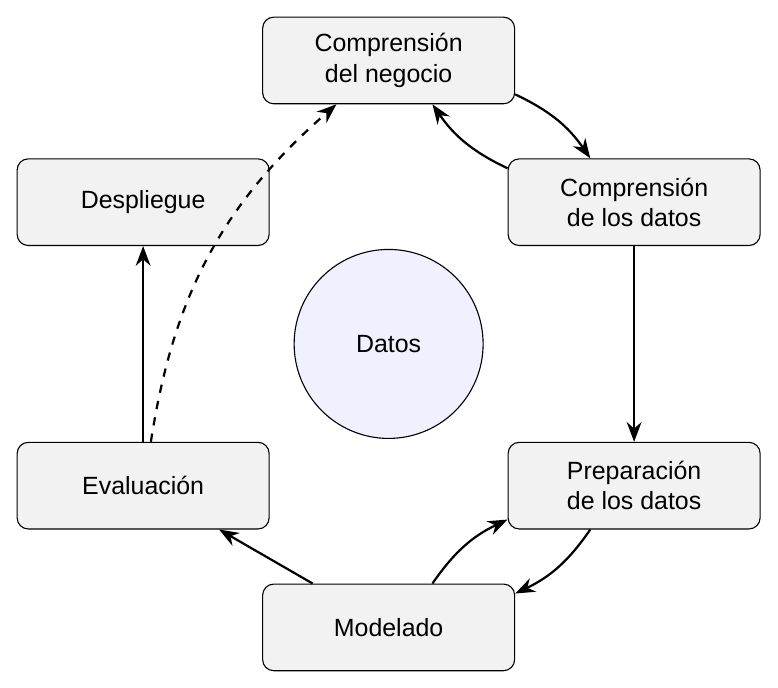
\includegraphics[width=0.6\textwidth]{imagenes/06_marco_teorico/crisp_dm.png}
  \fuente{Adaptado de \textcite{chapman2000}.}
\end{figure}

Una característica central de CRISP-DM es su carácter iterativo: la secuencia de fases no es
rígida, y el modelo contempla de forma explícita el retorno a fases anteriores cuando los
hallazgos lo requieren, por ejemplo cuando la exploración de los datos obliga a reformular
el objetivo o cuando el modelado revela la necesidad de nuevas variables. El ciclo externo
del diagrama de referencia (figura~\ref{fig:crisp-dm}) expresa, además, que el propio proceso
de minería de datos continúa tras el despliegue, porque las lecciones aprendidas generan
nuevas preguntas. La guía de referencia reconoce también que la preparación de los datos
suele concentrar la mayor parte del esfuerzo de un proyecto, un rasgo que se acentúa en
proyectos geoespaciales que integran fuentes heterogéneas.

CRISP-DM no es el único marco disponible. El proceso de descubrimiento de conocimiento en
bases de datos (KDD), descrito por \textcite{fayyad1996}, organiza el trabajo en etapas de
selección, preprocesamiento, transformación, minería de datos e interpretación o evaluación,
con un énfasis mayor en el proceso técnico de extracción de patrones que en la comprensión
del negocio. SEMMA, propuesto por SAS Institute, estructura el trabajo en las etapas de
muestreo, exploración, modificación, modelado y evaluación (\textit{Sample, Explore, Modify,
Model, Assess}), y está estrechamente asociado a las herramientas de ese proveedor. Frente a
ambos, CRISP-DM se distingue por incorporar explícitamente la comprensión del negocio y el
despliegue. En años recientes se han propuesto extensiones: \textcite{martinez2021}
analizaron la vigencia de CRISP-DM veinte años después de su creación y propusieron un marco
de trayectorias de ciencia de datos que reconoce que los proyectos actuales no siempre
siguen un ciclo lineal orientado a un modelo, sino recorridos exploratorios diversos; y
\textcite{studer2021} formularon CRISP-ML(Q), un modelo de proceso para aplicaciones de
aprendizaje automático con una metodología de aseguramiento de la calidad, que abarca seis
fases desde la definición del alcance hasta el mantenimiento de la aplicación desplegada,
ejecuta simultáneamente la comprensión del negocio y la de los datos, e incorpora de forma
explícita el monitoreo y el mantenimiento del modelo en operación frente a riesgos como la
deriva de los datos.

Se adopta CRISP-DM en este proyecto por su amplia aceptación en la práctica y en la
formación académica, por su énfasis en la comprensión del problema de la organización
destinataria y por su compatibilidad con las extensiones de CRISP-ML(Q) para la fase de
despliegue. Conforme a esta metodología, el proyecto se estructura de la siguiente manera.
En la comprensión del negocio se define el problema de los voluntarios de la Trufi
Association, que consiste en priorizar dónde revisar o mapear rutas, y se traduce en el
estimando del proyecto: el número esperado de consultas de cada zona dada su población y su
contexto territorial, cuyo contraste con lo observado orienta la priorización. En la
comprensión de los datos se exploran las consultas semanales y su distribución espacial y
temporal, se caracteriza el período sin datos de siete semanas, se examinan las ediciones de
población de Kontur y el feed GTFS de Trufi, y se analiza la autocorrelación espacial de las
consultas. En la preparación de los datos se depuran las consultas, se asignan a zonas H3 de
resolución~8, se integran con la población y con la cobertura medida como distancia al
trazado, y se construyen las macrozonas de resolución~6 que sirven como bloques de
validación. En el modelado se compara la escalera de técnicas descrita en
\ref{sec:tecnicas-algoritmos} mediante validación cruzada espacial por bloques. En la
evaluación se aplica una única vez el conjunto de prueba reservado, se calculan las métricas
descritas en \ref{sec:metricas}, se aplica la regla de selección declarada de antemano y se
realizan los análisis de sensibilidad y de estabilidad de la priorización. Finalmente, el
despliegue se limita a una propuesta de pipeline reproducible de actualización, que permita
reejecutar el proceso con nuevas consultas y nuevas ediciones de población y monitorear la
deriva de los datos al estilo de CRISP-ML(Q), junto con los entregables del proyecto, que
son un mapa interactivo, un archivo de estimaciones por zona y una lista de zonas
prioritarias para revisión, sin implementación operativa en los sistemas de Trufi.
    % 6. Marco Teórico
% ============================================================
%  7. DESARROLLO (SECCIÓN APLICATIVA: CRISP-DM)   (guía, 2.7 / Anexo A)
%  ------------------------------------------------------------
%  Aquí se documenta la EJECUCIÓN REAL del proyecto, organizada
%  según las seis fases de CRISP-DM.
%  Regla transversal de la guía: justificar decisiones, no
%  enumerar comandos ni librerías; interpretar resultados, no
%  solo mostrarlos.
%
%  Este archivo solo abre el capítulo e incluye las seis fases,
%  una por archivo, para poder trabajar sobre una sin tocar las
%  demás. Se incluyen con \input y no con \include porque las
%  fases son SECCIONES del mismo capítulo y no deben empezar en
%  página nueva.
% ============================================================
\chapter{Desarrollo (sección aplicativa: CRISP-DM)}
\label{cap:desarrollo}

% ============================================================
%  7.1. COMPRENSIÓN DEL NEGOCIO  -- parte del capítulo 7
%  ------------------------------------------------------------
%  Guía 2.7.1: (1) contexto operativo o institucional,
%  (2) traducción de la necesidad, (3) resultado esperado y
%  criterio de utilidad, (4) enlace con lo ya escrito.
%  No es "Comprensión de los datos" (fuentes, variables, EDA):
%  eso va en 08_02.
%  Fuente de verdad: trufi-data-science (EXPLICATIVO.md,
%  config.py, resultados/<fase>/metricas.json).
% ============================================================
\section{Comprensión del negocio}
\label{sec:comprension-negocio}

Esta primera fase de CRISP-DM define para quién se trabaja, qué decisión se quiere apoyar y
cómo se reconocerá que el resultado sirve. No trata todavía de los datos, que se describen
en la sección~\ref{sec:comprension-datos}, sino del proceso real de la organización y del
modo en que su necesidad se convierte en un problema que la Ciencia de Datos puede
abordar.

\subsection{Contexto operativo e institucional}
\label{sec:contexto-operativo}

Trufi Association es una organización sin fines de lucro que mantiene Trufi App, un
planificador de viajes para el transporte público del eje metropolitano de Cochabamba.
Como la mayor parte de ese transporte opera bajo la modalidad de paratránsito, sin
horarios ni paradas oficiales publicadas (sección~\ref{subsec:paratransito}), la
información que ofrece la aplicación no proviene de los operadores, sino de un
relevamiento colaborativo. El proceso real tiene cuatro pasos:
\begin{enumerate}
  \item Un grupo de voluntarios recorre una línea de micro o trufi.
  \item Los voluntarios registran su trayecto en OpenStreetMap
        (sección~\ref{subsec:cartografia-colaborativa}).
  \item El trazado se verifica con los operadores o en terreno.
  \item El trazado se convierte al formato GTFS (sección~\ref{subsec:gtfs}), que es el que
        consume el planificador de la aplicación.
\end{enumerate}
El feed resultante, empleado en este trabajo, describe 141 líneas de 43 operadores.

Cada jornada de mapeo consume desplazamientos, tiempo de edición y coordinación entre
personas que colaboran de forma voluntaria. Por eso la capacidad de la organización es
limitada, y cada jornada debe dirigirse a alguna zona concreta del territorio. Hoy esa
elección descansa en el conocimiento acumulado del equipo y en observaciones informales.
Al mismo tiempo, la aplicación genera de forma pasiva un registro de cada consulta de ruta
que realizan sus usuarios, con origen, destino, hora e identificador anónimo de
instalación. Ese registro abarca casi dos años (septiembre de 2022 a junio de 2024) y más
de 1,9~millones de consultas, pero no forma parte del proceso con el que se decide dónde
mapear. El punto de partida del proyecto es esa desconexión entre un proceso operativo que
necesita priorizar y un registro de uso que no se aprovecha para hacerlo.

\subsection{Traducción de la necesidad a un problema de Ciencia de Datos}
\label{sec:traduccion-necesidad}

La necesidad de la organización se expresa en términos operativos: \emph{¿a qué zonas
conviene enviar primero a los voluntarios?} Esa pregunta no puede responderse contando
consultas, porque un conteo bajo es ambiguo (sección~\ref{sec:descripcion-problema}).
Puede tratarse de una zona con poca población, o de una zona donde la aplicación no ofrece
información útil y, por eso, casi nadie la consulta. Para separar ambas situaciones hace
falta una referencia: cuántas consultas \emph{cabría esperar} en cada zona si se
comportara como las zonas comparables.

Con esa idea, la necesidad se traduce en un problema analítico de dos pasos:

\begin{enumerate}
  \item \textbf{Estimar el conteo esperado de consultas por zona.} Es un problema de
    regresión sobre datos de conteo (sección~\ref{subsec:datos-conteo}). La variable a
    estimar es el total de consultas originadas en cada zona H3 de resolución~8 durante el
    período, y la población residente actúa como \emph{exposición}: a igualdad de
    condiciones, una zona con el doble de habitantes debería generar el doble de consultas.
    Lo esperado se estima con información que no depende de la red mapeada: la población y
    la localización de la zona.
  \item \textbf{Comparar lo observado con lo esperado.} La diferencia entre ambos,
    expresada en una escala comparable entre zonas grandes y pequeñas, se denomina
    \emph{brecha} (sección~\ref{subsec:observado-esperado}). Una brecha negativa indica que
    la zona consulta menos de lo que cabría esperar por su población y su entorno. Esa
    señal, contrastada después con la cobertura de la red mapeada, orienta la revisión en
    terreno.
\end{enumerate}

Conviene precisar lo que el problema \emph{no} es. No es un pronóstico temporal, porque no
se predice cuántas consultas habrá la semana próxima, sino cuántas corresponden a cada zona
en el período observado. Tampoco es una clasificación de zonas en ``bien'' o ``mal''
mapeadas, porque no existe una etiqueta verificada de cobertura real con la cual entrenar
un clasificador. La cobertura de la red mapeada se excluye deliberadamente del cálculo de
lo esperado: si se incluyera, el modelo aprendería que las zonas sin rutas consultan poco y
les asignaría una expectativa baja, con lo que la brecha que se busca detectar desaparecería
por construcción.

\subsection{Resultado esperado y criterio de utilidad}
\label{sec:criterio-utilidad}

El resultado que se espera entregar a Trufi Association no es ``un modelo'', sino tres
productos que puedan usarse sin conocimientos de programación:
\begin{itemize}
  \item un archivo con el valor observado, el esperado y la brecha de cada zona;
  \item un mapa interactivo de la brecha;
  \item una lista corta de veinte zonas priorizadas para la revisión en terreno.
\end{itemize}
La mejora que se persigue es operativa: sustituir la elección informal entre más de mil
zonas por una lista corta, ordenada y justificada con datos.

Para que esa lista sea confiable, la técnica que produce el esperado debe cumplir criterios
medibles, fijados antes de ajustar cualquier modelo. La técnica se elegirá entre siete
alternativas de complejidad creciente. Sus códigos (B0 a B3 y M1 a M3) se explican en la
sección~\ref{sec:seleccion-algoritmos}. La tabla~\ref{tab:criterios-utilidad} resume los
criterios, cómo se mide cada uno y qué pregunta de la organización responde.

\begin{table}[H]
  \centering
  \caption{Criterios de utilidad declarados antes de modelar}
  \label{tab:criterios-utilidad}
  \interlineadoSimple
  \small
  \begin{tabularx}{\textwidth}{@{}L{0.23\textwidth}L{0.33\textwidth}Y@{}}
    \toprule
    \textbf{Criterio} & \textbf{Cómo se mide} & \textbf{Pregunta que responde} \\
    \midrule
    Supera al punto de referencia inicial & $D^2$ frente a la tasa global en zonas no vistas, mayor que cero & ¿El contexto territorial aporta algo más que la población? \\
    Ordena bien las zonas & Correlación de Spearman entre observado y esperado & ¿Las zonas que más consultan quedan arriba? \\
    Está calibrada & Suma de lo esperado dividida entre suma de lo observado, cercana a 1 & ¿El volumen total estimado es realista? \\
    Es estable & Índice de Jaccard del top-20 ante variaciones razonables & ¿La lista cambia si se modifica un supuesto menor? \\
    Es accionable & Número de zonas que el equipo debe revisar & ¿Se reduce el trabajo de decisión? \\
    \bottomrule
  \end{tabularx}
  \fuente{Elaboración propia. Las métricas se definen en la sección~\ref{sec:metricas}; los
  valores obtenidos se presentan en la sección~\ref{sec:evaluacion-resultados}.}
\end{table}

A estos criterios se suman dos reglas de protocolo, también declaradas de antemano. La
primera es que la técnica se elige con una regla escrita antes de ver los resultados, y no
por ser la primera que se probó ni la de menor error aparente
(sección~\ref{sec:regla-seleccion}). La segunda es que el conjunto de prueba se evalúa una
sola vez, al final.

La señal definitiva de utilidad, sin embargo, no es estadística. Sería la proporción de
zonas visitadas en las que los voluntarios encuentran rutas sin mapear. Esa verificación
en terreno excede el alcance de la materia (capítulo~\ref{cap:alcance}) y no se ha
realizado. Para que pueda medirse en cuanto empiecen las visitas, el archivo
\var{zonas_prioritarias.csv} incluye dos columnas de registro:
\begin{itemize}
  \item \var{field_result}, que registra el resultado de la visita con una de cuatro
        categorías: \var{ruta_no_mapeada}, \var{ruta_mapeada_correcta}, \var{sin_transporte}
        o \var{sin_visitar}. Esta última viene precargada en las veinte zonas.
  \item \var{field_notes}, que queda libre para observaciones.
\end{itemize}
El protocolo correspondiente se describe en la sección~\ref{sec:productos-despliegue}.

\subsection{Enlace con el problema, el alcance y los objetivos}
\label{sec:enlace-objetivos}

Esta fase concreta en términos operativos lo que los capítulos anteriores plantearon en
términos de investigación:
\begin{itemize}
  \item La ambigüedad del conteo descrita en el capítulo~\ref{cap:problema} se resuelve con
        la comparación entre lo observado y lo esperado.
  \item Las exclusiones del capítulo~\ref{cap:alcance} (sin pronóstico temporal, sin datos
        externos ni imputación de semanas faltantes, sin despliegue en producción) delimitan
        las técnicas admisibles y el tipo de entrega.
  \item Cada objetivo específico del capítulo~\ref{cap:objetivos} corresponde a una o dos
        fases de CRISP-DM y deja una evidencia verificable en el repositorio del proyecto,
        como se muestra en la tabla~\ref{tab:trazabilidad-oe}.
\end{itemize}

\begin{table}[H]
  \centering
  \caption{Correspondencia entre objetivos específicos, fases y evidencias}
  \label{tab:trazabilidad-oe}
  \interlineadoSimple
  \small
  \begin{tabularx}{\textwidth}{@{}L{0.07\textwidth}L{0.25\textwidth}L{0.17\textwidth}Y@{}}
    \toprule
    \textbf{OE} & \textbf{Fase y notebook} & \textbf{Sección} & \textbf{Evidencia principal} \\
    \midrule
    OE1 & Comprensión de los datos (\var{01_eda}); preparación (\var{02_preprocesamiento}, \var{03_feature_engineering}) & \ref{sec:comprension-datos} y \ref{sec:preparacion-datos} & Tabla de 1.628 zonas con consultas, población y cobertura; \var{metricas.json} de las tres fases \\
    OE2 & Preparación (reserva de prueba, \var{03_feature_engineering}); modelado (\var{04_modelado}) & \ref{sec:conjuntos-entrenamiento-prueba} y \ref{sec:modelado} & Bloques de prueba (\var{test_blocks.csv}); comparación de siete técnicas (\var{cv_resumen.csv}); regla de selección (\var{regla_seleccion.csv}) \\
    OE3 & Evaluación (\var{05_evaluacion}) & \ref{sec:evaluacion-resultados} & Métricas de prueba, brecha por zona, contraste con la cobertura y sensibilidad \\
    OE4 & Despliegue como propuesta (\var{06_propuesta}) & \ref{sec:despliegue} & Predicciones por zona, lista de veinte zonas prioritarias, mapa interactivo y procedimiento de actualización \\
    \bottomrule
  \end{tabularx}
  \fuente{Elaboración propia, a partir de la estructura del repositorio
  \var{trufi-data-science} (carpetas \var{notebooks/} y \var{resultados/}).}
\end{table}

La figura~\ref{fig:flujo-crisp-proyecto} muestra cómo se instanciaron las seis fases de
CRISP-DM en el proyecto. Cada fase de datos corresponde a un notebook que lee lo que dejó
la anterior, regenera sus salidas y termina con verificaciones automáticas de sus propias
cifras.

El carácter iterativo de la metodología (sección~\ref{sec:crisp-dm}) se manifestó en dos
retornos concretos a esta fase, señalados con flechas discontinuas en la figura:
\begin{itemize}
  \item El análisis exploratorio fijó la delimitación operativa del área de estudio, que
        el capítulo~\ref{cap:alcance} había dejado abierta a propósito
        (sección~\ref{sec:area-estudio}).
  \item La evaluación mostró que la lista de zonas con mayor brecha estaba formada casi por
        completo por zonas ya cubiertas por la red mapeada
        (sección~\ref{sec:interpretacion-resultados}). Como en esas zonas mapear no aporta,
        se precisó el criterio de utilidad: la lista priorizada se restringe a zonas sin
        trazado cercano.
\end{itemize}
La técnica elegida no se modificó por ese cambio. Ambas decisiones quedan documentadas
como tales, y no se presentan como parte del diseño original.

\begin{figure}[H]
  \centering
  \caption{Flujo CRISP-DM del proyecto: fases, notebooks y objetivos específicos}
  \label{fig:flujo-crisp-proyecto}
  \begin{tikzpicture}[
      font=\small,
      fase/.style={draw, rounded corners=3pt, fill=gray!8, align=center,
                   text width=4.0cm, minimum height=2.1cm, inner sep=3pt},
      flecha/.style={-{Stealth[length=2.5mm]}, thick},
      retorno/.style={-{Stealth[length=2.5mm]}, thick, dashed, gray!70!black},
      node distance=0.9cm and 0.45cm]
    \node[fase] (f1) {\textbf{1. Comprensión\\del negocio}\\[2pt] sección~\ref{sec:comprension-negocio}};
    \node[fase, right=of f1] (f2) {\textbf{2. Comprensión\\de los datos}\\[2pt] {\footnotesize\texttt{01\_eda}}\\ OE1};
    \node[fase, right=of f2, text width=5.0cm] (f3) {\textbf{3. Preparación\\de los datos}\\[2pt] {\footnotesize\texttt{02\_preprocesamiento}}\\ {\footnotesize\texttt{03\_feature\_engineering}}\\ OE1 y OE2};
    \node[fase, below=1.4cm of f3, text width=5.0cm] (f4) {\textbf{4. Modelado}\\[2pt] {\footnotesize\texttt{04\_modelado}}\\ OE2};
    \node[fase, left=of f4] (f5) {\textbf{5. Evaluación}\\[2pt] {\footnotesize\texttt{05\_evaluacion}}\\ OE3};
    \node[fase, left=of f5] (f6) {\textbf{6. Despliegue}\\ (propuesta)\\[2pt] {\footnotesize\texttt{06\_propuesta}}\\ OE4};
    \draw[flecha] (f1) -- (f2);
    \draw[flecha] (f2) -- (f3);
    \draw[flecha] (f3) -- (f4);
    \draw[flecha] (f4) -- (f5);
    \draw[flecha] (f5) -- (f6);
    \draw[retorno] (f2.north) to[bend right=25]
      node[above, font=\footnotesize, text=black] {delimitación del área} (f1.north);
    \draw[retorno] ($(f5.north west)+(0.5,0)$) --
      node[right, pos=0.5, font=\footnotesize, text=black] {regla de priorización}
      ($(f1.south east)+(-0.5,0)$);
  \end{tikzpicture}
  \fuente{Elaboración propia. Las flechas discontinuas señalan los dos retornos documentados
  a la comprensión del negocio.}
\end{figure}

% ============================================================
%  7.2. COMPRENSIÓN DE LOS DATOS  -- parte del capítulo 7
%  ------------------------------------------------------------
%  Guía 2.7.2: (1) fuentes, (2) variables y diccionario,
%  (3) EDA, (4) distribución, calidad, faltantes, atípicos y
%  relaciones, (5) gráficos y estadísticas, (6) hallazgos que
%  influyen en la preparación y el modelado.
%  Notebook: trufi-data-science/notebooks/01_eda.ipynb
%  Cifras:   resultados/01_eda/metricas.json y CSV de la carpeta.
% ============================================================
\section{Comprensión de los datos}
\label{sec:comprension-datos}

Esta fase examina las tres fuentes del proyecto antes de transformarlas. Tiene tres
propósitos:
\begin{itemize}
  \item medir su calidad;
  \item describir la variable que se va a estimar;
  \item fijar, con evidencia, los criterios que aplicará la preparación de los datos.
\end{itemize}
Se ejecuta en el notebook \var{01_eda}, que lee únicamente \var{data/raw/} y no escribe en
\var{data/}, de modo que ninguna decisión de limpieza se aplica todavía: solo se mide su
efecto. Las cifras de esta sección provienen de \var{resultados/01_eda/metricas.json} y de
los archivos CSV de la misma carpeta.

\subsection{Fuentes de datos}
\label{sec:fuentes-datos}

El proyecto emplea tres fuentes, todas conservadas sin modificar en \var{data/raw/}. La
tabla~\ref{tab:fuentes-datos} resume su origen, su contenido y las condiciones en que se
obtuvieron.

\begin{table}[H]
  \centering
  \caption{Fuentes de datos del proyecto}
  \label{tab:fuentes-datos}
  \interlineadoSimple
  \small
  \begin{tabularx}{\textwidth}{@{}L{0.20\textwidth}L{0.22\textwidth}Y@{}}
    \toprule
    \textbf{Fuente} & \textbf{Productor y obtención} & \textbf{Contenido y cobertura} \\
    \midrule
    Consultas de ``Trufi App'' & Trufi Association; exportaciones semanales del registro de la aplicación, entregadas para este trabajo & 85 archivos CSV que cubren 84 semanas ISO con datos, del 12-09-2022 al 09-06-2024 (la semana del 26-12-2022 al 01-01-2023 viene partida en dos archivos, sin filas repetidas); 1.927.675 consultas con origen, destino, fecha y hora, identificador anónimo de instalación, distancia y municipio de origen y destino \\
    Kontur Population, edición 2023-11-01 & Kontur; conjunto abierto descargado en formato GeoPackage comprimido & Población residente estimada por celda H3 de resolución~8 para toda Bolivia: 145.929 celdas y 12.431.735 habitantes (sección~\ref{subsec:kontur}) \\
    Feed GTFS de Trufi Cochabamba & Trufi Association; generado a partir del mapeo colaborativo en OpenStreetMap & 11 tablas: 43 operadores, 141 líneas y 626 recorridos con su trazado (una línea puede tener varios recorridos, por ejemplo ida y vuelta), 22.320 paradas y frecuencias; vigencia declarada desde el 01-01-2024 \\
    \bottomrule
  \end{tabularx}
  \fuente{Elaboración propia, a partir de \var{01_eda} (secciones 2 y 7) y
  \var{resultados/01_eda/metricas.json}.}
\end{table}

Las tres fuentes cumplen funciones distintas, y conviene fijarlas desde el inicio porque
condicionan todo lo que sigue:
\begin{itemize}
  \item Las \textbf{consultas} producen la variable objetivo, que es el número de consultas
        originadas en cada zona.
  \item \textbf{Kontur} aporta la exposición (la población residente) y las variables de
        entorno poblacional.
  \item El \textbf{GTFS} describe la red mapeada, y en este proyecto se usa solo para
        \emph{interpretar} la brecha, nunca como predictor (sección~\ref{sec:traduccion-necesidad}).
\end{itemize}
Una consulta es una búsqueda de ruta en la aplicación, no un viaje realizado: refleja la
necesidad de información de quienes usan ``Trufi App'', no la movilidad de toda la población
(sección~\ref{subsec:consultas-senal}).

\subsection{Variables y diccionario de datos}
\label{sec:diccionario-datos}

Las exportaciones de consultas llegaron en dos esquemas:
\begin{itemize}
  \item El \emph{lote original} reúne 79 archivos, desde 2022-W37 hasta 2024-W10. Tiene 13
        columnas en codificación UTF-8 y nombres temporales en español (\var{hora},
        \var{dia_de_semana}, \var{dia_de_mes}, \var{fin_de_semana}).
  \item El \emph{lote 2024} reúne 6 archivos, desde 2024-W18 hasta 2024-W23. Tiene 15
        columnas en codificación Latin-1, nombres temporales en inglés y dos campos nuevos
        (\var{year_week_number} y \var{time_of_day}).
\end{itemize}
La consolidación renombra los campos equivalentes a un nombre único y añade tres columnas
de linaje, que registran el archivo, el lote y la codificación de origen de cada fila. Con
ellas, cualquier registro puede rastrearse hasta su archivo. La
tabla~\ref{tab:diccionario-datos} describe las variables resultantes; las marcadas como
\emph{derivadas} no vienen en los archivos, sino que se calculan en la consolidación.

\begin{table}[H]
  \centering
  \caption{Diccionario de datos de las consultas consolidadas}
  \label{tab:diccionario-datos}
  \interlineadoSimple
  \small
  \begin{tabularx}{\textwidth}{@{}L{0.27\textwidth}L{0.13\textwidth}Y@{}}
    \toprule
    \textbf{Variable} & \textbf{Tipo} & \textbf{Significado} \\
    \midrule
    \var{date} & texto & Fecha y hora de la consulta (\texttt{AAAA-MM-DD hh:mm:ss}) \\
    \var{ts} & fecha-hora & Derivada: \var{date} convertida a marca de tiempo \\
    \var{year}, \var{week} & entero & Derivadas: año y semana ISO de \var{ts} \\
    \var{lat_orig}, \var{lon_orig} & real & Coordenadas del origen (WGS84); en el archivo, \var{origin_latitude} y \var{origin_longitude} \\
    \var{lat_dest}, \var{lon_dest} & real & Coordenadas del destino (WGS84) \\
    \var{userID} & texto & Identificador anónimo de la instalación de la aplicación (UUID); no identifica a una persona \\
    \var{distancia} & real & Distancia entre origen y destino; unidad verificada en la sección~\ref{sec:atipicos} (metros) \\
    \var{origin_municipio}, \var{dest_municipio} & texto & Municipio de origen y de destino asignado por la exportación \\
    \var{hour}, \var{day_of_week}, \var{day_of_month}, \var{weekend} & entero & Hora, día de la semana (0 = lunes), día del mes e indicador de fin de semana \\
    \var{year_week_number}, \var{time_of_day} & texto & Semana y franja del día; solo en el lote 2024 \\
    \var{source_file}, \var{source_batch}, \var{source_encoding} & texto & Derivadas: linaje (archivo, lote y codificación de origen) \\
    \bottomrule
  \end{tabularx}
  \fuente{Elaboración propia, a partir de los encabezados de \var{data/raw/*.csv},
  \var{src/lectura.py} y \var{resultados/01_eda/archivos_consultas.csv}.}
\end{table}

De Kontur se usan dos columnas: el identificador de la celda H3 (\var{h3_cell}) y su
población estimada (\var{population}), redondeada a entero. Del GTFS se usan los trazados
(\var{shapes.txt}), a partir de los cuales se calcula la distancia de cada zona a la red
mapeada, y las tablas de líneas, recorridos, paradas y frecuencias para describir la red.
Las variables que se construyen por zona a partir de estas fuentes se documentan en la
sección~\ref{sec:ingenieria-caracteristicas}.

\subsection{Análisis exploratorio de datos}
\label{sec:eda-recorrido}

El análisis exploratorio recorre las fuentes en el orden en que las usará la preparación.
Primero examina la calidad de las consultas, sus valores atípicos y su cobertura en el
tiempo. Después delimita el área de estudio y describe, dentro de ella, la red mapeada y
la población. Por último construye una versión \emph{candidata} de la variable objetivo:
el conteo de consultas por zona, obtenido aplicando en memoria los mismos filtros que
después ejecutará el preprocesamiento.

Trabajar con esa versión candidata tiene una ventaja: las relaciones y la dependencia
espacial se estudian sobre la misma unidad que se modelará, y no sobre consultas
individuales. Las funciones de limpieza que usa este notebook son las mismas que usa el
preprocesamiento (\var{src/limpieza.py}), de modo que las cifras de ambas fases coinciden
por construcción. El notebook termina con tres verificaciones automáticas:
\begin{itemize}
  \item el flujo de filtros cuadra con el total de consultas;
  \item el objetivo suma exactamente las consultas válidas;
  \item no quedan usuarios anómalos ni orígenes fuera del área.
\end{itemize}

\subsection{Calidad, datos faltantes y valores atípicos}
\label{sec:calidad-datos}

\subsubsection{Calidad y consistencia}

La calidad general de las consultas es alta. La tabla~\ref{tab:calidad-consultas} resume
los problemas detectados y su magnitud. En conjunto afectan a 3.097 de 1.927.675
consultas, es decir, al 0,16~\%.

\begin{table}[H]
  \centering
  \caption{Problemas de calidad detectados en las consultas}
  \label{tab:calidad-consultas}
  \interlineadoSimple
  \small
  \begin{tabularx}{\textwidth}{@{}L{0.30\textwidth}rY@{}}
    \toprule
    \textbf{Problema} & \textbf{Consultas} & \textbf{Interpretación} \\
    \midrule
    Origen en (0,0) & 3 & Coordenadas nulas registradas como cero; no localizables \\
    Origen fuera de Bolivia & 9 & Coordenadas imposibles para el servicio \\
    Copia exacta de otra consulta & 60 & Todas las columnas iguales (0,0031~\%); probable duplicación en la exportación \\
    Origen fuera del área de estudio & 2.509 & Consultas aisladas lejos del eje metropolitano (sección~\ref{sec:area-estudio}) \\
    Distancia mayor de 50~km & 283 & Pares origen--destino fuera de la escala urbana (sección~\ref{sec:atipicos}) \\
    Usuario anómalo & 233 & Consultas de dos instalaciones con uso no humano (sección~\ref{sec:atipicos}) \\
    \bottomrule
  \end{tabularx}
  \fuente{Elaboración propia, a partir de \var{resultados/01_eda/flujo_candidato.csv},
  \var{duplicados.csv} y \var{metricas.json}. Las cifras corresponden a la aplicación
  secuencial de los filtros; una consulta se cuenta en el primer filtro que la excluye.}
\end{table}

Los duplicados se examinaron con cuatro definiciones de creciente laxitud. Las copias
exactas y las que repiten origen, destino y marca de tiempo coinciden (60 en ambos casos).
Si se exige solo el mismo usuario y el mismo instante, aparecen 90. Como las 30 adicionales
difieren en el origen o el destino, pueden ser búsquedas legítimas distintas. Por eso solo
se considera duplicado lo que es idéntico en todas las columnas.

\subsubsection{Datos faltantes}
\label{sec:datos-faltantes-eda}

Ninguna de las columnas que usa el proyecto tiene valores nulos: coordenadas,
identificador, fecha y distancia están completas en ambos lotes. Las dos únicas columnas
con nulos, \var{year_week_number} y \var{time_of_day}, aparecen vacías en el 91,6~\% de
las filas. No es un faltante aleatorio, sino \emph{estructural}: esas columnas no existen en
el lote original. Como ambas pueden recalcularse a partir de la fecha, no se usan.

La ausencia de datos relevante para el proyecto está en otro nivel: faltan semanas enteras
de registro (sección~\ref{sec:cobertura-temporal}) y hay zonas pobladas sin ninguna
consulta (sección~\ref{sec:distribucion-objetivo}). Ninguna de las dos se imputa, en
coherencia con el alcance (capítulo~\ref{cap:alcance}) y con el tratamiento de datos
faltantes expuesto en la sección~\ref{subsec:datos-faltantes}. El hueco temporal se
documenta y se neutraliza al expresar lo esperado por semana observada. En cuanto a los
ceros, una zona poblada sin consultas es información, no ausencia de dato.

\subsubsection{Valores atípicos: distancia y usuarios anómalos}
\label{sec:atipicos}

\textbf{Distancia.} El campo \var{distancia} no traía unidad declarada. Para verificarla,
se comparó con la distancia geodésica entre origen y destino calculada de forma
independiente, en una muestra de 200.000 consultas. El error relativo mediano fue del
0,142~\%, lo que confirma que el campo está en metros y corresponde a la distancia en
línea recta.

La distribución (figura~\ref{fig:distancia}) muestra el comportamiento esperado de un
servicio urbano:
\begin{itemize}
  \item la mediana es de 3,39~km;
  \item el 90~\% de las consultas no supera los 10,26~km;
  \item el percentil 99,9 llega a 40,7~km.
\end{itemize}
Por encima de 50~km aparece una cola dispersa (el 0,04~\% de las consultas) que llega a
miles de kilómetros y que no corresponde a viajes posibles en la red urbana.

\begin{figure}[H]
  \centering
  \caption{Distribución de la distancia origen--destino de las consultas}
  \label{fig:distancia}
  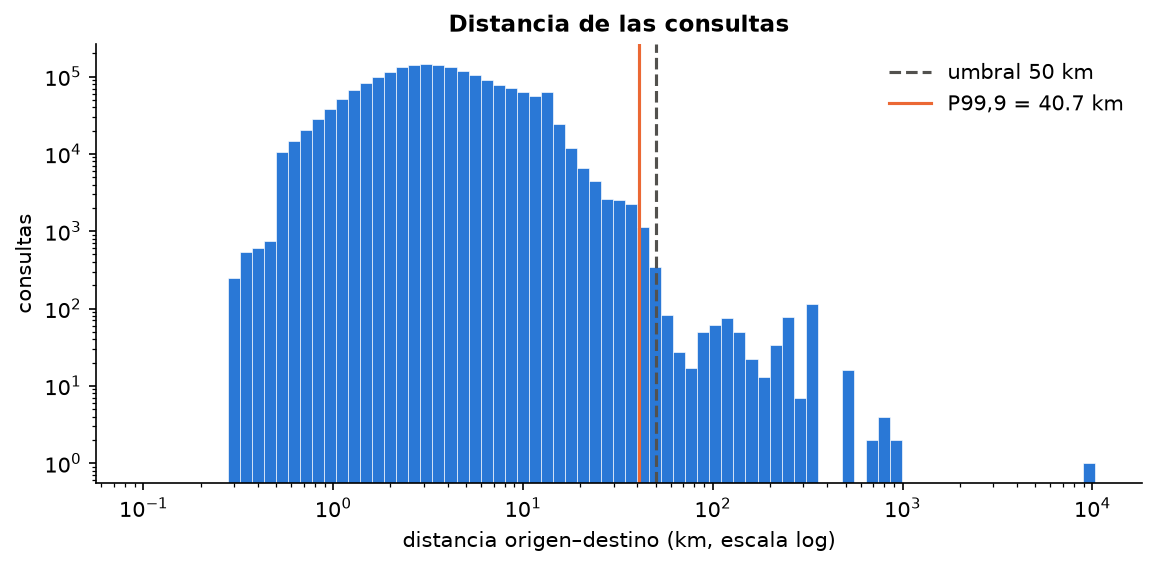
\includegraphics[width=0.75\textwidth]{imagenes/07_desarrollo/7_2_comprension_datos/distancia.png}
  \fuente{Elaboración propia, a partir de \var{01_eda} (sección 3). Ambos ejes en escala
  logarítmica; la línea discontinua marca el umbral de 50~km.}
\end{figure}

El umbral de 50~km se aplica a las \emph{consultas} y no a la delimitación del área. Una
consulta con destino lejano puede tener un origen perfectamente válido dentro de la
ciudad. Si el área se recortara con ese criterio, zonas reales quedarían fuera.

\textbf{Usuarios anómalos.} Hay 130.545 identificadores de instalación distintos. Para
detectar un uso no humano, por ejemplo pruebas automatizadas o extracción masiva de
rutas, se definieron seis señales por usuario, con umbrales fijados en \var{config.py}:
\begin{itemize}
  \item más de 1.000 consultas en total (volumen);
  \item más de 50 consultas por día activo (intensidad);
  \item más de 200 zonas de origen distintas (dispersión);
  \item más de 100 consultas en un mismo día (ráfaga);
  \item menos del 5~\% de pares origen--destino repetidos entre usuarios con más de 100
        consultas (sin rutina);
  \item un intervalo mediano menor de 60~segundos entre consultas consecutivas (rapidez).
\end{itemize}

La tabla~\ref{tab:senales-usuario} muestra cuántos usuarios activan cada señal y justifica
que se exijan al menos dos. La señal de rapidez, por sí sola, marcaría a 10.511
instalaciones. Esas instalaciones corresponden a un comportamiento humano habitual:
repetir una búsqueda o corregir el destino en pocos segundos. Exigir dos señales
simultáneas deja solo dos instalaciones anómalas, con 233 consultas en total.

\begin{table}[H]
  \centering
  \caption{Usuarios que activan cada señal de uso anómalo}
  \label{tab:senales-usuario}
  \interlineadoSimple
  \small
  \begin{tabular}{@{}lr@{}}
    \toprule
    \textbf{Señal} & \textbf{Usuarios} \\
    \midrule
    Volumen ($>$ 1.000 consultas) & 1 \\
    Intensidad ($>$ 50 consultas por día activo) & 1 \\
    Dispersión ($>$ 200 zonas de origen) & 0 \\
    Ráfaga ($>$ 100 consultas en un día) & 1 \\
    Sin rutina ($<$ 5~\% de pares repetidos) & 0 \\
    Rapidez (intervalo mediano $<$ 60~s) & 10.511 \\
    \midrule
    \textbf{Marcados como anómalos ($\geq$ 2 señales)} & \textbf{2} \\
    \bottomrule
  \end{tabular}
  \fuente{Elaboración propia, a partir de \var{resultados/01_eda/usuarios_senales.csv} y
  \var{src/limpieza.py}.}
\end{table}

\subsection{Distribución temporal y espacial}
\label{sec:distribucion-datos}

\subsubsection{Cobertura temporal}
\label{sec:cobertura-temporal}

El período declarado va del 12 de septiembre de 2022 al 9 de junio de 2024, es decir,
91 semanas ISO. Hay datos en 84 de ellas, repartidos en 85 archivos: la semana que va del
26 de diciembre de 2022 al 1 de enero de 2023 se exportó en dos archivos, uno con los días
26 a 31 de diciembre (11.622 consultas) y otro con el 1 de enero (695), sin filas repetidas
entre ambos. De las 84 semanas, 78 tienen registros los siete días. Faltan
siete semanas consecutivas, del 11 de marzo al 28 de abril de 2024, sin ninguna consulta
(figura~\ref{fig:cobertura-semanal}).

\begin{figure}[H]
  \centering
  \caption{Consultas por semana y hueco sin datos de 2024}
  \label{fig:cobertura-semanal}
  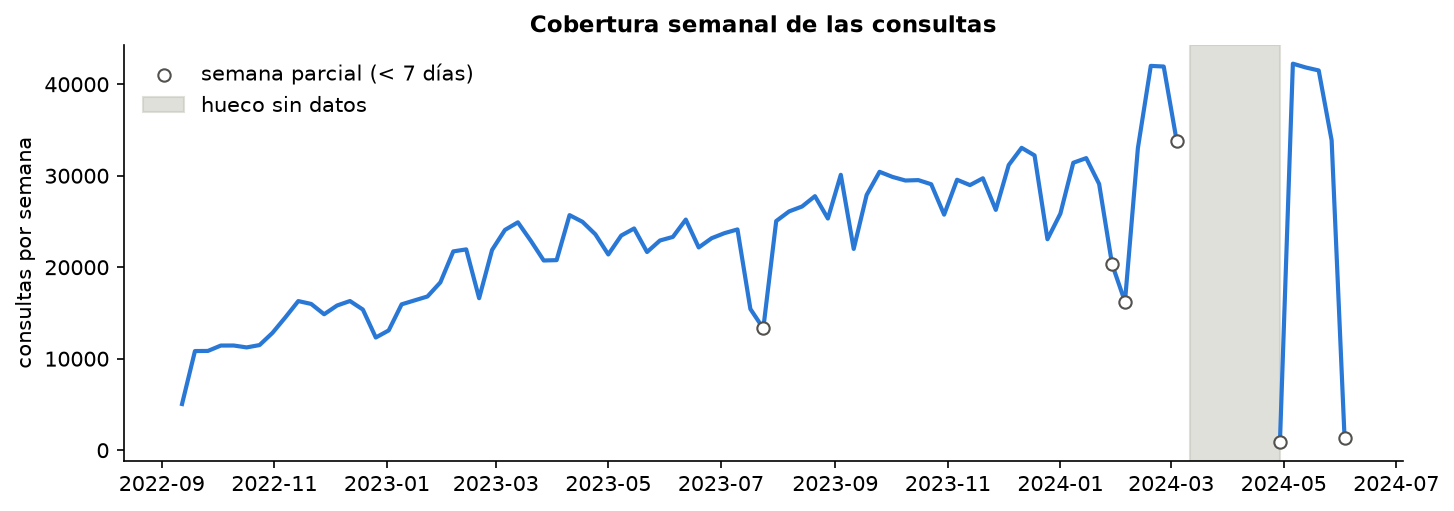
\includegraphics[width=\textwidth]{imagenes/07_desarrollo/7_2_comprension_datos/cobertura_semanal.png}
  \fuente{Elaboración propia, a partir de \var{01_eda} (sección 5). Los círculos marcan
  semanas parciales (menos de siete días con datos).}
\end{figure}

La serie muestra un crecimiento sostenido del uso: de unas 11.000 consultas semanales a
fines de 2022 a más de 30.000 a fines de 2023. La media semanal pasa de 22.731 consultas
antes del hueco a 39.864 después. El hueco coincide exactamente con el cambio de esquema:
el lote 2024, con dos columnas nuevas y otra codificación, empieza en la primera semana
posterior. Esa coincidencia sugiere una interrupción del proceso de exportación, y no una
caída real del uso.

El conjunto de datos disponible corresponde a las exportaciones que Trufi Association pudo
extraer y entregar en el plazo del proyecto; el resto del registro continúa en proceso de
exportación. El hueco de siete semanas y el cambio de esquema son consistentes con esa
interrupción, aunque la causa exacta no pudo confirmarse. Esta limitación se retoma en la
sección~\ref{sec:limitaciones} y en la recomendación R8. El registro es, por tanto,
parcial y puede ampliarse, y los resultados describen los datos entregados.

El hueco no afecta a la unidad de análisis, que es el total de consultas por zona
acumulado en todo el período. Sí afecta a la lectura de ese total como volumen semanal.
Por eso la preparación calcula las semanas equivalentes realmente observadas
(sección~\ref{sec:transformaciones}), y la evaluación comprueba si la lista de zonas
cambia al usar solo el período anterior al hueco (sección~\ref{sec:interpretacion-resultados}).

El perfil horario y semanal (figura~\ref{fig:perfil-temporal}) confirma que el registro
refleja un uso cotidiano de transporte:
\begin{itemize}
  \item la actividad crece desde las 6~h y alcanza su máximo a las 14~h, con el 8,2~\% de
        las consultas;
  \item los días laborables reúnen entre el 14~\% y el 17~\% de las consultas cada uno;
  \item el fin de semana concentra el 22,8~\%, y el domingo es el día de menor uso.
\end{itemize}
Este perfil no se modela, porque el alcance excluye la dimensión temporal. Se incluye como
evidencia de que las consultas corresponden a necesidades reales de desplazamiento y no a
tráfico artificial.

\begin{figure}[H]
  \centering
  \caption{Distribución de las consultas por hora del día y por día de la semana}
  \label{fig:perfil-temporal}
  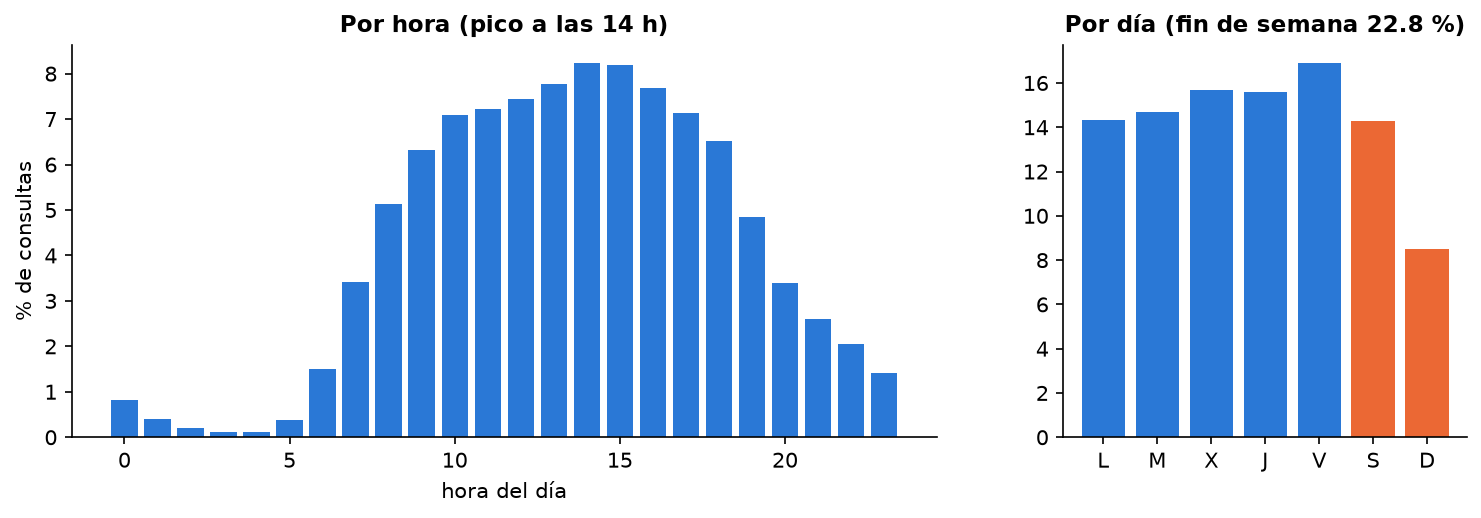
\includegraphics[width=\textwidth]{imagenes/07_desarrollo/7_2_comprension_datos/perfil_temporal.png}
  \fuente{Elaboración propia, a partir de \var{01_eda} (sección 5) y
  \var{resultados/01_eda/perfil_temporal.csv}.}
\end{figure}

\subsubsection{Distribución espacial y área de estudio}
\label{sec:area-estudio}

El alcance dejó abierta la delimitación operativa del entorno del eje metropolitano
(capítulo~\ref{cap:alcance}), y esta fase la fija a partir de los propios datos. El primer
intento fue la envolvente de todas las zonas H3 con al menos un origen válido, que
abarcaría 485.940,1~km\textsuperscript{2}, más de un tercio de la superficie de Bolivia.
El motivo es que unas pocas consultas aisladas, muy alejadas, estiran el contorno. Ese
resultado muestra que un área definida por los datos crudos es frágil ante atípicos
geográficos.

La solución adoptada identifica la \emph{componente contigua principal} de las zonas H3
con orígenes válidos. Esa componente es el mayor conjunto de zonas conectadas entre sí por
vecindad directa. El área es su envolvente, ampliada con un margen de 1~km. La
tabla~\ref{tab:variantes-area} compara esta opción con otras más laxas, en las que dos
zonas se consideran conectadas aunque estén separadas por uno o dos anillos vacíos.

\begin{table}[H]
  \centering
  \caption{Variantes de delimitación del área de estudio}
  \label{tab:variantes-area}
  \interlineadoSimple
  \small
  \begin{tabular}{@{}lrr@{}}
    \toprule
    \textbf{Variante} & \textbf{Zonas H3} & \textbf{Área (km\textsuperscript{2})} \\
    \midrule
    Todas las zonas con orígenes válidos & 1.516 & 485.940,1 \\
    \textbf{Componente contigua, vecindad directa ($k=1$)} & \textbf{919} & \textbf{1.505,7} \\
    Componente con separación de hasta un anillo ($k=2$) & 1.076 & 1.965,4 \\
    Componente con separación de hasta dos anillos ($k=3$) & 1.195 & 3.040,9 \\
    \bottomrule
  \end{tabular}
  \fuente{Elaboración propia, a partir de \var{resultados/01_eda/area_variantes.csv}. El área
  incluye el margen de 1~km.}
\end{table}

La variante elegida mide 1.505,7~km\textsuperscript{2} y contiene el 99,87~\% de los
orígenes válidos (figura~\ref{fig:area-estudio}). Las variantes más laxas duplican el área
para ganar una fracción mínima de consultas, a costa de incorporar zonas rurales casi sin
uso. Las 2.509 consultas que quedan fuera son las que la
tabla~\ref{tab:calidad-consultas} registra como ``origen fuera del área de estudio''.

\begin{figure}[H]
  \centering
  \caption{Orígenes de las consultas y área de estudio delimitada}
  \label{fig:area-estudio}
  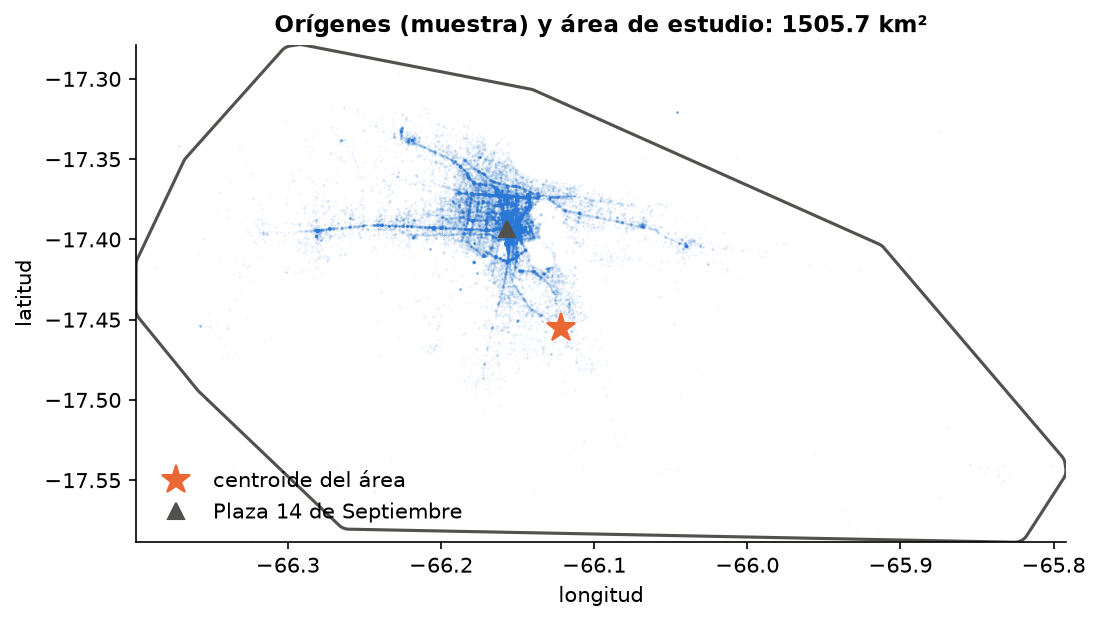
\includegraphics[width=0.85\textwidth]{imagenes/07_desarrollo/7_2_comprension_datos/area_estudio.png}
  \fuente{Elaboración propia, a partir de \var{01_eda} (sección 6). Puntos: muestra de
  orígenes; contorno: área de estudio; triángulo: Plaza 14 de Septiembre; estrella:
  centroide geométrico del área.}
\end{figure}

La figura revela además un hecho que se retoma en la preparación: el centroide geométrico
del área está a 7,82~km de la Plaza 14 de Septiembre, fuera del núcleo donde se concentran
los orígenes. Un ``centro'' calculado a partir de la forma del área no representa el
centro de actividad de la ciudad.

Dentro del área se localizan 1.577 celdas de Kontur (por la posición de su centroide), con
1.223.871 habitantes. De ellas, 609 no registran ningún origen de consulta en los datos
sin depurar; tras la limpieza son 611, porque dos celdas solo tenían consultas que la limpieza
excluyó (sección~\ref{sec:limpieza}). Además, 202 tienen
menos de 10 habitantes. La red mapeada cubre la mayor parte del territorio con demanda
(figura~\ref{fig:gtfs-red}): el 99,47~\% de los orígenes está a 500~m o menos de algún
trazado GTFS. Los trazados tienen una longitud mediana de 20,22~km y suman
12.737,3~km. La frecuencia mediana declarada es de un servicio cada 5~minutos.

\begin{figure}[H]
  \centering
  \caption{Trazados de la red mapeada (GTFS) y orígenes de las consultas}
  \label{fig:gtfs-red}
  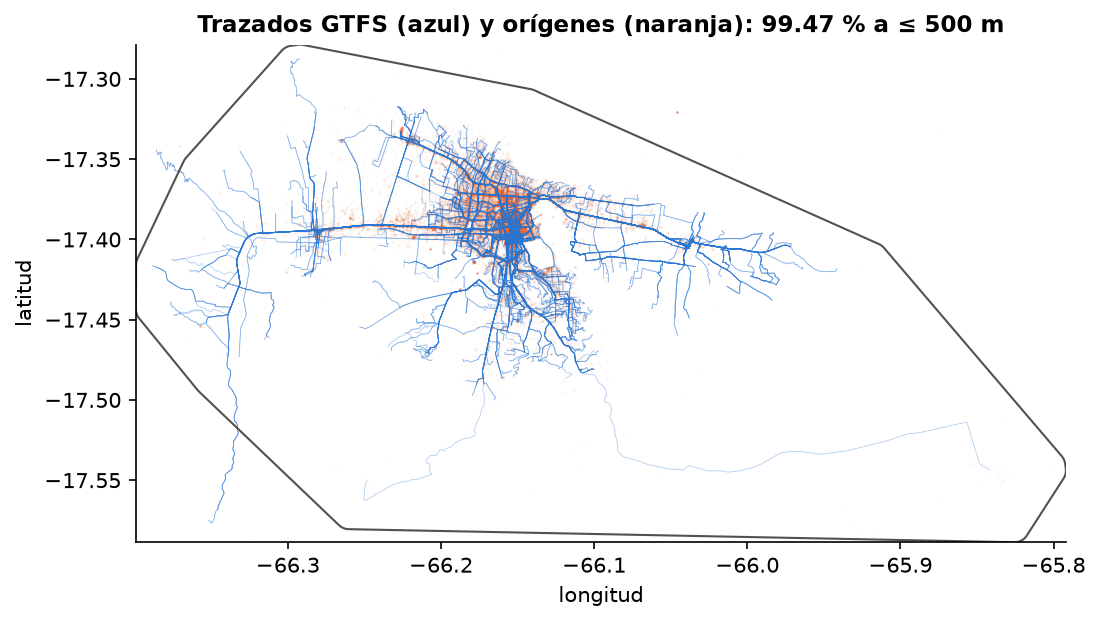
\includegraphics[width=0.85\textwidth]{imagenes/07_desarrollo/7_2_comprension_datos/gtfs_red_y_demanda.png}
  \fuente{Elaboración propia, a partir de \var{01_eda} (sección 7). Azul: trazados de
  \var{shapes.txt}; naranja: orígenes.}
\end{figure}

Que casi todos los orígenes estén cerca de un trazado no implica que la red esté completa.
Las consultas nacen donde la aplicación ya es útil: una zona sin rutas mapeadas genera
pocas consultas precisamente porque la aplicación no le ofrece respuestas. Este sesgo de
selección es la razón por la que la cobertura no puede usarse para estimar lo esperado
(sección~\ref{sec:traduccion-necesidad}). También hay que tener en cuenta que el feed
declara una vigencia posterior a buena parte del período de consultas, una limitación ya
reconocida en el capítulo~\ref{cap:alcance}.

\subsubsection{Distribución de la variable objetivo}
\label{sec:distribucion-objetivo}

La variable objetivo candidata, \var{query_count}, es el número de consultas válidas
originadas en cada zona H3 de resolución~8 durante el período. Dentro del área hay 1.628
zonas. Para que una tasa por habitante sea estable, se exige un mínimo de 10 habitantes;
1.381 zonas lo cumplen. La figura~\ref{fig:objetivo-distribucion} resume la distribución
del conteo en esas 1.381 zonas.

\begin{figure}[H]
  \centering
  \caption{Distribución del conteo de consultas por zona y curva de Lorenz}
  \label{fig:objetivo-distribucion}
  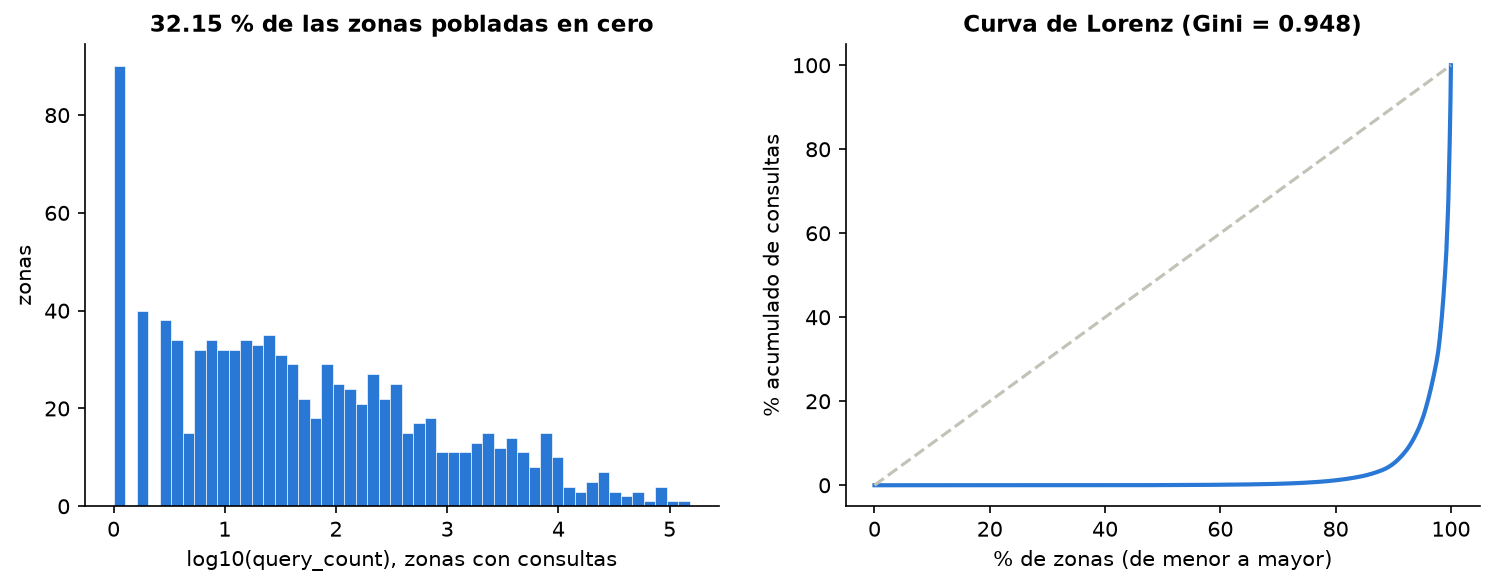
\includegraphics[width=\textwidth]{imagenes/07_desarrollo/7_2_comprension_datos/objetivo_distribucion.png}
  \fuente{Elaboración propia, a partir de \var{01_eda} (sección 9). Izquierda: histograma de
  $\log_{10}$ del conteo en las zonas con consultas; derecha: proporción acumulada de
  consultas frente a proporción acumulada de zonas.}
\end{figure}

Tres rasgos caracterizan la distribución y condicionan el modelado:
\begin{itemize}
  \item \textbf{Abundancia de ceros.} El 32,15~\% de las zonas pobladas (444 de 1.381) no
        registra ninguna consulta. Esos ceros se conservan: son justamente el tipo de zona
        que el problema busca examinar (capítulo~\ref{cap:problema}).
  \item \textbf{Concentración extrema.} El coeficiente de Gini es de 0,948, y las diez
        zonas con más consultas reúnen el 42~\% del total. Como muestra la curva de Lorenz,
        el 80~\% de las zonas aporta menos del 5~\% de las consultas.
  \item \textbf{Sobredispersión.} La varianza del conteo es 46.569 veces su media. Un modelo
        de Poisson supone varianza igual a la media
        (sección~\ref{subsec:datos-conteo}), así que este resultado anticipa que ese
        supuesto no se cumplirá y justifica incluir alternativas que lo relajen.
\end{itemize}

\subsection{Relaciones entre variables y dependencia espacial}
\label{sec:relaciones-variables}

Para examinar qué información territorial se asocia con las consultas, se calculó la
correlación de Spearman entre el conteo por zona y cada variable candidata. La correlación
de Spearman se basa en rangos, por lo que es robusta a la asimetría de los datos. Se
calculó también frente a la \emph{tasa} de consultas por 1.000 habitantes, para distinguir
la asociación que se debe solo al tamaño de la población de la que se debe al contexto. La
tabla~\ref{tab:relaciones} presenta los resultados.

\begin{table}[H]
  \centering
  \caption{Correlación de Spearman de las variables candidatas con el conteo y con la tasa}
  \label{tab:relaciones}
  \interlineadoSimple
  \small
  \begin{tabularx}{\textwidth}{@{}L{0.22\textwidth}Yrr@{}}
    \toprule
    \textbf{Variable} & \textbf{Significado} & \textbf{Conteo} & \textbf{Tasa} \\
    \midrule
    \var{population} & Habitantes de la zona (Kontur) & 0,855 & 0,710 \\
    \var{pop_ring1} & Habitantes del primer anillo de seis zonas vecinas & 0,836 & 0,721 \\
    \var{pop_ring2} & Habitantes del segundo anillo de vecinas & 0,804 & 0,701 \\
    \var{dist_centro_km} & Distancia a la Plaza 14 de Septiembre (km) & $-0{,}697$ & $-0{,}677$ \\
    \var{dist_centroide_km} & Distancia al centroide geométrico del área (km) & $-0{,}476$ & $-0{,}485$ \\
    \var{dist_trazado_m} & Distancia al trazado GTFS más cercano (m); solo contraste & $-0{,}763$ & $-0{,}701$ \\
    \bottomrule
  \end{tabularx}
  \fuente{Elaboración propia, a partir de \var{resultados/01_eda/relaciones.csv}; 1.381 zonas
  con al menos 10 habitantes.}
\end{table}

De la tabla se desprenden tres lecturas:
\begin{itemize}
  \item La población es la variable más asociada con el conteo, lo que justifica tratarla
        como exposición. Las variables de entorno siguen asociadas con la \emph{tasa}
        (0,72 para la población vecina y $-0{,}68$ para la distancia al centro), de modo que
        el contexto aporta información más allá del tamaño de la zona.
  \item La distancia a la Plaza se asocia bastante más que la distancia al centroide del
        área ($-0{,}697$ frente a $-0{,}476$), lo que confirma que el centro de referencia
        debe fijarse de forma externa a los datos y no derivarse de la forma del área.
  \item La distancia al trazado GTFS tiene una asociación fuerte, pero se reserva para el
        contraste por el sesgo de selección descrito en la sección~\ref{sec:area-estudio}.
\end{itemize}

La figura~\ref{fig:objetivo-poblacion} muestra la relación con la población en escala
logarítmica. La asociación es clara, pero la dispersión es enorme: zonas con población
similar difieren en varios órdenes de magnitud. Las zonas alejadas del trazado (en
naranja) se concentran en la parte baja.

\begin{figure}[H]
  \centering
  \caption{Consultas por zona frente a su población, según la distancia al trazado}
  \label{fig:objetivo-poblacion}
  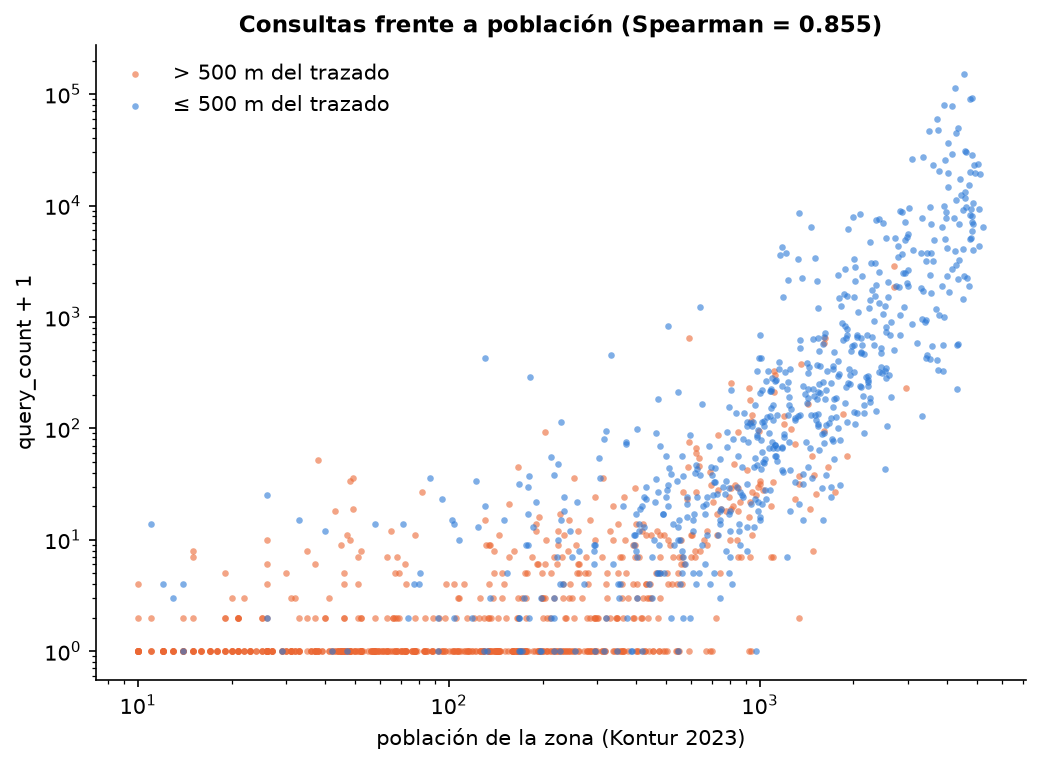
\includegraphics[width=0.75\textwidth]{imagenes/07_desarrollo/7_2_comprension_datos/objetivo_vs_poblacion.png}
  \fuente{Elaboración propia, a partir de \var{01_eda} (sección 10). Ambos ejes en escala
  logarítmica; al conteo se le suma 1 para representar los ceros.}
\end{figure}

\textbf{Dependencia espacial.} Se midió con el índice $I$ de Moran de la tasa de consultas
(sección~\ref{subsec:autocorrelacion}), tomando como vecinas las zonas situadas a $k$
anillos H3 de distancia, con $k$ de 1 a 5. La significación se evaluó con 499
permutaciones, por lo que el menor $p$-valor alcanzable es 0,002.

\begin{table}[H]
  \centering
  \caption{Correlograma del índice de Moran de la tasa de consultas}
  \label{tab:correlograma}
  \interlineadoSimple
  \small
  \begin{tabular}{@{}crrr@{}}
    \toprule
    \textbf{\celda{Orden de\\vecindad $k$}} & \textbf{\celda{Distancia\\aproximada (km)}} & \textbf{$I$ de Moran} & \textbf{$p$-valor} \\
    \midrule
    1 & 0,92 & 0,7161 & 0,002 \\
    2 & 1,84 & 0,6399 & 0,002 \\
    3 & 2,76 & 0,5773 & 0,002 \\
    4 & 3,68 & 0,5094 & 0,002 \\
    5 & 4,60 & 0,4603 & 0,002 \\
    \bottomrule
  \end{tabular}
  \fuente{Elaboración propia, a partir de \var{resultados/01_eda/autocorrelacion.csv}.}
\end{table}

El correlograma (tabla~\ref{tab:correlograma}) muestra una autocorrelación positiva muy
fuerte entre vecinas inmediatas ($I = 0{,}72$), que decae lentamente y sigue en 0,46 a
unos 4,6~km. El indicador local LISA (figura~\ref{fig:lisa}) localiza esa estructura:
\begin{itemize}
  \item un gran núcleo de 295 zonas \emph{alto-alto} (tasa alta rodeada de tasas altas) en
        el centro y los ejes de Cercado y Sacaba;
  \item 253 zonas \emph{bajo-bajo} en la periferia y en el sur del valle;
  \item pocos casos discordantes (41 alto-bajo y 3 bajo-alto).
\end{itemize}

\begin{figure}[H]
  \centering
  \caption{Agrupamientos locales de la tasa de consultas (LISA)}
  \label{fig:lisa}
  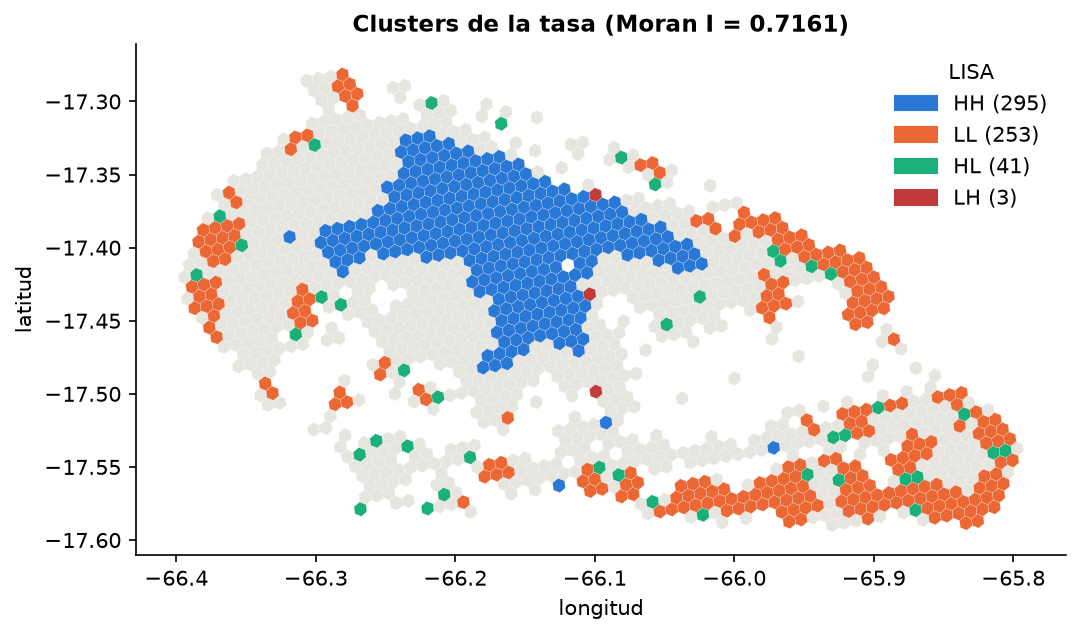
\includegraphics[width=0.85\textwidth]{imagenes/07_desarrollo/7_2_comprension_datos/lisa.png}
  \fuente{Elaboración propia, a partir de \var{01_eda} (sección 11). HH: alto-alto;
  LL: bajo-bajo; HL: alto-bajo; LH: bajo-alto; gris: sin agrupamiento significativo.}
\end{figure}

Este hallazgo tiene dos consecuencias metodológicas directas:
\begin{itemize}
  \item Las zonas vecinas se parecen, de modo que una partición aleatoria en entrenamiento
        y prueba colocaría a cada zona de prueba junto a vecinas casi idénticas y
        sobreestimaría el desempeño. La validación y la reserva de prueba deben hacerse por
        \emph{bloques} espaciales de varios kilómetros (sección~\ref{subsec:validacion-espacial}).
  \item La tasa de las zonas vecinas contiene información útil para estimar la de una zona,
        lo que motiva incluir entre las técnicas un estimador de vecindad
        (sección~\ref{sec:seleccion-algoritmos}).
\end{itemize}

\subsection{Estadísticas descriptivas del conjunto de datos H3}
\label{sec:estadisticas-descriptivas}

La tabla~\ref{tab:descriptivos} reúne las estadísticas de las variables numéricas por zona
que se usan en las fases siguientes. Se calculan sobre las 1.381 zonas que entrarán al
modelo.

\begin{table}[H]
  \centering
  \caption{Estadísticas descriptivas de las variables por zona}
  \label{tab:descriptivos}
  \interlineadoSimple
  \small
  \begin{tabular}{@{}lrrrrrrr@{}}
    \toprule
    \textbf{Variable} & \textbf{Media} & \textbf{Desv. est.} & \textbf{Mín.} & \textbf{P25} & \textbf{Mediana} & \textbf{P75} & \textbf{Máx.} \\
    \midrule
    \var{query_count} (consultas) & 1.393,4 & 8.058,4 & 0 & 0 & 6 & 109 & 152.494 \\
    \var{population} (hab.) & 887,5 & 1.162,6 & 10 & 97 & 388 & 1.183 & 5.240 \\
    \var{pop_ring1} (hab.) & 5.221,8 & 6.363,6 & 3 & 799 & 2.398 & 7.613 & 28.988 \\
    \var{dist_centro_km} (km) & 17,0 & 9,4 & 0,5 & 9,7 & 15,9 & 22,1 & 41,8 \\
    \bottomrule
  \end{tabular}
  \fuente{Elaboración propia, a partir de
  \var{resultados/03_feature_engineering/estadisticas_descriptivas.csv}; 1.381 zonas con al
  menos 10 habitantes.}
\end{table}

La distancia entre la media (1.393 consultas) y la mediana (6) del conteo resume la
asimetría: la zona típica tiene muy pocas consultas, y un puñado de zonas centrales
concentra casi todo el volumen. El percentil 25 del conteo es 0, reflejo del 32~\% de
zonas pobladas sin consultas. En cuanto a la cobertura, algo más de la mitad de las zonas
del modelo no tiene un trazado a 500~m o menos: son 755 zonas (el 54,7~\%), pero reúnen
solo 200.041 habitantes, el 16~\% de la población del modelo
(\var{resultados/05_evaluacion/contraste_gtfs.csv}).

Las tablas~\ref{tab:descriptivos}, \ref{tab:municipios} y~\ref{tab:anillos} se calculan en
\var{03_feature_engineering} y se guardan en
\var{resultados/03_feature_engineering/estadisticas_descriptivas.csv},
\var{resumen_municipio.csv} y \var{resumen_anillo.csv}, respectivamente.

\subsection{Registro de hallazgos y decisiones}
\label{sec:hallazgos-decisiones}

La tabla~\ref{tab:trazabilidad-hallazgos} reúne los hallazgos de esta fase que modifican
alguna decisión posterior. Cada uno se vincula con la fase en la que actúa. Los hallazgos
descriptivos que no cambian ninguna decisión, como el perfil horario, no se incluyen.

\begin{table}[H]
  \centering
  \caption{Hallazgos de la comprensión de los datos y decisiones que habilitan}
  \label{tab:trazabilidad-hallazgos}
  \interlineadoSimple
  \small
  \begin{tabularx}{\textwidth}{@{}L{0.30\textwidth}YL{0.16\textwidth}@{}}
    \toprule
    \textbf{Hallazgo} & \textbf{Decisión} & \textbf{Fase} \\
    \midrule
    La envolvente de todos los orígenes abarca 485.940~km\textsuperscript{2} & Área = componente H3 contigua más 1~km (1.505,7~km\textsuperscript{2}) & Preparación \\
    Cola de distancias mayores de 50~km (0,04~\%) & Excluir esas consultas, sin recortar el área & Preparación \\
    Una sola señal marca a 10.511 usuarios legítimos & Usuario anómalo = al menos 2 de 6 señales (2 usuarios) & Preparación \\
    60 copias exactas & Conservar la primera aparición & Preparación \\
    Hueco de 7 semanas en 2024 & No imputar; expresar lo esperado por semana observada; sensibilidad sin el período posterior & Preparación y evaluación \\
    32,15~\% de zonas pobladas sin consultas & Conservar los ceros; no imputar & Preparación y modelado \\
    El centroide del área no representa el centro de actividad & Centro de referencia exógeno: Plaza 14 de Septiembre & Preparación \\
    Autocorrelación espacial persistente hasta unos 4,6~km & Validación y prueba por bloques H3 de resolución~6 (unos 36~km\textsuperscript{2}); estimador de vecindad entre las técnicas & Preparación y modelado \\
    Varianza 46.569 veces la media & Modelos de conteo con la población como exposición; incluir la binomial negativa & Modelado \\
    Orígenes concentrados cerca de la red mapeada & GTFS solo para contraste, nunca como predictor & Preparación y evaluación \\
    \bottomrule
  \end{tabularx}
  \fuente{Elaboración propia, a partir de \var{01_eda} (sección 13, cierre).}
\end{table}

Todos los hallazgos se relacionan con el objetivo general. Los que afectan al área, a los
ceros y a la exposición determinan el universo de zonas sobre el que se estima lo
esperado. Los que afectan a la dependencia espacial determinan cómo se medirá la
confiabilidad de esa estimación en zonas no observadas. El que afecta a la red mapeada
preserva la posibilidad de contrastar la brecha con la cobertura sin que el modelo la
absorba.

% ============================================================
%  7.3. PREPARACIÓN DE LOS DATOS  -- parte del capítulo 7
%  ------------------------------------------------------------
%  Guía 2.7.3: (1) datos seleccionados y por qué, (2) limpieza,
%  faltantes y atípicos, (3) transformaciones y codificación,
%  (4) ingeniería y selección de características, (5) conjuntos
%  de entrenamiento y prueba. Justificar, no enumerar comandos.
%  Notebooks: 02_preprocesamiento.ipynb (limpieza, data/interim/)
%             03_feature_engineering.ipynb (variables, partición,
%             data/processed/tabla_modelado.parquet)
% ============================================================
\section{Preparación de los datos}
\label{sec:preparacion-datos}

La preparación convierte las fuentes crudas en el conjunto de datos H3 sobre el que se modela.
Aplica, en el orden fijado por la sección~\ref{sec:hallazgos-decisiones}, los criterios que
el análisis exploratorio solo había medido. Se ejecuta en dos notebooks:
\begin{itemize}
  \item \var{02_preprocesamiento} limpia las consultas y construye el conjunto de datos H3 por zona, que
        guarda en \var{data/interim/}.
  \item \var{03_feature_engineering} añade las variables, declara cuáles serán predictores y
        reserva el conjunto de prueba. Su resultado es
        \var{data/processed/tabla_modelado.parquet}, con 1.628 filas y 18 columnas.
\end{itemize}
Todos los umbrales viven en un único archivo de configuración (\var{config.py}), de modo
que ninguna cifra se escribe a mano dentro de los notebooks.

\subsection{Selección de los datos}
\label{sec:seleccion-datos}

Se seleccionan tres conjuntos, cada uno por una razón distinta.

\textbf{Consultas.} Se conservan todas las consultas válidas del período completo, sin
muestreo. El problema se formula sobre el total acumulado por zona
(capítulo~\ref{cap:problema}), y descartar semanas o usuarios reduciría la información de
las zonas con poca actividad, que son precisamente las de interés.

\textbf{Zonas.} El conjunto de datos H3 se construye como la unión de dos conjuntos: las celdas
de Kontur cuyo centroide cae dentro del área de estudio (1.577) y las celdas donde se
originó al menos una consulta válida. Esta unión es deliberada. Si solo se tomaran las
zonas con consultas, desaparecerían las 611 zonas pobladas sin ninguna consulta, que son
el tipo de zona que el proyecto debe poder señalar. Si solo se tomaran las celdas de
Kontur, se perderían 51 zonas con consultas situadas en el borde del área. El resultado
son 1.628 zonas: 1.017 con consultas y 611 pobladas sin consultas
(figura~\ref{fig:consultas-por-zona}).

\begin{figure}[H]
  \centering
  \caption{Consultas por zona y zonas pobladas sin consultas}
  \label{fig:consultas-por-zona}
  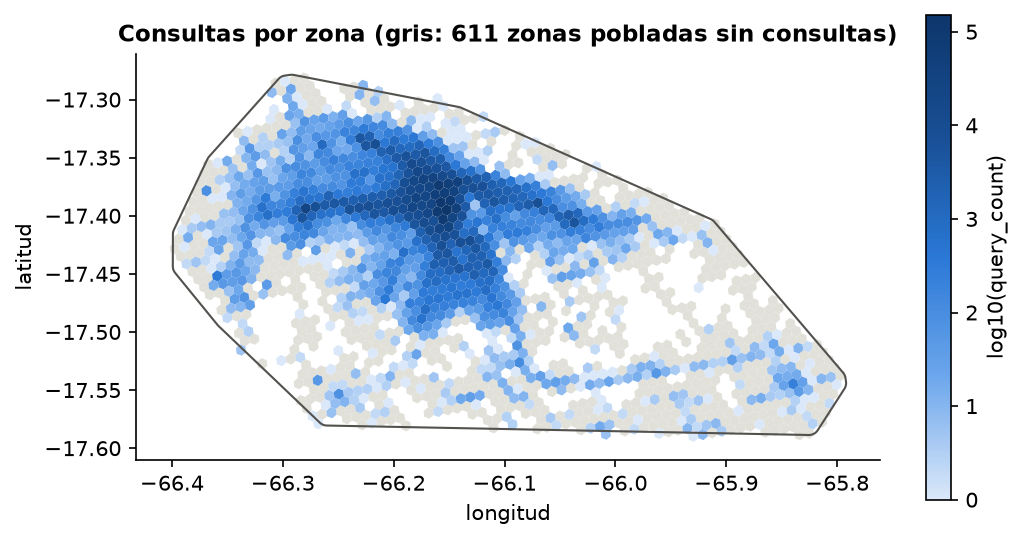
\includegraphics[width=0.85\textwidth]{imagenes/07_desarrollo/7_3_preparacion/consultas_por_zona.png}
  \fuente{Elaboración propia, a partir de \var{02_preprocesamiento} (sección 8). Escala de
  color: $\log_{10}$ del conteo; gris: zonas pobladas sin consultas.}
\end{figure}

Las zonas sin consultas no se distribuyen al azar: se concentran en la periferia del
valle y en el sur del área, lejos del núcleo donde el color es más intenso. Si se
eliminaran, la tabla describiría solo el territorio donde la aplicación ya se usa.

\textbf{Zonas del modelo.} De las 1.628 zonas, entran al modelo las que tienen al menos
10 habitantes, que son 1.381. La tabla~\ref{tab:zonas-modelo} muestra qué se excluye. El
motivo es técnico: el modelo estima una tasa por habitante, y con muy pocos habitantes esa
tasa se vuelve inestable (una sola consulta en una zona de 2 habitantes equivale a 500 por
cada 1.000). Las zonas sin población no pueden entrar, porque la exposición sería cero. La
exclusión apenas afecta al volumen: se pierden 242 consultas, y el modelo conserva
1.924.336 de las 1.924.578 consultas válidas (el 99,99~\%).

\begin{table}[H]
  \centering
  \caption{Zonas del área de estudio según su población}
  \label{tab:zonas-modelo}
  \interlineadoSimple
  \small
  \begin{tabular}{@{}lrr@{}}
    \toprule
    \textbf{Grupo} & \textbf{Zonas} & \textbf{Consultas} \\
    \midrule
    Sin población en Kontur (\var{population} $= 0$) & 43 & 102 \\
    Entre 1 y 9 habitantes & 204 & 140 \\
    \textbf{Al menos 10 habitantes (zonas del modelo)} & \textbf{1.381} & \textbf{1.924.336} \\
    \midrule
    Total & 1.628 & 1.924.578 \\
    \bottomrule
  \end{tabular}
  \fuente{Elaboración propia, a partir de
  \var{resultados/03_feature_engineering/zonas_por_grupo.csv}.}
\end{table}

La población total de las 1.628 zonas es de 1.226.308 habitantes, algo más que los
1.223.871 de las celdas de Kontur situadas dentro del área
(sección~\ref{sec:area-estudio}). La diferencia, de 2.437 habitantes, proviene de las
zonas de borde incorporadas por tener consultas: su centroide queda fuera del contorno,
pero Kontur les asigna población.

\subsection{Limpieza, datos faltantes y valores atípicos}
\label{sec:limpieza}

\textbf{Consolidación.} Los 85 archivos, que cubren 84 semanas con datos (una semana viene
partida en dos archivos; sección~\ref{sec:cobertura-temporal}), se leen con detección automática de codificación:
se intenta UTF-8 y, si falla, Latin-1. Así se leen correctamente los seis archivos del
lote 2024 y los nombres con tildes (por ejemplo, ``Santivañez''). Las columnas
equivalentes de ambos esquemas se unifican, y a cada fila se le añade su linaje. Las
consultas se ordenan de forma estable (archivo, marca de tiempo, usuario y coordenadas),
para que cualquier ejecución produzca exactamente el mismo resultado.

\textbf{Filtros.} Se aplican seis filtros en un orden fijo, que va de lo inequívoco a lo
que depende de decisiones. La tabla~\ref{tab:flujo-filtros} y la
figura~\ref{fig:flujo-limpieza} muestran cuántas consultas elimina cada paso.

\begin{table}[H]
  \centering
  \caption{Flujo de limpieza de las consultas}
  \label{tab:flujo-filtros}
  \interlineadoSimple
  \small
  \begin{tabularx}{\textwidth}{@{}clrrY@{}}
    \toprule
    \textbf{Paso} & \textbf{Regla} & \textbf{Eliminadas} & \textbf{Quedan} & \textbf{Justificación} \\
    \midrule
    0 & Consultas crudas & --- & 1.927.675 & --- \\
    1 & Origen en (0,0) & 3 & 1.927.672 & Coordenadas no localizables \\
    2 & Origen fuera de Bolivia & 9 & 1.927.663 & Coordenadas imposibles para el servicio \\
    3 & Copia de duplicado exacto & 60 & 1.927.603 & Se conserva la primera aparición \\
    4 & Origen fuera del área & 2.509 & 1.925.094 & Área fijada en la sección~\ref{sec:area-estudio} \\
    5 & Distancia $>$ 50~km & 283 & 1.924.811 & Fuera de la escala urbana (sección~\ref{sec:atipicos}) \\
    6 & Usuario anómalo & 233 & 1.924.578 & Al menos 2 de 6 señales (sección~\ref{sec:atipicos}) \\
    \bottomrule
  \end{tabularx}
  \fuente{Elaboración propia, a partir de
  \var{resultados/02_preprocesamiento/flujo_limpieza.csv}. Se conserva el 99,84~\% de las
  consultas.}
\end{table}

\begin{figure}[H]
  \centering
  \caption{Consultas eliminadas en cada paso de la limpieza}
  \label{fig:flujo-limpieza}
  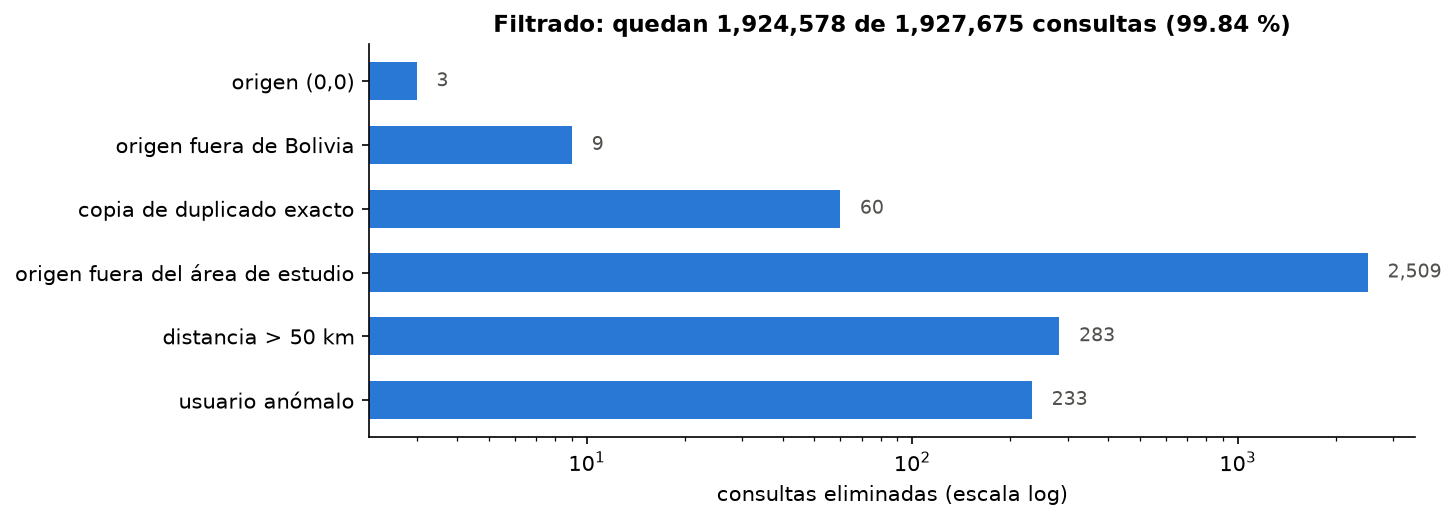
\includegraphics[width=0.9\textwidth]{imagenes/07_desarrollo/7_3_preparacion/flujo_limpieza.png}
  \fuente{Elaboración propia, a partir de \var{02_preprocesamiento} (sección 5). Eje
  horizontal en escala logarítmica.}
\end{figure}

El orden importa por dos motivos. Primero, los filtros geográficos inequívocos (pasos 1 y
2) van antes que la detección de duplicados, para que las coordenadas imposibles no
cuenten como consultas válidas. Segundo, el área de estudio (paso 4) se delimitó con los
orígenes de usuarios no anómalos y \emph{sin} aplicar el umbral de distancia, de modo que
los dos criterios no se contaminan entre sí. La mayor exclusión, la de consultas fuera del
área, representa apenas el 0,13~\% del total. En conjunto, la limpieza no altera la
estructura de los datos: corrige errores puntuales. Las cifras coinciden exactamente con
las que midió el análisis exploratorio, porque ambos notebooks usan las mismas funciones.

\textbf{Datos faltantes.} La limpieza no imputa ningún valor, por tres razones:
\begin{itemize}
  \item Las columnas que usa el proyecto no tienen nulos
        (sección~\ref{sec:datos-faltantes-eda}).
  \item Las 611 zonas pobladas sin consultas reciben un conteo de 0, que es su valor
        observado. No se trata como faltante.
  \item Las 43 zonas con consultas pero sin registro en Kontur reciben población 0. Es una
        ausencia estructural de la fuente, no un dato que deba estimarse; esas zonas quedan
        fuera del modelo por el umbral de población.
\end{itemize}
Las siete semanas sin datos tampoco se rellenan. Se registran para calcular las semanas
realmente observadas (sección~\ref{sec:transformaciones}).

\textbf{Valores atípicos.} Solo se eliminan los atípicos que representan errores o un uso
no humano: la distancia de más de 50~km y los usuarios anómalos. Los valores extremos
legítimos se conservan. Por ejemplo, la zona con más consultas acumula 152.494, frente a
una mediana de 6. Esas zonas son reales, están en el centro de la ciudad y forman parte
del fenómeno. Su efecto se controla con métricas y modelos propios de datos de conteo, no
eliminándolas.

\subsection{Transformaciones y codificación de variables}
\label{sec:transformaciones}

Las transformaciones convierten consultas individuales en un conjunto de datos H3 por zona y dejan cada
variable en la escala que requieren los modelos. La tabla~\ref{tab:transformaciones} las
resume con su justificación.

\begin{table}[H]
  \centering
  \caption{Transformaciones y codificación aplicadas}
  \label{tab:transformaciones}
  \interlineadoSimple
  \small
  \begin{tabularx}{\textwidth}{@{}L{0.26\textwidth}L{0.34\textwidth}Y@{}}
    \toprule
    \textbf{Transformación} & \textbf{Qué hace} & \textbf{Por qué} \\
    \midrule
    Asignación de zona & Convierte las coordenadas de origen en su celda H3 de resolución~8 (\var{h3_origin}) & Unidad de análisis común con Kontur, sin reproyección (sección~\ref{subsec:h3}) \\
    Agregación & Cuenta las consultas por zona de origen (\var{query_count}) & La variable objetivo es el total del período \\
    Bloque espacial & Asigna a cada zona su celda madre H3 de resolución~6 (\var{block_id}), de unos 36~km\textsuperscript{2} & Unidad de validación y de reserva de prueba \\
    Semanas equivalentes observadas & $W_{obs} = \text{días con datos} / 7 = 568/7 = 81{,}143$ & Expresar lo esperado por semana sin contar el hueco \\
    Exposición & $\log(\text{population})$ como \emph{offset} (coeficiente fijo igual a 1) & Modelar la tasa por habitante (sección~\ref{subsec:glm-poisson}) \\
    Escala de población & $\log(1 + x)$ en \var{pop_ring1} dentro de los modelos & Reduce la asimetría; no depende de los datos, así que no filtra información \\
    Municipio & Municipio más frecuente entre los orígenes de la zona; sin consultas, el de las zonas vecinas etiquetadas más cercanas & Estrato de la línea base B1 \\
    Anillo de distancia & Cuatro anillos (A1 a A4) según los cuartiles de la distancia media de cada bloque a la Plaza & Estrato de la línea base B2 y del sorteo de prueba \\
    \bottomrule
  \end{tabularx}
  \fuente{Elaboración propia, a partir de \var{src/features.py}, \var{src/modelos.py},
  \var{src/limpieza.py} y \var{resultados/02_preprocesamiento/metricas.json}.}
\end{table}

\textbf{Semanas equivalentes observadas ($W_{obs}$).} Hubo datos 538 días antes del hueco
y 30 después, 568 días en total, que equivalen a 81,143 semanas. Todos los modelos estiman
el total del período. Para comunicar el resultado a la organización en una unidad
intuitiva (consultas por semana), ese total se divide por $W_{obs}$ y no por las 91
semanas calendario. Dividir por 91 subestimaría el ritmo semanal, porque contaría semanas
en las que no se registró nada.

\textbf{Codificación de las variables categóricas.} El municipio y el anillo no se
convierten en variables indicadoras (\emph{one-hot}), porque ningún modelo los usa como
predictores. Sirven para definir los estratos de dos líneas base, que calculan una tasa
separada por grupo.

La etiqueta de municipio proviene del campo \var{origin_municipio} de las exportaciones de
Trufi Association, no de límites oficiales, y queda asignada a 14 municipios
(tabla~\ref{tab:municipios}). El municipio figura como ``Cochabamba'' en los datos, pero
corresponde a Cercado. Para comprobar si esa etiqueta es coherente dentro de cada zona, se
verificó su pureza. El 99,38~\% de las consultas comparte la etiqueta modal de su zona. Solo
el 5,02~\% de las zonas con consultas es de municipio \emph{mixto}, es decir, tiene menos
del 90~\% de sus consultas con la etiqueta modal. El único caso llamativo, Arani (50~\%),
corresponde a una zona con apenas dos consultas.

Esta decisión es aceptable para el propósito del proyecto porque el municipio se usa
únicamente como estrato en la línea base B1, que no fue la técnica seleccionada; ningún
modelo que participa en la selección final lo usa como predictor. Los resultados se
guardan en \var{resultados/03_feature_engineering/resumen_municipio.csv} y en
\var{metricas.json} (\var{pct_consultas_municipio_modal},
\var{pct_zonas_municipio_mixto}).

\begin{table}[H]
  \centering
  \caption{Zonas del modelo por municipio asignado y pureza de la etiqueta}
  \label{tab:municipios}
  \interlineadoSimple
  \small
  \begin{tabular}{@{}lrrrrr@{}}
    \toprule
    \textbf{Municipio} & \textbf{Zonas} & \textbf{Consultas} & \textbf{Población} & \textbf{\celda{\% consultas con\\etiqueta modal}} & \textbf{\celda{Zonas\\mixtas}} \\
    \midrule
    Cochabamba (Cercado) & 318 & 1.662.310 & 622.120 & 99,69 & 13 \\
    Sacaba & 259 & 90.113 & 180.427 & 99,99 & 1 \\
    Quillacollo & 137 & 65.275 & 146.291 & 97,71 & 12 \\
    Colcapirhua & 35 & 53.209 & 47.652 & 97,17 & 5 \\
    Tiquipaya & 47 & 46.785 & 60.991 & 92,27 & 7 \\
    Vinto & 89 & 3.403 & 56.167 & 95,53 & 4 \\
    Sipe Sipe & 92 & 1.357 & 35.950 & 99,78 & 2 \\
    Arbieto & 86 & 546 & 17.368 & 97,99 & 1 \\
    Villa Punata & 74 & 488 & 23.430 & 100,00 & 0 \\
    Tolata & 37 & 302 & 5.115 & 100,00 & 0 \\
    Villa Santivañez & 79 & 300 & 4.163 & 100,00 & 0 \\
    Villa José Quintín Mendoza & 76 & 170 & 13.386 & 99,41 & 1 \\
    Cliza & 47 & 76 & 11.604 & 100,00 & 0 \\
    Arani & 5 & 2 & 1.015 & 50,00 & 1 \\
    \midrule
    Total & 1.381 & 1.924.336 & 1.225.679 & 99,38 & 47 \\
    \bottomrule
  \end{tabular}
  \fuente{Elaboración propia, a partir de
  \var{resultados/03_feature_engineering/resumen_municipio.csv} y \var{metricas.json}. Zona
  mixta: menos del 90~\% de sus consultas con la etiqueta modal.}
\end{table}

La tabla muestra por qué el área de estudio excede los siete municipios del eje
metropolitano mencionados en el alcance. La componente contigua de orígenes se extiende
hacia el valle alto y el sur (Arbieto, Santivañez, Punata, Cliza, Tolata). Esos
municipios aportan muchas zonas pobladas, pero casi ninguna consulta. Cercado concentra el
86~\% de las consultas con el 51~\% de la población.

\subsection{Ingeniería y selección de características}
\label{sec:ingenieria-caracteristicas}

Cada columna del conjunto de datos H3 tiene un papel declarado antes de modelar. La
tabla~\ref{tab:grupos-variables} organiza las variables por su uso. Distinguir estos
papeles es la principal salvaguarda contra la fuga de información
(sección~\ref{subsec:fuga-datos}).

\begin{table}[H]
  \centering
  \caption{Variables del conjunto de datos H3 según su papel}
  \label{tab:grupos-variables}
  \interlineadoSimple
  \small
  \begin{tabularx}{\textwidth}{@{}L{0.18\textwidth}L{0.28\textwidth}Y@{}}
    \toprule
    \textbf{Papel} & \textbf{Variables} & \textbf{Uso} \\
    \midrule
    Objetivo & \var{query_count} & Lo que se estima: total de consultas de la zona en el período \\
    Exposición & \var{population} & Entra como \emph{offset} $\log(\text{population})$: convierte el conteo en una tasa por habitante \\
    Predictores & \var{dist_centro_km}, \var{pop_ring1} & Únicas variables explicativas de los modelos M1 a M3 \\
    Contraste & \var{dist_trazado_m}, \var{gtfs_covered} & Solo para interpretar la brecha; nunca entran a un modelo \\
    Grupos y validación & \var{municipality}, \var{distance_ring}, \var{block_id}, \var{in_test} & Estratos de las líneas base, pliegues de validación y marca de prueba \\
    Apoyo & \var{h3_cell}, \var{lat}, \var{lon}, \var{in_model}, \var{user_count}, conteos antes y después del hueco & Identificación, mapas, universo del modelo y análisis de sensibilidad \\
    \bottomrule
  \end{tabularx}
  \fuente{Elaboración propia, a partir de \var{config.py} (\var{PREDICTORES},
  \var{CONTRASTE}) y \var{03_feature_engineering} (secciones 3 a 7).}
\end{table}

La construcción de las variables sigue cuatro decisiones:

\textbf{Centro de referencia exógeno.} La distancia al centro (\var{dist_centro_km}) se
mide como distancia geodésica desde el centroide de cada zona hasta la Plaza 14 de
Septiembre, un punto fijado desde fuera de los datos. Como se vio en la
sección~\ref{sec:relaciones-variables}, este centro se asocia con las consultas mucho más
que el centroide del área. Tiene además una ventaja metodológica: al no calcularse con los
datos, no cambia entre pliegues de validación ni puede filtrar información de las zonas de
prueba.

\textbf{Población del entorno.} \var{pop_ring1} suma la población de las seis zonas del
primer anillo H3 alrededor de cada zona, sin incluirla a ella. \var{pop_ring2} hace lo
mismo con el segundo anillo. Ambas se calculan con la cobertura completa de Kontur para
Bolivia, y no solo con el área de estudio. Así, las zonas de borde no ven su entorno
artificialmente vacío. Estas variables capturan la densidad del vecindario, un indicador
indirecto de la concentración de actividades.

\textbf{Selección por colinealidad.} La figura~\ref{fig:correlacion-predictores} muestra
la correlación de Spearman entre los predictores candidatos. \var{pop_ring1} y
\var{pop_ring2} tienen una correlación de 0,954: aportan prácticamente la misma
información, e incluir ambas inflaría la varianza de los coeficientes sin mejorar la
estimación. Se conserva \var{pop_ring1}, que describe el entorno más inmediato y se asocia
un poco más con el conteo (0,836 frente a 0,804). La población de la propia zona no
aparece como predictor porque ya entra como exposición.

\begin{figure}[H]
  \centering
  \caption{Correlación de Spearman entre los predictores candidatos}
  \label{fig:correlacion-predictores}
  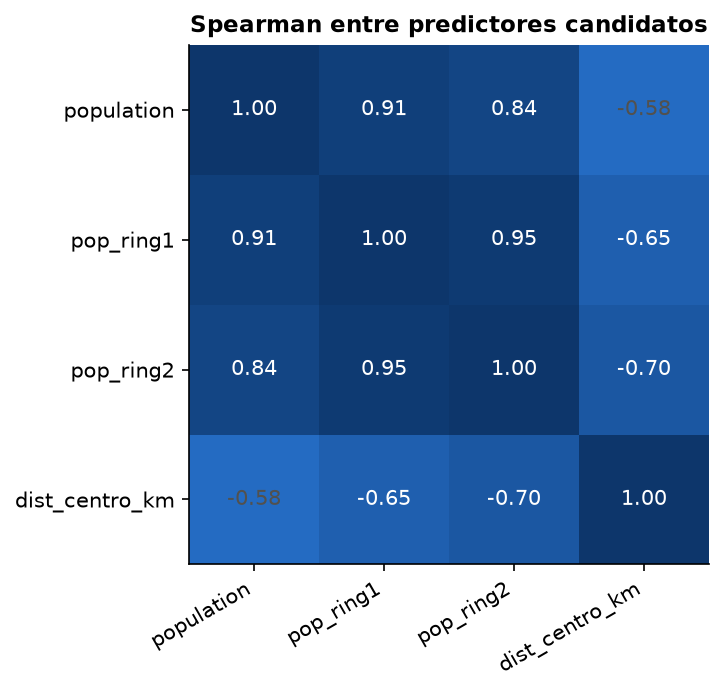
\includegraphics[width=0.5\textwidth]{imagenes/07_desarrollo/7_3_preparacion/correlacion_predictores.png}
  \fuente{Elaboración propia, a partir de
  \var{resultados/03_feature_engineering/correlacion_predictores.csv}.}
\end{figure}

\textbf{Exclusión de la cobertura.} \var{dist_trazado_m} es la distancia del centroide de
la zona al trazado GTFS más cercano, calculada en proyección métrica UTM 19S.
\var{gtfs_covered} vale 1 si esa distancia es de 500~m o menos. Con ese criterio, 634 de
las 1.628 zonas están cubiertas (626 de las 1.381 zonas del modelo). Ambas variables se
excluyen expresamente de los predictores
(secciones~\ref{sec:traduccion-necesidad} y~\ref{sec:area-estudio}), y el notebook de
modelado verifica que ninguna técnica las use. La cobertura se mide contra el trazado y no
contra las paradas, por la naturaleza del paratránsito (sección~\ref{subsec:gtfs}).

Con estas decisiones, el conjunto de predictores queda reducido a dos variables:
\var{dist_centro_km}, que resume la localización, y \var{pop_ring1}, que resume el
entorno. Es un conjunto deliberadamente pequeño. Con 1.381 zonas y una autocorrelación
fuerte, el número efectivo de observaciones independientes es mucho menor que el nominal,
y cada predictor adicional aumenta el riesgo de sobreajuste. Además, ambas variables son
exógenas: ninguna se calcula a partir de las consultas.

\subsection{Conjuntos de entrenamiento y prueba}
\label{sec:conjuntos-entrenamiento-prueba}

El conjunto de prueba se reserva en esta fase, antes de ajustar cualquier modelo, y se usa
una sola vez en la evaluación. La reserva no se hace por zonas individuales sino por
\emph{bloques} H3 de resolución~6: por la autocorrelación documentada en la
sección~\ref{sec:relaciones-variables}, una zona de prueba rodeada de vecinas de
entrenamiento sería casi una copia de ellas, y el error medido resultaría optimista
(sección~\ref{subsec:validacion-espacial}).

Las 1.381 zonas del modelo se reparten en 53 bloques. Para que la prueba represente todo el
gradiente centro-periferia, el sorteo se estratifica por anillo de distancia: en cada
anillo se reserva el 20~\% de sus bloques, con la semilla fija 42. Los cortes entre anillos
(12,52, 18,65 y 22,92~km de la Plaza) son los cuartiles de la distancia media de los
bloques, de modo que cada anillo tiene un número parecido de bloques. El sorteo solo usa la
geometría de los bloques y su anillo: ninguna consulta interviene en la selección.

\begin{table}[H]
  \centering
  \caption{Zonas del modelo por anillo de distancia}
  \label{tab:anillos}
  \interlineadoSimple
  \small
  \begin{tabular}{@{}lrrrrrr@{}}
    \toprule
    \textbf{Anillo} & \textbf{\celda{Distancia\\a la Plaza (km)}} & \textbf{Bloques} & \textbf{\celda{Bloques\\de prueba}} & \textbf{Zonas} & \textbf{Consultas} & \textbf{\celda{Consultas por\\1.000 hab.}} \\
    \midrule
    A1 & hasta 12,52 & 14 & 3 & 501 & 1.854.930 & 2.139,9 \\
    A2 & 12,52 a 18,65 & 13 & 3 & 342 & 66.102 & 303,5 \\
    A3 & 18,65 a 22,92 & 13 & 3 & 234 & 2.251 & 31,9 \\
    A4 & más de 22,92 & 13 & 3 & 304 & 1.053 & 14,9 \\
    \midrule
    Total & & 53 & 12 & 1.381 & 1.924.336 & 1.570,0 \\
    \bottomrule
  \end{tabular}
  \fuente{Elaboración propia, a partir de
  \var{resultados/03_feature_engineering/resumen_anillo.csv} y \var{test_blocks.csv}.}
\end{table}

La tabla~\ref{tab:particion} y la figura~\ref{fig:anillos-prueba} muestran el resultado.
La prueba reúne 12 bloques y 352 zonas (el 25,5~\% de las zonas), pero solo el 9,63~\% de
las consultas.

\begin{table}[H]
  \centering
  \caption{Partición en entrenamiento y prueba por bloques espaciales}
  \label{tab:particion}
  \interlineadoSimple
  \small
  \begin{tabular}{@{}lrrrrr@{}}
    \toprule
    \textbf{Conjunto} & \textbf{Bloques} & \textbf{Zonas} & \textbf{Consultas} & \textbf{Población} & \textbf{\celda{Consultas por\\1.000 hab.}} \\
    \midrule
    Entrenamiento & 41 & 1.029 & 1.738.942 & 908.744 & 1.913,6 \\
    Prueba & 12 & 352 & 185.394 & 316.935 & 585,0 \\
    \bottomrule
  \end{tabular}
  \fuente{Elaboración propia, a partir de
  \var{resultados/03_feature_engineering/particion.csv}.}
\end{table}

\begin{figure}[H]
  \centering
  \caption{Anillos de distancia al centro y bloques reservados como prueba}
  \label{fig:anillos-prueba}
  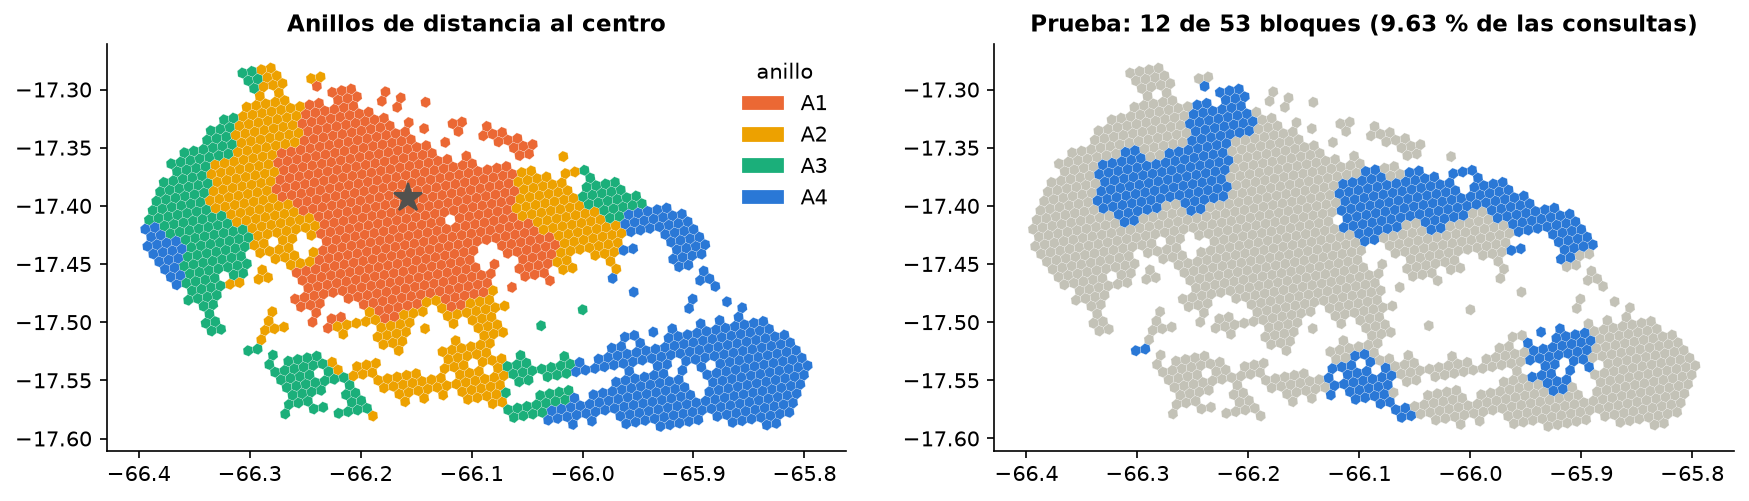
\includegraphics[width=\textwidth]{imagenes/07_desarrollo/7_3_preparacion/anillos_y_prueba.png}
  \fuente{Elaboración propia, a partir de \var{03_feature_engineering} (secciones 8 y 10).
  Izquierda: anillos A1 a A4 (la estrella marca la Plaza 14 de Septiembre); derecha: bloques
  de prueba en azul.}
\end{figure}

El desequilibrio entre zonas y consultas tiene una explicación, y debe tenerse en cuenta
al leer la evaluación. Los bloques del núcleo central, donde se concentra la mayor parte de
las consultas, quedaron del lado de entrenamiento. Por eso la tasa de la prueba (585
consultas por cada 1.000 habitantes) es un tercio de la de entrenamiento (1.913,6). La
prueba es, por tanto, más periférica y menos intensa que el conjunto con el que se
entrena. Es una condición exigente pero realista: la organización necesita estimaciones
confiables justamente en zonas alejadas del centro. Además, 125 de las 352 zonas de prueba
tocan zonas de entrenamiento en el borde de su bloque
(\var{zonas_prueba_borde} en \var{resultados/03_feature_engineering/metricas.json}). Es una
fuga mínima e inevitable en cualquier partición espacial, que se documenta y no se oculta.

El notebook termina con cuatro verificaciones automáticas:
\begin{itemize}
  \item la tabla conserva todas las consultas y no tiene nulos;
  \item los rangos de las variables son válidos;
  \item entrenamiento y prueba no comparten ningún bloque;
  \item ni el objetivo ni las variables GTFS figuran entre los predictores.
\end{itemize}
Los bloques reservados se guardan en \var{test_blocks.csv}. A partir de aquí, el notebook
de modelado solo los descarta y el de evaluación los usa una única vez.

% ============================================================
%  7.4. MODELADO  -- parte del capítulo 7
%  ------------------------------------------------------------
%  Guía 2.7.4: (1) tipo de problema, (2) algoritmos, (3) por qué,
%  (4) entrenamiento, (5) parámetros e hiperparámetros,
%  (6) comparación de alternativas, (7) no presentar un modelo
%  como mejor solo por ser el primero ejecutado.
%  Notebook: 04_modelado.ipynb   Código: src/modelos.py
%  Cifras:   resultados/04_modelado/ (metricas.json, cv_resumen.csv,
%            cv_por_pliegue.csv, regla_seleccion.csv, coeficientes.csv)
% ============================================================
\section{Modelado}
\label{sec:modelado}

El modelado elige la técnica con la que se calcula el conteo esperado de cada zona. Se
ejecuta en el notebook \var{04_modelado} y trabaja solo con las 1.029 zonas de
entrenamiento, repartidas en 41 bloques. Las 352 zonas de prueba se descartan al cargar
los datos y no intervienen en ninguna decisión de esta fase. El protocolo completo, que
incluye las técnicas, los predictores, los pliegues de validación y la regla de selección,
se escribió en \var{config.py} y se registró en el control de versiones antes de ejecutar
el primer modelo.

\subsection{Tipo de problema analítico}
\label{sec:tipo-problema}

Se trata de un problema de \textbf{regresión supervisada sobre datos de conteo con
exposición}, en un corte transversal:
\begin{itemize}
  \item Es \emph{supervisado} porque para cada zona de entrenamiento se conoce el valor
        observado de la variable objetivo, \var{query_count}.
  \item Es una \emph{regresión} porque se estima una cantidad, el número esperado de
        consultas, y no una categoría.
  \item Es un problema de \emph{conteo} porque el objetivo es un entero no negativo, con
        muchos ceros, fuertemente asimétrico y sobredisperso
        (sección~\ref{sec:distribucion-objetivo}). Por eso los errores se miden con la
        devianza de Poisson y no con el error cuadrático (sección~\ref{subsec:devianza-poisson}).
  \item Tiene \emph{exposición} porque, a igualdad de condiciones, el conteo debe crecer en
        proporción a la población. Todas las técnicas estiman, en el fondo, una
        \emph{tasa} de consultas por habitante, que luego se multiplica por la población de
        la zona.
  \item Es \emph{transversal} porque cada zona aporta una sola observación, el total del
        período, y el tiempo no interviene.
\end{itemize}

La predicción se usa de una forma particular: no interesa acertar el conteo de las zonas
de entrenamiento, que ya se conoce, sino obtener para \emph{cada} zona un valor esperado
calculado sin que la zona se vea a sí misma. Ese valor es el que después se compara con lo
observado para medir la brecha (sección~\ref{sec:interpretacion-resultados}).

\subsection{Selección de algoritmos}
\label{sec:seleccion-algoritmos}

Se compararon siete técnicas, ordenadas de menor a mayor complejidad en lo que en este
trabajo se denomina \emph{escalera}. Cada técnica se identifica con un código de letra y
número, que se usa tal cual en el código fuente, los resultados y las figuras:

\begin{itemize}
  \item La letra \textbf{B} viene de \emph{baseline}, que en español se traduce como
    \textbf{línea base}: un \emph{punto de referencia inicial}, es decir, una estimación
    deliberadamente simple que cualquier técnica más elaborada debe superar para justificar
    su complejidad. Las cuatro líneas base (B0 a B3) no ajustan parámetros por optimización.
    Calculan una tasa de consultas por habitante con una regla aritmética y la multiplican
    por la población de la zona.
  \item La letra \textbf{M} viene de \emph{modelo}. Designa las tres técnicas (M1 a M3) que
    estiman parámetros optimizando una función de pérdida o de verosimilitud a partir de
    los predictores \var{dist_centro_km} y \var{pop_ring1}.
  \item El \textbf{número} indica la posición en la escalera: B0 es la más simple y M3 la
    más compleja. Cuando dos técnicas empatan en desempeño, la regla de selección elige la
    de número menor (sección~\ref{sec:regla-seleccion}).
\end{itemize}

La tabla~\ref{tab:escalera-tecnicas} resume las siete técnicas. En todas las fórmulas,
$Y_i$ es el conteo observado de la zona~$i$, $P_i$ su población y $\hat{\mu}_i$ su conteo
esperado. Las sumas se calculan solo sobre zonas de entrenamiento.

\begin{table}[H]
  \centering
  \caption{Escalera de técnicas: códigos, cálculo del esperado y fundamento}
  \label{tab:escalera-tecnicas}
  \interlineadoSimple
  \small
  \begin{tabularx}{\textwidth}{@{}L{0.07\textwidth}L{0.20\textwidth}YL{0.11\textwidth}@{}}
    \toprule
    \textbf{Código} & \textbf{Nombre} & \textbf{Cómo calcula el conteo esperado de una zona} & \textbf{Marco} \\
    \midrule
    B0 & Tasa global & Tasa única de todo el entrenamiento: $\hat{\mu}_i = P_i \cdot \sum Y / \sum P$ & \ref{subsec:lineas-base} \\
    B1 & Tasa por municipio & Tasa del municipio de la zona; si el municipio no está en el entrenamiento, tasa global & \ref{subsec:lineas-base} \\
    B2 & Tasa por anillo & Tasa del anillo de distancia (A1 a A4) de la zona & \ref{subsec:lineas-base} \\
    B3 & Vecindad H3 & Tasa conjunta de las zonas de entrenamiento más cercanas (al menos 3, sin la propia zona) & \ref{subsec:suavizado-vecindad} \\
    M1 & Poisson con \emph{offset} & $\log \hat{\mu}_i = \log P_i + \beta_0 + \beta_1\,d_i + \beta_2 \log(1 + R_i)$, por máxima verosimilitud & \ref{subsec:glm-poisson} \\
    M2 & Binomial negativa NB2 & Igual que M1, con varianza $\mu + \alpha\mu^2$; $\alpha$ se estima con los datos & \ref{subsec:binomial-negativa} \\
    M3 & \emph{Gradient boosting} con pérdida de Poisson & Suma de árboles de decisión sobre $d_i$ y $\log(1+R_i)$, ajustados a la tasa $Y_i/P_i$ con peso $P_i$ & \ref{subsec:gradient-boosting} \\
    \bottomrule
  \end{tabularx}
  \fuente{Elaboración propia, a partir de \var{src/modelos.py} y \var{config.py}. $d_i$:
  \var{dist_centro_km}; $R_i$: \var{pop_ring1}.}
\end{table}

A continuación se explica cada técnica en palabras, tal como está implementada.

\textbf{B0, tasa global.} Supone que todas las zonas tienen la misma propensión a
consultar y que solo difieren en población. Suma las consultas de todas las zonas de
entrenamiento, las divide por su población total y aplica esa tasa única a cada zona. Es
el punto de referencia principal del proyecto (sección~\ref{subsec:modelo-referencia}): si
ninguna técnica lo supera, el contexto territorial no aporta nada más allá de la
población, y la brecha sería una simple comparación de tasas brutas.

\textbf{B1, tasa por municipio.} Calcula una tasa separada para cada municipio con las
zonas de entrenamiento de ese municipio y la aplica a las zonas del mismo municipio.
Representa la hipótesis de que la propensión a consultar cambia de un municipio a otro,
por ejemplo por diferencias de adopción o de cobertura cartográfica. Si una zona pertenece
a un municipio sin zonas de entrenamiento, recibe la tasa global.

\textbf{B2, tasa por anillo.} Hace lo mismo que B1, pero con los cuatro anillos de
distancia a la Plaza. Representa el gradiente centro-periferia de la economía urbana
(sección~\ref{subsec:lineas-base}).

\textbf{B3, vecindad H3.} Estima la tasa de una zona con la tasa conjunta de sus vecinas de
entrenamiento más cercanas. El procedimiento tiene tres pasos:
\begin{enumerate}
  \item Se buscan zonas de entrenamiento en el primer anillo H3 alrededor de la zona, sin
        incluirla a ella.
  \item Si hay menos de tres, se amplía la búsqueda al segundo anillo, luego al tercero, y
        así hasta un máximo de diez anillos.
  \item Con las vecinas encontradas se calcula $\sum Y_j / \sum P_j$, y ese cociente se
        multiplica por la población de la zona. Si ni siquiera a diez anillos hay tres
        vecinas de entrenamiento, se usa la tasa global.
\end{enumerate}
El umbral de tres vecinas (\var{VECINAS_MIN}) evita que la tasa dependa de una sola zona
vecina. El límite de diez anillos (\var{K_VECINDAD_MAX}), unos 9~km, impide usar zonas
demasiado lejanas. B3 aprovecha directamente la autocorrelación espacial hallada en la
sección~\ref{sec:relaciones-variables}. No estima coeficientes: su ``ajuste'' consiste en
memorizar los conteos y las poblaciones de entrenamiento, como un estimador de vecinos
cercanos. Como la zona nunca entra en su propio cálculo, el esperado de B3 no puede copiar
el valor observado.

\textbf{M1, regresión de Poisson con offset.} Es un modelo lineal generalizado con enlace
logarítmico. El término $\log P_i$ entra con coeficiente fijo igual a 1 (\emph{offset}),
de modo que el modelo describe cómo varía la \emph{tasa} por habitante con la distancia al
centro y con la población del entorno. Los coeficientes se estiman por máxima
verosimilitud. La relación es multiplicativa: cada kilómetro de distancia multiplica la
tasa por $e^{\beta_1}$. M1 supone que la varianza del conteo es igual a su media.

\textbf{M2, binomial negativa NB2.} Mantiene la misma ecuación para la media que M1, pero
permite que la varianza crezca más rápido que la media, según $\mu + \alpha\mu^2$. El
parámetro de sobredispersión $\alpha$ se estima con los datos: si $\alpha = 0$, M2 se
reduce a M1. Responde al hallazgo de que la varianza es decenas de miles de veces la media
(sección~\ref{sec:distribucion-objetivo}).

\textbf{M3, gradient boosting con pérdida de Poisson.} Construye una suma de árboles de
decisión, cada uno de los cuales corrige los errores de los anteriores. Así captura
relaciones no lineales e interacciones entre la distancia y la población del entorno sin
especificarlas de antemano. La implementación usada no admite \emph{offset}, así que se
modela la tasa $Y_i/P_i$ ponderando cada zona por su población, una formulación
equivalente en esperanza (sección~\ref{subsec:gradient-boosting}). Sus hiperparámetros se
eligen con una validación interna, descrita en la sección~\ref{sec:hiperparametros}.

\subsection{Justificación de la selección}
\label{sec:justificacion-algoritmos}

Las siete técnicas no se eligieron por exhaustividad, sino para que cada peldaño ponga a
prueba \emph{una} hipótesis adicional sobre qué determina las consultas esperadas. La
tabla~\ref{tab:hipotesis-escalera} explicita esa lógica y el hallazgo de la
sección~\ref{sec:comprension-datos} que motiva cada peldaño.

\begin{table}[H]
  \centering
  \caption{Hipótesis que pone a prueba cada peldaño de la escalera}
  \label{tab:hipotesis-escalera}
  \interlineadoSimple
  \small
  \begin{tabularx}{\textwidth}{@{}L{0.08\textwidth}YL{0.33\textwidth}@{}}
    \toprule
    \textbf{Código} & \textbf{Hipótesis que añade} & \textbf{Hallazgo que la motiva} \\
    \midrule
    B0 & La población basta para explicar las consultas & Spearman de 0,855 entre conteo y población \\
    B1 & La tasa difiere entre municipios & Cercado: 86~\% de las consultas con 51~\% de la población \\
    B2 & La tasa decae con la distancia al centro & Spearman de $-0{,}68$ entre tasa y distancia \\
    B3 & Zonas cercanas tienen tasas parecidas & $I$ de Moran de 0,72 entre vecinas \\
    M1 & La tasa varía de forma continua con la distancia y el entorno & Asociación de la tasa con \var{pop_ring1} y \var{dist_centro_km} \\
    M2 & Además, la varianza excede a la media & Varianza 46.569 veces la media \\
    M3 & Además, la relación es no lineal o tiene interacciones & Dispersión grande entre zonas de población similar \\
    \bottomrule
  \end{tabularx}
  \fuente{Elaboración propia, a partir de las secciones~\ref{sec:distribucion-objetivo}
  y~\ref{sec:relaciones-variables}.}
\end{table}

Ordenar las técnicas de esta forma permite interpretar la comparación. Si un peldaño mejora
claramente al anterior, su hipótesis aporta información. Si no lo mejora, la complejidad
añadida no se justifica. Incluir líneas base simples no es un trámite: en datos con
autocorrelación fuerte y pocas unidades independientes, un estimador local sencillo puede
competir con modelos más elaborados, y solo compararlos en las mismas condiciones permite
saberlo.

La escalera tampoco incluye bosques aleatorios u otras variantes de \emph{boosting}: M3
representa a la familia de conjuntos de árboles, y M2 a la de modelos que relajan el
supuesto de Poisson.

Tampoco se incluyeron modelos con exceso de ceros (ZIP y ZINB), pese a estar mencionados en
la sección~\ref{subsec:binomial-negativa}. La razón es empírica y la muestra la
tabla~\ref{tab:ceros-esperados}: en entrenamiento hay 345 ceros observados. El modelo de
Poisson espera 631,5, casi el doble; la binomial negativa espera 323,8, prácticamente los
observados (razón de 0,94). En otras palabras, una vez corregida la sobredispersión no queda
un exceso de ceros que modelar.

\begin{table}[H]
  \centering
  \caption{Ceros observados y esperados en las zonas de entrenamiento}
  \label{tab:ceros-esperados}
  \interlineadoSimple
  \small
  \begin{tabular}{@{}lrrrr@{}}
    \toprule
    \textbf{Técnica} & \textbf{\celda{Ceros\\observados}} & \textbf{\celda{Ceros\\esperados}} & \textbf{\celda{Esperados /\\observados}} & \textbf{\celda{Zonas con\\$\hat{\mu} < 0{,}5$}} \\
    \midrule
    B3 vecindad H3 & 345 & --- & --- & 179 \\
    M1 Poisson & 345 & 631,5 & 1,83 & 625 \\
    M2 binomial negativa & 345 & 323,8 & 0,94 & 89 \\
    \bottomrule
  \end{tabular}
  \fuente{Elaboración propia, a partir de \var{resultados/04_modelado/ceros_esperados.csv}
  (1.029 zonas de entrenamiento). B3 no define una distribución de probabilidad, por lo que
  no tiene ceros esperados.}
\end{table}

Los ceros del proyecto son, en su mayoría, muestrales y no estructurales. Son zonas
pobladas donde el evento no se observó, pero donde podría ocurrir si la aplicación
ofreciera información útil. Modelarlos con un proceso aparte absorbería justamente la señal
que el proyecto busca interpretar como brecha. Además, M2, que corrige la sobredispersión,
no fue seleccionada por la regla de un error estándar
(sección~\ref{sec:regla-seleccion}), de modo que un ZIP no tendría base empírica para
justificar su complejidad adicional.

\subsection{Proceso de entrenamiento}
\label{sec:proceso-entrenamiento}

Las siete técnicas se entrenan y comparan con una \textbf{validación cruzada espacial por
bloques}. Los 41 bloques de entrenamiento se reparten en cinco pliegues con
\var{GroupKFold}, un procedimiento que asigna cada bloque \emph{entero} a un solo pliegue.
Cada pliegue reúne entre 205 y 207 zonas. El proceso se repite cinco veces:
\begin{enumerate}
  \item Se toman cuatro pliegues como entrenamiento y el quinto como validación.
  \item Cada técnica se ajusta solo con los cuatro pliegues de entrenamiento. Todo lo que
        se estima (tasas, coeficientes, $\alpha$ e hiperparámetros) ocurre dentro de ese
        ajuste.
  \item Cada técnica predice las zonas del pliegue de validación, que no ha visto.
  \item Se calculan las métricas de ese pliegue.
\end{enumerate}

Al terminar, cada zona de entrenamiento tiene una predicción \emph{fuera de pliegue} por
cada técnica, calculada por un modelo que no la vio. La validación replica así la situación
real de uso, que es estimar zonas cuyas consultas no se conocen. Como los pliegues se forman
por bloques de unos 36~km\textsuperscript{2}, una zona de validación no tiene vecinas
inmediatas en el entrenamiento salvo en el borde de su bloque. Esto importa especialmente
para B3, que de otro modo tomaría la tasa de vecinas casi idénticas.

Una vez aplicada la regla de selección, la técnica elegida se ajusta con las 1.029 zonas
de entrenamiento y se guarda (\var{modelo_final.joblib}). Ese modelo final es el único que
se aplica a la prueba (sección~\ref{sec:evaluacion-resultados}).

El notebook termina con tres verificaciones:
\begin{itemize}
  \item ninguna zona de prueba intervino en la validación;
  \item cada zona de entrenamiento se predijo exactamente una vez por técnica, con bloques
        completos;
  \item los predictores usados son solo \var{dist_centro_km} y \var{pop_ring1}.
\end{itemize}

\subsection{Parámetros e hiperparámetros}
\label{sec:hiperparametros}

La tabla~\ref{tab:parametros-protocolo} reúne los parámetros del protocolo. Todos se
fijaron antes de modelar y ninguno se ajustó después de ver los resultados.

\begin{table}[H]
  \centering
  \caption{Parámetros del protocolo de modelado}
  \label{tab:parametros-protocolo}
  \interlineadoSimple
  \small
  \begin{tabularx}{\textwidth}{@{}L{0.30\textwidth}L{0.17\textwidth}Y@{}}
    \toprule
    \textbf{Parámetro (\var{config.py})} & \textbf{Valor} & \textbf{Significado} \\
    \midrule
    \var{PLIEGUES} & 5 & Pliegues de la validación cruzada por bloque \\
    \var{TOLERANCIA_EE} & 1,0 & Tolerancia de la regla de selección, en errores estándar \\
    \var{VECINAS_MIN} & 3 & B3: mínimo de zonas vecinas de entrenamiento \\
    \var{K_VECINDAD_MAX} & 10 & B3: anillo H3 máximo antes de usar la tasa global \\
    \var{GRILLA_GB} & 8 combinaciones & M3: profundidad máxima $\in \{3, \text{sin límite}\}$; mínimo de zonas por hoja $\in \{20, 50\}$; tasa de aprendizaje $\in \{0{,}05;\ 0{,}1\}$ \\
    \var{PLIEGUES_INTERNOS_GB} & 3 & M3: pliegues por bloque de la validación interna \\
    Iteraciones de M3 & hasta 300 & Con parada temprana \\
    \var{SEMILLA} & 42 & Semilla única del proyecto \\
    \bottomrule
  \end{tabularx}
  \fuente{Elaboración propia, a partir de \var{config.py} y \var{src/modelos.py}.}
\end{table}

\textbf{Hiperparámetros de M3.} M3 es la única técnica con hiperparámetros propiamente
dichos, y se eligen mediante \emph{validación anidada}. Dentro del ajuste de cada pliegue
externo, sus zonas de entrenamiento se dividen a su vez en tres pliegues internos por
bloque. Para cada una de las ocho combinaciones de la grilla se calcula la devianza media
interna, y se elige la menor. Así, la elección de hiperparámetros nunca ve el pliegue
externo de validación.

Los hiperparámetros elegidos por M3 en cada pliegue quedan registrados en
\var{cv_hiperparametros_m3.csv} (tabla~\ref{tab:hiperparametros-m3}). En el ajuste
completo sobre las 1.029 zonas de entrenamiento, la combinación elegida es: profundidad sin
límite, al menos 20 zonas por hoja y tasa de aprendizaje de 0,05, con 83 iteraciones tras
la parada temprana.

\begin{table}[H]
  \centering
  \caption{Hiperparámetros elegidos por M3 en cada pliegue y en el ajuste completo}
  \label{tab:hiperparametros-m3}
  \interlineadoSimple
  \small
  \begin{tabular}{@{}lrrrrr@{}}
    \toprule
    \textbf{Ajuste} & \textbf{\celda{Profundidad\\máxima}} & \textbf{\celda{Mínimo de\\zonas por hoja}} & \textbf{\celda{Tasa de\\aprendizaje}} & \textbf{Iteraciones} & \textbf{\celda{Devianza\\interna}} \\
    \midrule
    Pliegue 0 & 3 & 50 & 0,10 & 63 & 2.828,6 \\
    Pliegue 1 & 3 & 20 & 0,10 & 57 & 2.221,9 \\
    Pliegue 2 & 3 & 20 & 0,10 & 30 & 1.449,9 \\
    Pliegue 3 & 3 & 20 & 0,10 & 78 & 2.266,7 \\
    Pliegue 4 & sin límite & 20 & 0,10 & 33 & 2.389,4 \\
    \midrule
    Ajuste completo & sin límite & 20 & 0,05 & 83 & 2.172,3 \\
    \bottomrule
  \end{tabular}
  \fuente{Elaboración propia, a partir de
  \var{resultados/04_modelado/cv_hiperparametros_m3.csv} y \var{metricas.json}
  (\var{m3_*}). Devianza interna: media de los tres pliegues internos de la combinación
  elegida.}
\end{table}

La tabla muestra que la combinación elegida no es estable. En cuatro de los cinco pliegues
gana la profundidad 3 con tasa de 0,10, y el número de iteraciones varía entre 30 y 78. El
ajuste completo, en cambio, prefiere árboles sin límite de profundidad y una tasa menor.
Esa variabilidad es coherente con la inestabilidad de M3 entre pliegues de validación
(tabla~\ref{tab:cv-pliegues}): con dos predictores y pocos bloques independientes, pequeños
cambios en el conjunto de entrenamiento alteran la configuración óptima. Esta inestabilidad
es una razón más para no elegir por la menor media: con diferencias de desempeño menores que
la variabilidad entre pliegues, la regla conservadora de un error estándar
(sección~\ref{sec:regla-seleccion}) protege de premiar una técnica por azar de la partición.

La parada temprana de M3 reserva el 10~\% de las zonas al azar, no por bloques. La medición
de esa reserva muestra que el 98,6~\% de las zonas reservadas tiene una vecina en el resto
del entrenamiento (\var{pct_reserva_parada_con_vecina}). Eso introduce una fuga mínima
dentro de cada pliegue interno, de modo que la validación interna puede ser optimista. La
limitación se documenta en la sección~\ref{sec:limitaciones}. No afecta a la comparación
entre técnicas: la validación externa por bloques, con la que se aplica la regla de
selección, no depende de esa reserva.

\textbf{Parámetros estimados de M1 y M2.} La tabla~\ref{tab:coeficientes} presenta los
coeficientes estimados con las 1.029 zonas de entrenamiento.

\begin{table}[H]
  \centering
  \caption{Coeficientes de los modelos de Poisson (M1) y binomial negativa (M2)}
  \label{tab:coeficientes}
  \interlineadoSimple
  \small
  \begin{tabular}{@{}lrr@{}}
    \toprule
    \textbf{Parámetro} & \textbf{M1 Poisson} & \textbf{M2 binomial negativa} \\
    \midrule
    Intercepto $\beta_0$ & $-0{,}804$ & $-3{,}261$ \\
    \var{dist_centro_km} ($\beta_1$) & $-0{,}625$ & $-0{,}133$ \\
    $\log(1 + \text{\var{pop_ring1}})$ ($\beta_2$) & $0{,}406$ & $0{,}401$ \\
    Sobredispersión $\alpha$ & --- & $2{,}630$ \\
    \bottomrule
  \end{tabular}
  \fuente{Elaboración propia, a partir de \var{resultados/04_modelado/coeficientes.csv}.}
\end{table}

Los coeficientes se interpretan en escala multiplicativa:
\begin{itemize}
  \item En M2, cada kilómetro adicional de distancia a la Plaza multiplica la tasa esperada
        por $e^{-0{,}133} \approx 0{,}88$, es decir, la reduce en torno a un 12~\%. En M1 la
        reducción es mucho más brusca ($e^{-0{,}625} \approx 0{,}54$ por kilómetro).
  \item En ambos modelos, un aumento del 10~\% en la población del entorno eleva la tasa en
        torno a un 4~\% (elasticidad de 0,40).
\end{itemize}

La diferencia en el efecto de la distancia tiene una explicación. M1 pondera cada zona
según su conteo, y las zonas centrales, con decenas de miles de consultas, dominan el
ajuste. M2, al permitir más varianza en los conteos altos, reparte el peso de forma más
uniforme entre centro y periferia.

La sobredispersión se confirma con dos indicadores. El estadístico de dispersión de
Pearson del modelo M1, que debería valer cerca de 1 si el supuesto de Poisson se
cumpliera, alcanza 62.143.817,5. El parámetro $\alpha = 2{,}63$ de M2 está muy lejos de
cero.

\subsection{Comparación de alternativas}
\label{sec:comparacion-alternativas}

La tabla~\ref{tab:cv-resumen} presenta el desempeño de las siete técnicas en la validación
cruzada. La métrica principal, declarada de antemano, es la devianza de Poisson media entre
pliegues (sección~\ref{subsec:devianza-poisson}): cuanto menor, mejor. Las demás columnas
ayudan a interpretar el resultado:
\begin{itemize}
  \item $D^2$ es la fracción de la devianza explicada frente a predecir la media del
        pliegue (sección~\ref{subsec:d2});
  \item el Spearman mide si la técnica ordena bien las zonas;
  \item la calibración fuera de pliegue divide la suma de lo esperado entre la suma de lo
        observado en las 1.029 zonas (sección~\ref{subsec:calibracion}).
\end{itemize}

\begin{table}[H]
  \centering
  \caption{Resultados de la validación cruzada espacial por técnica}
  \label{tab:cv-resumen}
  \interlineadoSimple
  \small
  \begin{tabular}{@{}lrrrrr@{}}
    \toprule
    \textbf{Técnica} & \textbf{\celda{Devianza\\media}} & \textbf{DE} & \textbf{\celda{$D^2$\\medio}} & \textbf{\celda{Spearman\\medio}} & \textbf{Calibración} \\
    \midrule
    B0 tasa global & 5.676,1 & 6.645,8 & $-2{,}00$ & 0,825 & 0,922 \\
    B1 tasa por municipio & 5.665,3 & 5.577,0 & $-1{,}57$ & 0,695 & 0,879 \\
    B2 tasa por anillo & 4.742,7 & 5.579,3 & $-1{,}50$ & 0,793 & 0,903 \\
    \textbf{B3 vecindad H3} & \textbf{1.389,3} & \textbf{1.944,1} & \textbf{0,73} & \textbf{0,799} & \textbf{0,977} \\
    M1 Poisson & 994,6 & 1.172,3 & 0,73 & 0,772 & 0,807 \\
    M2 binomial negativa & 4.190,1 & 7.098,8 & 0,46 & 0,843 & 0,354 \\
    M3 \emph{gradient boosting} & 2.265,9 & 4.200,1 & 0,73 & 0,840 & 0,641 \\
    \bottomrule
  \end{tabular}
  \fuente{Elaboración propia, a partir de \var{resultados/04_modelado/cv_resumen.csv}. DE:
  desviación estándar entre los cinco pliegues. Spearman medio: media de los cinco valores
  por pliegue. Calibración: fuera de pliegue, sobre las 1.029 zonas.}
\end{table}

\begin{figure}[H]
  \centering
  \caption{Devianza de Poisson media de cada técnica y umbral de la regla de selección}
  \label{fig:comparacion-tecnicas}
  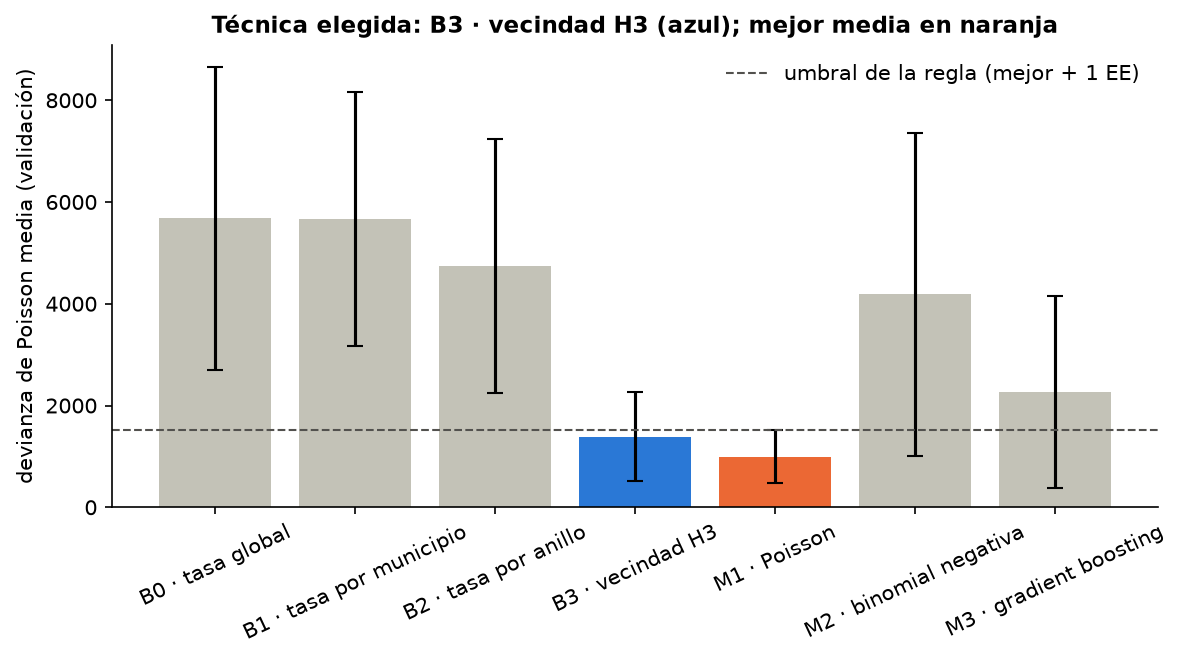
\includegraphics[width=0.72\textwidth]{imagenes/07_desarrollo/7_4_modelado/comparacion_tecnicas.png}
  \fuente{Elaboración propia, a partir de \var{04_modelado} (sección 6). Barras de error:
  $\pm 1$ error estándar; línea discontinua: umbral de la regla (mejor media más un error
  estándar); azul: técnica elegida; naranja: menor devianza media.}
\end{figure}

La tabla y la figura~\ref{fig:comparacion-tecnicas} permiten cinco lecturas:
\begin{enumerate}
  \item \textbf{Las líneas base por grupo apenas mejoran a la tasa global.} B1 y B2 tienen
        devianzas similares a B0, y su $D^2$ medio es negativo. En promedio predicen peor
        que la media del propio pliegue: una tasa común a todo un municipio o anillo no
        distingue entre zonas vecinas con comportamientos muy distintos.
  \item \textbf{La vecindad produce el mayor salto de la escalera.} B3 reduce la devianza
        de 4.743 a 1.389 y lleva el $D^2$ a 0,73. La información local es mucho más útil
        que las agrupaciones administrativas o por distancia.
  \item \textbf{M1 obtiene la menor devianza media (994,6)}, con un $D^2$ igual al de B3.
        Sin embargo, su calibración es de 0,807: en conjunto subestima el total de
        consultas en torno a un 19~\%.
  \item \textbf{M2 y M3 no compensan su complejidad.} M2 ordena bien las zonas (Spearman de
        0,843), pero su calibración de 0,354 indica que estima apenas un tercio del volumen
        real. Al corregir la sobredispersión da menos peso a las zonas de conteo alto,
        precisamente donde está casi todo el volumen. M3 alcanza un buen $D^2$ medio, pero
        su devianza es muy inestable entre pliegues.
  \item \textbf{La variabilidad entre pliegues es alta.} Las desviaciones estándar son del
        mismo orden que las medias. La tabla~\ref{tab:cv-pliegues} muestra la causa.
\end{enumerate}

\begin{table}[H]
  \centering
  \caption{Devianza de Poisson por pliegue de validación}
  \label{tab:cv-pliegues}
  \interlineadoSimple
  \small
  \begin{tabular}{@{}lrrrrr@{}}
    \toprule
    \textbf{Técnica} & \textbf{Pliegue 0} & \textbf{Pliegue 1} & \textbf{Pliegue 2} & \textbf{Pliegue 3} & \textbf{Pliegue 4} \\
    \midrule
    B0 & 2.811,7 & 3.914,3 & 17.477,0 & 2.510,8 & 1.666,5 \\
    B1 & 2.100,2 & 7.009,3 & 14.898,9 & 2.319,5 & 1.998,9 \\
    B2 & 2.274,0 & 2.886,6 & 14.697,3 & 2.052,4 & 1.803,1 \\
    B3 & 155,7 & 1.491,2 & 4.722,5 & 128,3 & 448,7 \\
    M1 & 145,5 & 1.199,8 & 2.956,3 & 241,8 & 429,6 \\
    M2 & 322,1 & 3.376,8 & 16.663,5 & 271,0 & 316,9 \\
    M3 & 107,2 & 971,0 & 9.753,8 & 147,5 & 349,9 \\
    \bottomrule
  \end{tabular}
  \fuente{Elaboración propia, a partir de \var{resultados/04_modelado/cv_por_pliegue.csv}.}
\end{table}

El pliegue 2 contiene bloques del centro de la ciudad, con conteos de decenas de miles de
consultas por zona, y su devianza es varias veces mayor que la de los demás en todas las
técnicas. Es ahí donde M3 falla más (9.753,8), probablemente porque sus árboles no
extrapolan bien a zonas con valores de los predictores poco frecuentes en el
entrenamiento de ese pliegue. En los pliegues periféricos (0, 3 y 4), B3, M1 y M3 tienen
errores de magnitud parecida. Esta heterogeneidad es la razón por la que la selección no
puede basarse solo en la media: la diferencia entre dos técnicas debe juzgarse frente a
la incertidumbre de esa media.

\subsection{Regla de selección}
\label{sec:regla-seleccion}

La técnica final se elige con una regla escrita en el protocolo antes de ejecutar ningún
modelo, conocida como \textbf{regla de un error estándar}: \emph{se elige la técnica más
simple de la escalera cuya devianza media no supere la mejor devianza media más un error
estándar de esta.}

El \emph{error estándar} (EE) mide cuánto podría variar la devianza media si los pliegues
fueran otros. Se calcula como la desviación estándar entre pliegues dividida por la raíz
del número de pliegues: $\text{EE} = \text{DE} / \sqrt{5}$. Dos técnicas cuyas medias
difieren menos de un EE no pueden distinguirse con los datos disponibles. En ese caso, la
regla prefiere la más simple, porque tiene menos supuestos, es más fácil de explicar y es
menos propensa al sobreajuste. La tabla~\ref{tab:regla-seleccion} aplica la regla.

\begin{table}[H]
  \centering
  \caption{Aplicación de la regla de un error estándar}
  \label{tab:regla-seleccion}
  \interlineadoSimple
  \small
  \begin{tabular}{@{}lrrcc@{}}
    \toprule
    \textbf{Técnica} & \textbf{\celda{Devianza\\media}} & \textbf{EE} & \textbf{\celda{$\leq$ umbral\\(1.518,8)}} & \textbf{Resultado} \\
    \midrule
    B0 & 5.676,1 & 2.972,1 & no & --- \\
    B1 & 5.665,3 & 2.494,1 & no & --- \\
    B2 & 4.742,7 & 2.495,1 & no & --- \\
    \textbf{B3} & \textbf{1.389,3} & \textbf{869,4} & \textbf{sí} & \textbf{elegida} \\
    M1 & 994,6 & 524,3 & sí & mejor media \\
    M2 & 4.190,1 & 3.174,7 & no & --- \\
    M3 & 2.265,9 & 1.878,3 & no & --- \\
    \bottomrule
  \end{tabular}
  \fuente{Elaboración propia, a partir de \var{resultados/04_modelado/regla_seleccion.csv}.
  Umbral $= 994{,}6 + 1{,}0 \times 524{,}3 = 1.518{,}8$.}
\end{table}

La mejor devianza media es la de M1 (994,6), con un error estándar de 524,3, lo que fija el
umbral en 1.518,8. Solo dos técnicas quedan por debajo: M1 y B3 (1.389,3). Como B3 ocupa
una posición anterior en la escalera, la regla \textbf{elige B3, el suavizado por vecindad
H3}.

La elección no responde a que B3 haya sido la primera técnica ejecutada ni a que tenga el
menor error. Las siete técnicas se evaluaron en las mismas condiciones y M1 obtuvo una
media menor. Se elige B3 porque la regla declarada de antemano establece que una diferencia
de 395 unidades de devianza, inferior a un error estándar, no justifica un modelo
paramétrico con supuestos que los propios datos contradicen, como la varianza igual a la
media. Hay además dos indicios, que no forman parte de la regla, a favor de B3 en el uso
previsto:
\begin{itemize}
  \item su calibración fuera de pliegue es de 0,977, frente a 0,807 de M1, de modo que
        reproduce mejor el volumen total;
  \item ordena las zonas algo mejor: calculado sobre todas las predicciones fuera de pliegue
        juntas, el Spearman es de 0,802 frente a 0,760. Estas cifras difieren de las de la
        tabla~\ref{tab:cv-resumen} (0,799 y 0,772), que son la media de los cinco valores
        calculados pliegue a pliegue.
\end{itemize}

La figura~\ref{fig:calibracion-oof} compara las predicciones fuera de pliegue de ambas
técnicas con lo observado.

\begin{figure}[H]
  \centering
  \caption{Observado frente a esperado fuera de pliegue: B3 y M1}
  \label{fig:calibracion-oof}
  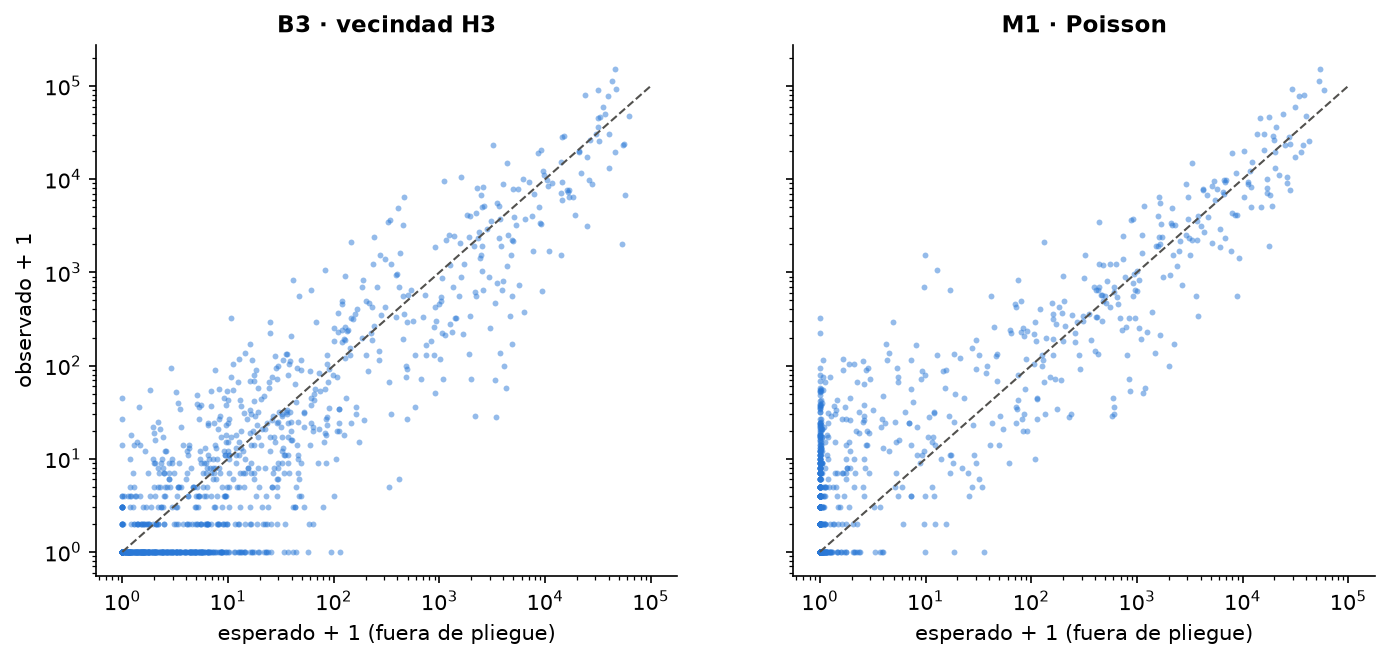
\includegraphics[width=0.9\textwidth]{imagenes/07_desarrollo/7_4_modelado/calibracion_oof.png}
  \fuente{Elaboración propia, a partir de \var{04_modelado} (sección 6). Ambos ejes en
  escala logarítmica (valor $+1$); la diagonal marca la coincidencia exacta.}
\end{figure}

Las dos nubes siguen la diagonal en los conteos altos, pero difieren en los bajos. B3
asigna a las zonas sin consultas esperados pequeños y variados, tomados de sus vecinas. M1
acumula muchas zonas con esperado cercano a cero, que en la columna izquierda aparecen con
conteos observados de hasta cientos de consultas. Esa diferencia es relevante para el
problema: una técnica que asigna esperado casi nulo a una zona no puede detectar en ella
una brecha negativa.

La técnica elegida tiene también un límite: B3 aprende de los vecinos, así que las zonas
que conviven con un polo de actividad heredan una tasa muy alta. Sus consecuencias se
examinan en la evaluación.

% ============================================================
%  7.5. EVALUACIÓN Y RESULTADOS  -- parte del capítulo 7
%  ------------------------------------------------------------
%  Archivo separado para que cada fase de CRISP-DM se pueda
%  editar y compilar por separado. Solo contenido: el formato,
%  los rótulos y las referencias los resuelve el preámbulo.
%  Los \label originales se conservan sin cambios.
% ============================================================
\section{Evaluación y Resultados}
\label{sec:evaluacion-resultados}

Esta sección documenta la quinta fase de CRISP-DM, ejecutada mediante cinco scripts
(\var{21_hypothesis_tests.py} a \var{28_ranking_explainer.py}) sobre las
predicciones de los cuatro modelos de la sección~\ref{sec:modelado}.

\subsection{Métricas y resultados por modelo}
\label{sec:resultados-modelo}

Se reportan tres métricas, cada una con un rol distinto dado que el objetivo es fuertemente
asimétrico (sección~\ref{sec:seleccion-algoritmos}): el \textbf{MAE} (error absoluto medio),
interpretable directamente en consultas por semana; el \textbf{RMSE}, que penaliza más los
errores grandes y es por tanto sensible a la presencia de valores extremos; y el
\textbf{R\textsuperscript{2}}, la proporción de varianza explicada respecto de predecir
siempre la media.

\begin{table}[htbp]
  \centering
  \caption{Desempeño comparado en el conjunto de prueba (8 semanas nunca vistas)}
  \label{tab:resultados-modelos}
  \interlineadoSimple
  \begin{tabular}{lrrr}
    \toprule
    \textbf{Modelo} & \textbf{MAE} & \textbf{RMSE} & \textbf{R\textsuperscript{2}} \\
    \midrule
    \textbf{Random Forest (final)} & \textbf{10,19} & \textbf{80,70} & \textbf{0,656} \\
    Base estacional (media móvil 4 sem.) & 11,05 & 85,70 & 0,613 \\
    Base ingenua (persistencia, $t-1$) & 11,30 & 91,90 & 0,555 \\
    XGBoost & 13,85 & 102,82 & 0,442 \\
    Lasso & 44,03 & 520,76 & $-13,305$ \\
    Ridge & 48,97 & 559,13 & $-15,491$ \\
    \bottomrule
  \end{tabular}
  \fuente{Elaboración propia, a partir de \var{19_model_comparison.py} ---
  \var{reports/03_modeling/02_model_comparison.md}.}
\end{table}

\begin{figure}[htbp]
  \centering
  \caption{Predicho vs. observado, Random Forest, conjunto de prueba}
  \label{fig:pred-vs-obs}
  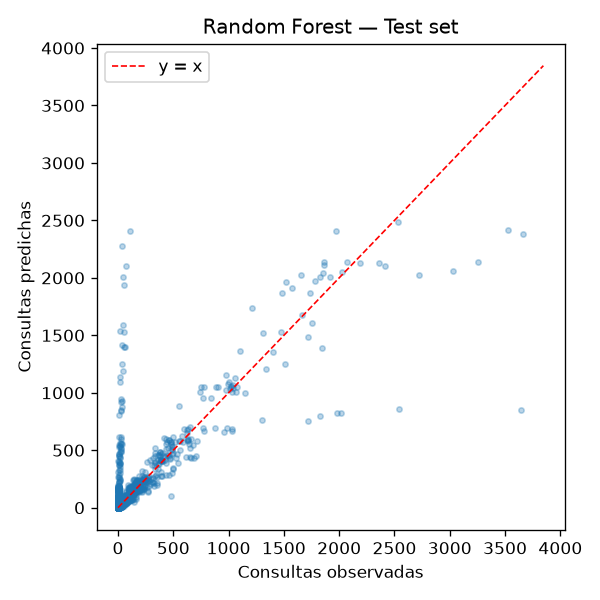
\includegraphics[width=0.7\textwidth]{imagenes/fig_pred_vs_obs_rf.png}
  \fuente{Elaboración propia, a partir de \var{19_model_comparison.py}.}
\end{figure}

\subsubsection{Hallazgo: inestabilidad de extrapolación de los modelos lineales}

Ridge y Lasso muestran R\textsuperscript{2} fuertemente negativo en prueba pese a un ajuste
razonable en entrenamiento (MAE de 30,06 y 25,57 respectivamente): 50 y 42 de las 12.416
predicciones de cada uno alcanzan el techo de seguridad de extrapolación impuesto sobre la
reversión \texttt{expm1} (sección~\ref{sec:tipo-problema}). La causa es la combinación de una
tendencia sostenida --\var{week_idx} toma en prueba valores nunca vistos en
entrenamiento-- con la asimetría extrema del objetivo (Gini~$=0{,}934$,
sección~\ref{sec:sensibilidad-h3}): un pequeño error en escala logarítmica se amplifica
exponencialmente al revertir la transformación. \textbf{No es un defecto de implementación:
es evidencia de que la relación entre demanda y condiciones territoriales no es lineal.} Los
modelos de árboles no sufren este problema porque sus predicciones están acotadas por los
valores observados en las hojas de entrenamiento.

\subsection{Sobreajuste y subajuste}
\label{sec:sobreajuste}

\begin{table}[htbp]
  \centering
  \caption{Brecha entre entrenamiento y prueba (MAE)}
  \label{tab:brecha-train-test}
  \interlineadoSimple
  \begin{tabular}{lrrr}
    \toprule
    \textbf{Modelo} & \textbf{MAE entrenamiento} & \textbf{MAE prueba} & \textbf{Brecha} \\
    \midrule
    Random Forest & 2,19 & 10,19 & $+8,00$ \\
    XGBoost & 2,09 & 13,85 & $+11,76$ \\
    Lasso & 25,57 & 44,03 & $+18,46$ \\
    Ridge & 30,06 & 48,97 & $+18,92$ \\
    \bottomrule
  \end{tabular}
  \fuente{Elaboración propia, a partir de \var{19_model_comparison.py}.}
\end{table}

La brecha de Random Forest ($+8{,}00$) es menor que la de XGBoost ($+11{,}76$) pese a
hiperparámetros de complejidad similar, señal de menor sobreajuste relativo. Las curvas de
aprendizaje --Random Forest reentrenado con tamaños de entrenamiento crecientes, evaluado
contra una ventana de validación de 13 semanas no vista-- refuerzan esta lectura.

\begin{figure}[htbp]
  \centering
  \caption{Curva de aprendizaje de Random Forest}
  \label{fig:curva-aprendizaje}
  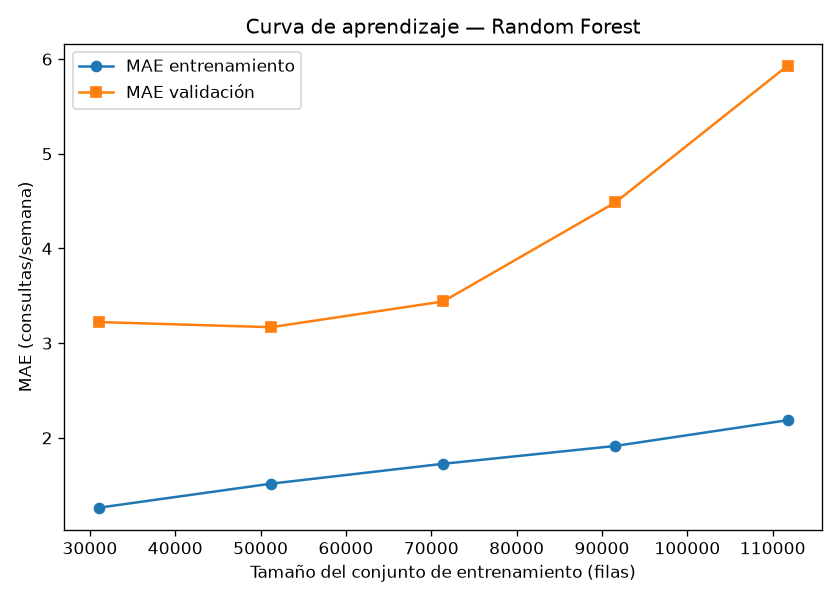
\includegraphics[width=0.7\textwidth]{imagenes/fig_learning_curve.png}
  \fuente{Elaboración propia, a partir de \var{23_error_analysis.py} ---
  \var{reports/04_evaluation/03_error_analysis.md}.}
\end{figure}

La brecha entrenamiento-validación crece de forma moderada a medida que aumenta el tamaño de
entrenamiento ($+1{,}96 \to +1{,}65 \to +1{,}71 \to +2{,}57 \to +3{,}74$), con un MAE de
entrenamiento que se mantiene bajo (1,26 a 2,19) mientras el de validación oscila en un rango
razonable (3,2 a 5,9): la firma esperada de un árbol de profundidad acotada
(\var{max_depth}$=10$) que ajusta ruido de forma limitada, sin señal de varianza
descontrolada. La curva tiene solo cinco puntos por costo computacional --cada uno reentrena
un modelo completo--, suficiente para descartar sobreajuste severo pero no para un
diagnóstico fino.

\subsection{Contraste de hipótesis}
\label{sec:contraste-hipotesis}

\subsubsection{H1 --- Brecha de cobertura centro-periferia}

Se contrasta si las celdas periféricas (mayor distancia al centro) tienen una tasa de
demanda no resuelta (\var{pct_uncovered_orig}) significativamente mayor que las
centrales. La unidad de análisis es la \textbf{celda}, no la celda-semana: se promedia
\var{pct_uncovered_orig} sobre todas las semanas de cada celda, porque tratar cada
semana como observación independiente constituiría pseudorreplicación --inflaría el tamaño
muestral de 1.552 a decenas de miles y produciría un valor p espuriamente pequeño. Los
grupos se definen por la mediana de \var{dist_center_km} (15,49~km): 776 celdas
centrales y 776 periféricas, un corte simple y documentado pero arbitrario, que no
corresponde a ningún límite administrativo real.

\begin{table}[htbp]
  \centering
  \caption{Contraste H1: tasa de demanda no resuelta por grupo territorial}
  \label{tab:h1-resultado}
  \interlineadoSimple
  \begin{tabular}{lrr}
    \toprule
    \textbf{Grupo} & \textbf{n celdas} & \textbf{Media \var{pct_uncovered_orig}} \\
    \midrule
    Central & 776 & 0,213 \\
    Periferia & 776 & 0,351 \\
    \bottomrule
  \end{tabular}
  \fuente{Elaboración propia, a partir de \var{21_hypothesis_tests.py} ---
  \var{reports/04_evaluation/01_hypothesis_tests.md}.}
\end{table}

La prueba de Shapiro-Wilk rechazó la normalidad en ambos grupos ($p=2{,}18\times10^{-41}$ en
el centro, $p=1{,}423\times10^{-38}$ en la periferia) --resultado esperable, dado que la
variable es una proporción con masa concentrada en 0 y 1--, lo que fundamenta el uso de la
prueba U de Mann-Whitney, no paramétrica. El resultado es concluyente: estadístico
$341{.}618{,}0$, $p=6{,}101\times10^{-9}$, significativo a $\alpha=0{,}05$, con una
correlación biserial por rangos de $-0{,}135$ (tamaño de efecto pequeño, dado el tamaño
muestral). \textbf{Se confirma H1}: las celdas periféricas tienen una tasa de demanda no
resuelta significativamente mayor que las centrales.

\subsubsection{H2 --- Random Forest frente a la línea base estacional}

Se contrasta si el error del modelo final es significativamente menor que el de la media
móvil de 4 semanas. El test de Diebold-Mariano, diseñado específicamente para comparar
exactitud predictiva entre dos modelos sobre una serie temporal, opera sobre la serie
semanal de 8 puntos de prueba: con esa potencia insuficiente por construcción, el resultado
no es significativo (estadístico $-0{,}705$, $p=0{,}503$). Un resultado no significativo no
implica equivalencia entre los modelos, solo que ocho semanas no alcanzan para distinguirlos
con confianza; la ventana de prueba se fijó en la sección~\ref{sec:particion-cronologica}
para preservar datos de entrenamiento, no para maximizar la potencia de este contraste.

Se complementa con una prueba de Wilcoxon de rangos con signo, pareada por celda (1.552
observaciones, potencia suficiente): estadístico $287.045{,}0$, $p=0{,}0326$, significativo.
A primera vista esto contradice que Random Forest solo supere a la base en el 31,0~\% de las
celdas; la explicación está en la magnitud, no en el conteo:

\begin{table}[htbp]
  \centering
  \caption{Dónde gana cada método (test de Wilcoxon pareado por celda)}
  \label{tab:h2-desglose}
  \interlineadoSimple
  \begin{tabularx}{\textwidth}{@{}Xrrr@{}}
    \toprule
    \textbf{Grupo} & \textbf{n celdas} & \textbf{Dif. media (RF $-$ base)} & \textbf{Demanda media} \\
    \midrule
    Gana Random Forest & 481 & $-3,72$ & 42,9 consultas/sem. \\
    Gana la base estacional & 632 & $+0,71$ & 13,8 consultas/sem. \\
    Empate exacto & 439 & --- & --- \\
    \bottomrule
  \end{tabularx}
  \fuente{Elaboración propia, a partir de \var{21_hypothesis_tests.py}.}
\end{table}

Random Forest gana por un margen grande en celdas de alta demanda y pierde por un margen
pequeño en celdas casi sin actividad. \textbf{Se confirma H2, con matices}: la ventaja de
Random Forest sobre la línea base es estadísticamente significativa y está concentrada
exactamente en las celdas de mayor demanda --el segmento operativamente más relevante--, no
distribuida de manera uniforme. Reportar solo el valor p o solo el porcentaje de celdas
ganadas habría sido engañoso en direcciones opuestas.

\subsection{Análisis de errores}
\label{sec:analisis-errores}

La media de residuos de Random Forest en prueba es $-4{,}758$. Esta cifra no debe calificarse
de sesgo despreciable: representa cerca de la mitad del MAE de prueba (10,19), lo que indica
una tendencia sistemática a la sobrepredicción, atribuible en buena parte a las semanas
parciales que se describen a continuación.

\begin{figure}[htbp]
  \centering
  \caption{Distribución de residuos por celda, conjunto de prueba}
  \label{fig:residuos}
  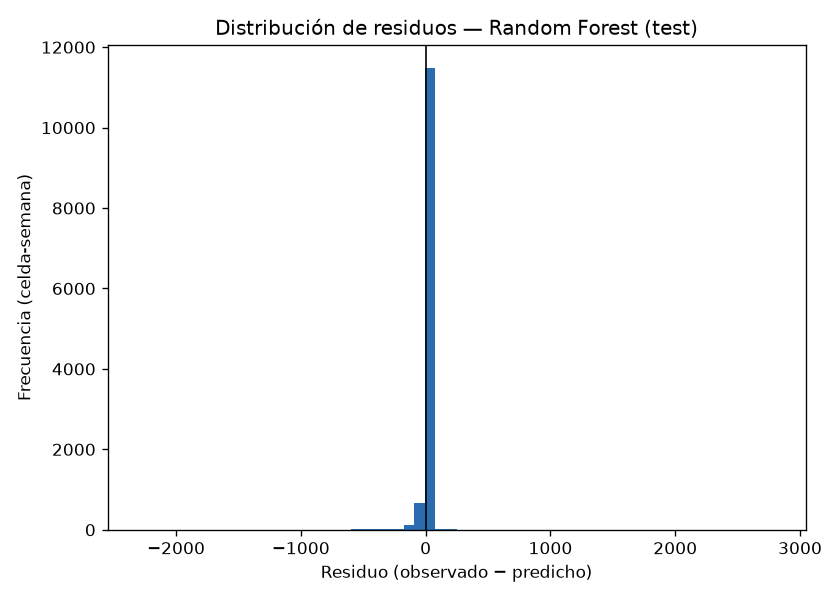
\includegraphics[width=0.65\textwidth]{imagenes/fig_residuals_by_cell.png}
  \fuente{Elaboración propia, a partir de \var{23_error_analysis.py}.}
\end{figure}

\subsubsection{Hallazgo: dos semanas de prueba son fragmentos de un día}
\label{sec:semanas-parciales}

Al construir la serie semanal agregada se detectó que la demanda observada total cae a
apenas 1--3~\% de una semana normal en dos de las ocho semanas de prueba: 2024-W18 (909
consultas, la semana de reanudación tras el vacío, con solo unas 5 horas de datos) y
2024-W23 (1.367 consultas, el corte final del dataset, con solo unas 11 horas de datos). No
se trata de semanas con demanda real más baja sino de fragmentos de un solo día --un
artefacto de cobertura de exportación no advertido al fijar la partición
(sección~\ref{sec:particion-cronologica}).

\begin{table}[htbp]
  \centering
  \caption{Impacto de las semanas parciales sobre las métricas del modelo final}
  \label{tab:semanas-parciales}
  \interlineadoSimple
  \begin{tabular}{lrrr}
    \toprule
    \textbf{Escenario} & \textbf{MAE} & \textbf{RMSE} & \textbf{R\textsuperscript{2}} \\
    \midrule
    Las 8 semanas de prueba (resultado principal) & 10,19 & 80,70 & 0,656 \\
    Las 6 semanas completas (sin las parciales) & 5,91 & 52,87 & 0,889 \\
    \bottomrule
  \end{tabular}
  \fuente{Elaboración propia, a partir de \var{23_error_analysis.py} ---
  \var{reports/04_evaluation/03_error_analysis.md}.}
\end{table}

Esta monografía reporta \textbf{ambas cifras juntas}, y no una sola. El MAE de 10,19 se
mantiene como resultado principal por ser la evaluación más conservadora y no requerir una
decisión de exclusión posterior a la observación de los datos; el MAE de 5,91 es la
estimación más representativa del desempeño en una semana calendario completa, y es
consistente con el historial de validación cruzada (2,8 a 6,2,
sección~\ref{sec:hiperparametros}), frente al cual 10,19 resulta atípico una vez comprendida
su causa. Presentar solo la segunda cifra sería selección posterior favorable; presentar solo
la primera ocultaría que el error está inflado por un artefacto identificado y rastreado
hasta el dato crudo.

\begin{figure}[htbp]
  \centering
  \caption{Estabilidad temporal del error semanal en el conjunto de prueba}
  \label{fig:estabilidad-error}
  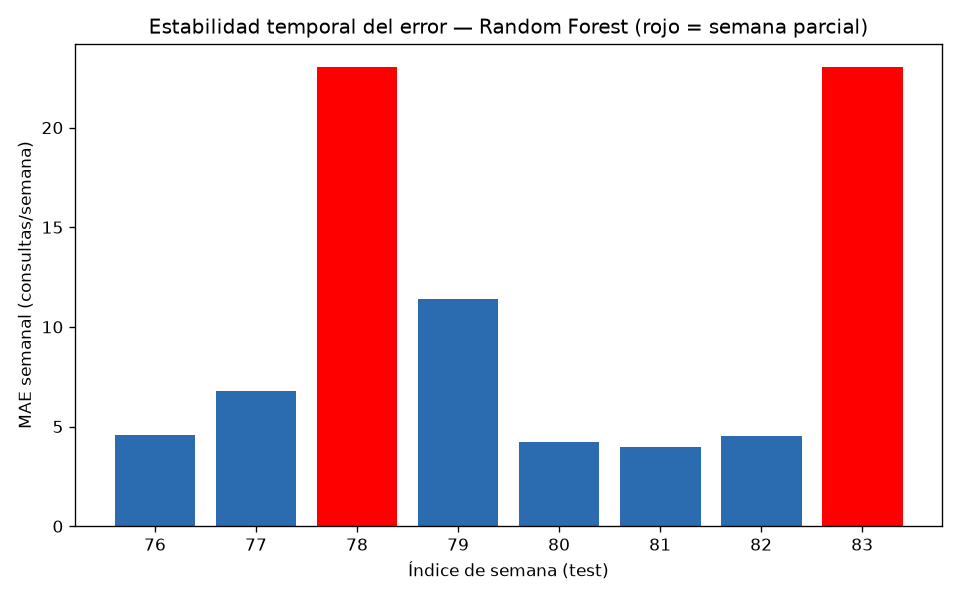
\includegraphics[width=0.7\textwidth]{imagenes/fig_weekly_error_stability.png}
  \fuente{Elaboración propia, a partir de \var{23_error_analysis.py}. Las semanas
  2024-W18 y 2024-W23 (parciales) se resaltan.}
\end{figure}

El artefacto no se limita a las dos semanas donde se originó: 2024-W19, la semana
inmediatamente posterior a 2024-W18, también registra un MAE elevado (11,38, más del doble de
la mediana de las semanas limpias) pese a no tener ningún problema de datos propio, porque
hereda de 2024-W18 un \var{lag1_n_queries_orig} artificialmente bajo (909 consultas en
vez de un nivel normal de más de 40.000). El horizonte de pronóstico evaluado no muestra
degradación progresiva por sí solo; la única inestabilidad detectada tiene una causa puntual
e identificada, no un problema estructural del modelo.

\subsection{Interpretación desde el problema original}
\label{sec:interpretacion-resultados}

La pregunta de investigación --cómo se distribuye la demanda de información de transporte no
resuelta y qué características del territorio se asocian con esa distribución-- se responde
con evidencia convergente de tres análisis. Primero, H1 confirma estadísticamente que la
brecha de cobertura es mayor en la periferia. Segundo, el gradiente espacial de demanda es
real: la correlación de Spearman entre \var{dist_center_km} y la demanda decae tanto
para la demanda observada ($\rho=-0{,}615$, $p=2{,}8\times10^{-162}$) como para la predicha
($\rho=-0{,}618$, $p=3{,}3\times10^{-164}$).

\begin{figure}[htbp]
  \centering
  \caption{Demanda semanal observada vs. distancia al centro}
  \label{fig:demanda-distancia}
  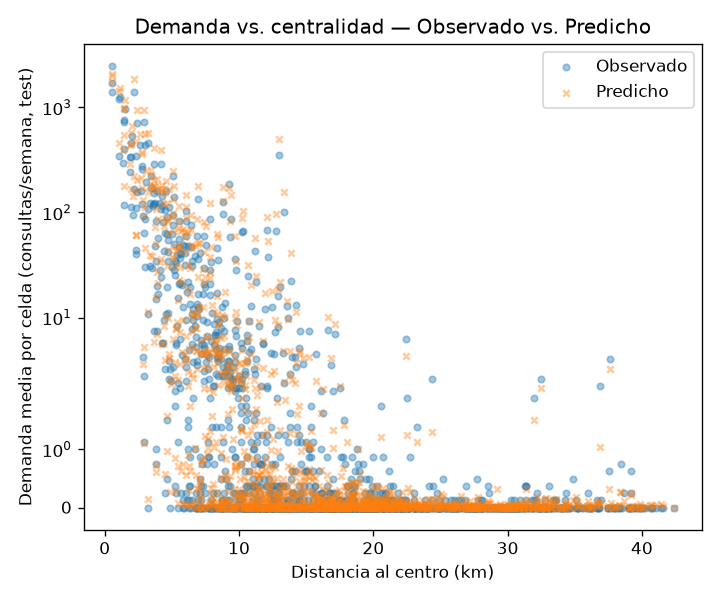
\includegraphics[width=0.7\textwidth]{imagenes/fig_demand_vs_distance.png}
  \fuente{Elaboración propia, a partir de \var{22_results_analysis.py} ---
  \var{reports/04_evaluation/02_results_analysis.md}.}
\end{figure}

Tercero, H2 muestra que el valor predictivo del modelo está concentrado exactamente donde
más importa operativamente: las celdas de mayor demanda. En conjunto, la periferia combina
\textbf{menor demanda absoluta} con \textbf{peor cobertura relativa} --un patrón consistente
con zonas de expansión urbana con transporte formal insuficiente, y no con una simple falta
de interés de los usuarios; debe recordarse, como se ha señalado en capítulos anteriores, que
``demanda'' significa aquí consultas de planificación --intención de viaje-- y no
desplazamientos confirmados.

\begin{figure}[htbp]
  \centering
  \caption{Demanda semanal agregada, observada vs. predicha (conjunto de prueba)}
  \label{fig:demanda-semanal}
  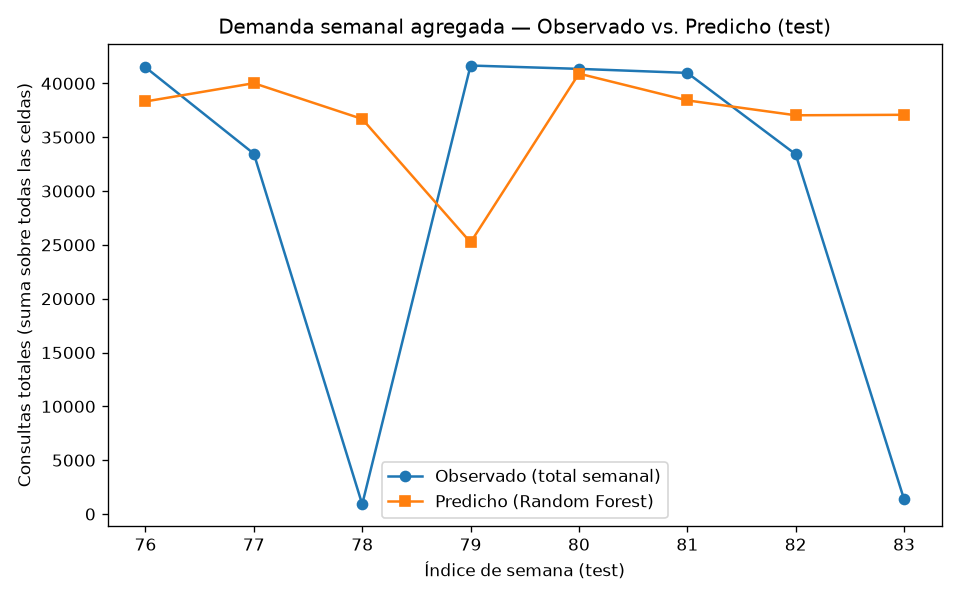
\includegraphics[width=0.7\textwidth]{imagenes/fig_weekly_demand_test.png}
  \fuente{Elaboración propia, a partir de \var{22_results_analysis.py}. Las semanas
  2024-W18 y 2024-W23 (parciales, sección~\ref{sec:semanas-parciales}) explican los mayores
  desvíos agregados de la serie.}
\end{figure}

\subsubsection{Importancia de variables}
\label{sec:importancia-variables}

Las variables autorregresivas dominan la importancia en Random Forest y XGBoost
(\var{roll_mean4_n_queries_orig} explica el 97,9~\% de la reducción de impureza en
Random Forest), coherente con la fuerte autocorrelación semanal de la demanda documentada en
la sección~\ref{sec:cobertura-temporal}.

\begin{figure}[htbp]
  \centering
  \caption{Importancia de variables (Gini), Random Forest}
  \label{fig:importancia-rf}
  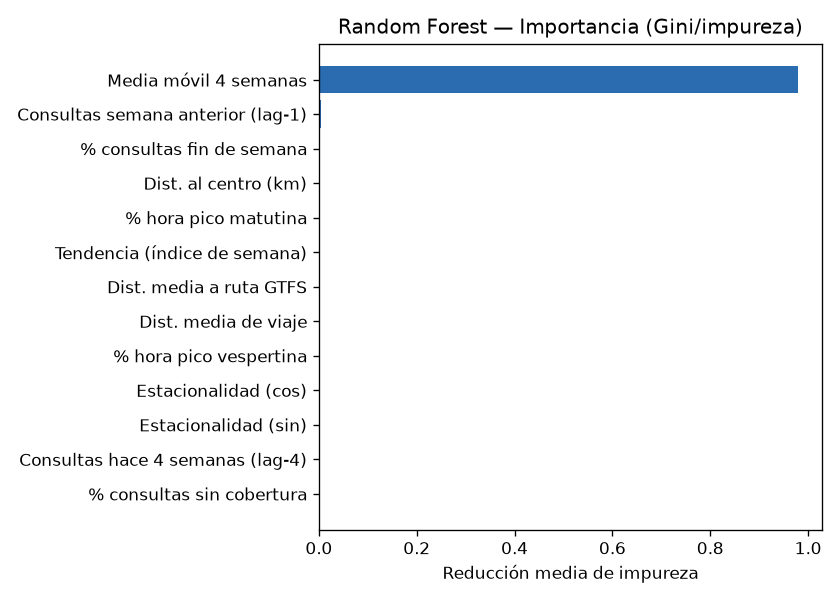
\includegraphics[width=0.65\textwidth]{imagenes/fig_feature_importance_rf.png}
  \fuente{Elaboración propia, a partir de \var{20_feature_importance.py} ---
  \var{reports/03_modeling/03_feature_importance.md}.}
\end{figure}

La señal territorial es más relevante de lo que sugiere la importancia por ganancia: en
XGBoost, \var{dist_center_km} ocupa la octava posición por ganancia pero asciende al
tercer lugar por magnitud media de SHAP, un método de interpretabilidad que atribuye a cada
variable su contribución marginal a cada predicción individual. Lasso --que lleva 9 de 13
coeficientes a cero, actuando como selector de variables-- conserva precisamente
\var{dist_center_km} (coeficiente estandarizado $-0{,}424$),
\var{roll_mean4_n_queries_orig} ($+0{,}396$), \var{lag1_n_queries_orig}
($+0{,}187$) y \var{pct_uncovered_orig} ($-0{,}077$) como la señal independiente más
robusta, con signos coherentes con H1: mayor distancia al centro y mayor proporción sin
cobertura se asocian con menor demanda.

\subsection{¿Sirve el modelo para priorizar? Un criterio preinscrito, refutado}
\label{sec:sirve-para-priorizar}

Si el modelo no gana por precisión de valor de forma contundente, el argumento operativo que
quedaba era que, aunque no acertara la magnitud exacta, ordenara bien las celdas para efectos
de priorización territorial. Esta sección lo somete a prueba con un criterio \textbf{declarado
antes de observar los resultados}: el modelo sirve para priorizar si ordena mejor que la
media móvil de 4 semanas, con diferencia media positiva, signo consistente entre semanas y
una prueba pareada que no lo contradiga. Declarar el criterio de antemano es lo que distingue
un hallazgo de una racionalización posterior, precisamente porque la comparación podía salir
en contra.

\textbf{El criterio no se cumple.} Promediando sobre las 6 semanas completas de prueba (se
excluyen las semanas parciales de la sección~\ref{sec:semanas-parciales}):

\begin{table}[htbp]
  \centering
  \caption{Métricas de ordenamiento territorial, promedio de las 6 semanas completas de prueba}
  \label{tab:ranking-metricas}
  \interlineadoSimple
  \begin{tabular}{lrrr}
    \toprule
    \textbf{Método} & \textbf{vRecall@20} & \textbf{NDCG@20} & \textbf{$\tau$-b de Kendall} \\
    \midrule
    \textbf{Base: media móvil 4 sem.} & \textbf{0,996} & \textbf{0,999} & \textbf{0,853} \\
    Random Forest & 0,995 & 0,996 & 0,850 \\
    XGBoost & 0,993 & 0,997 & 0,843 \\
    Base: persistencia ($t-1$) & 0,983 & 0,994 & 0,800 \\
    Ranking aleatorio (piso) & 0,022 & 0,104 & 0,001 \\
    \bottomrule
  \end{tabular}
  \fuente{Elaboración propia, a partir de \var{26_ranking_metrics.py} ---
  \var{reports/04_evaluation/04_ranking_metrics.md}.}
\end{table}

Random Forest no supera a la media móvil de 4 semanas en ninguna de las 6 semanas completas,
en ninguna de las métricas de ordenamiento evaluadas: el recuento de volumen alcanzable en
las 20 celdas elegidas (vRecall@20, la métrica principal, continua e insensible a empates), la
calidad del orden ponderada por posición (NDCG@20, calculada sobre relevancia logarítmica
porque con conteos crudos todos los métodos saturan por encima de 0,97) y la correlación de
rangos ($\tau$-b de Kendall, restringida a las celdas con demanda media de entrenamiento
$\geq 5$ para no dejar que domine el 76,6~\% de observaciones con demanda nula en prueba).
Ningún corte rescata la comparación: ni el estrato de demanda media (correlación de Spearman
0,957 contra 0,958 de la base) ni el ranking de los cambios semana a semana (0,458 contra
0,514, también a favor de la base).

\begin{figure}[htbp]
  \centering
  \caption{Comparación de métricas de ordenamiento por método y semana}
  \label{fig:ranking-comparacion}
  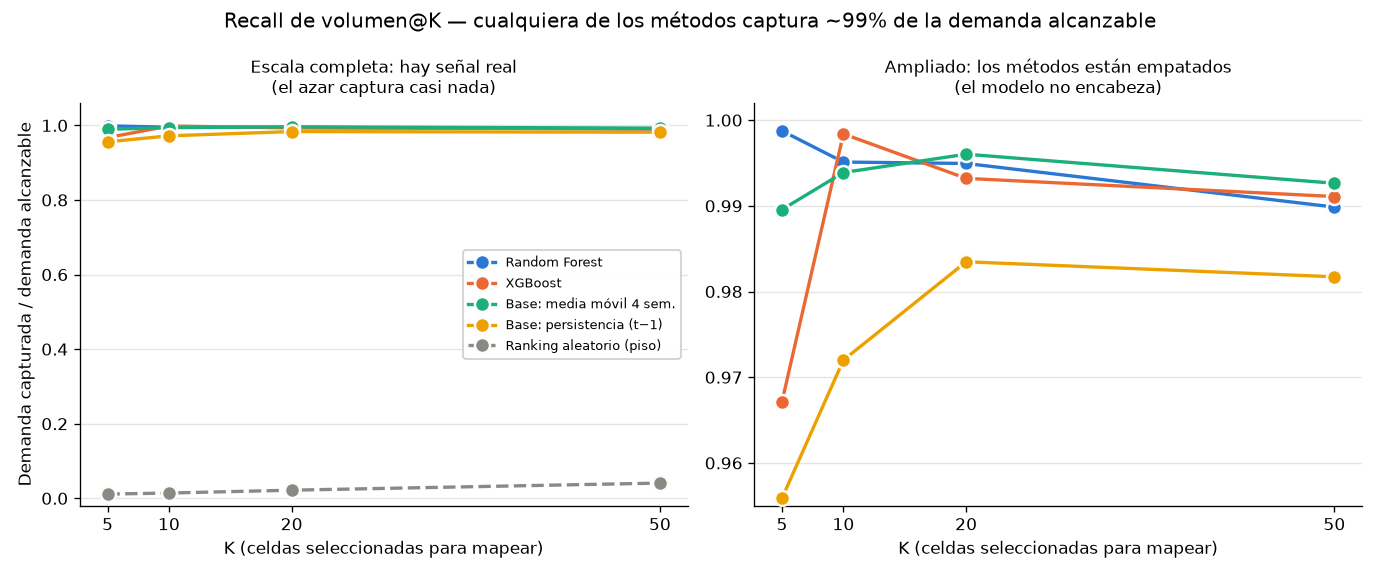
\includegraphics[width=0.75\textwidth]{imagenes/fig_ranking_comparison.png}
  \fuente{Elaboración propia, a partir de \var{26_ranking_metrics.py}.}
\end{figure}

\begin{figure}[htbp]
  \centering
  \caption{Cómo se calcula e interpreta la métrica de priorización}
  \label{fig:ranking-explicador}
  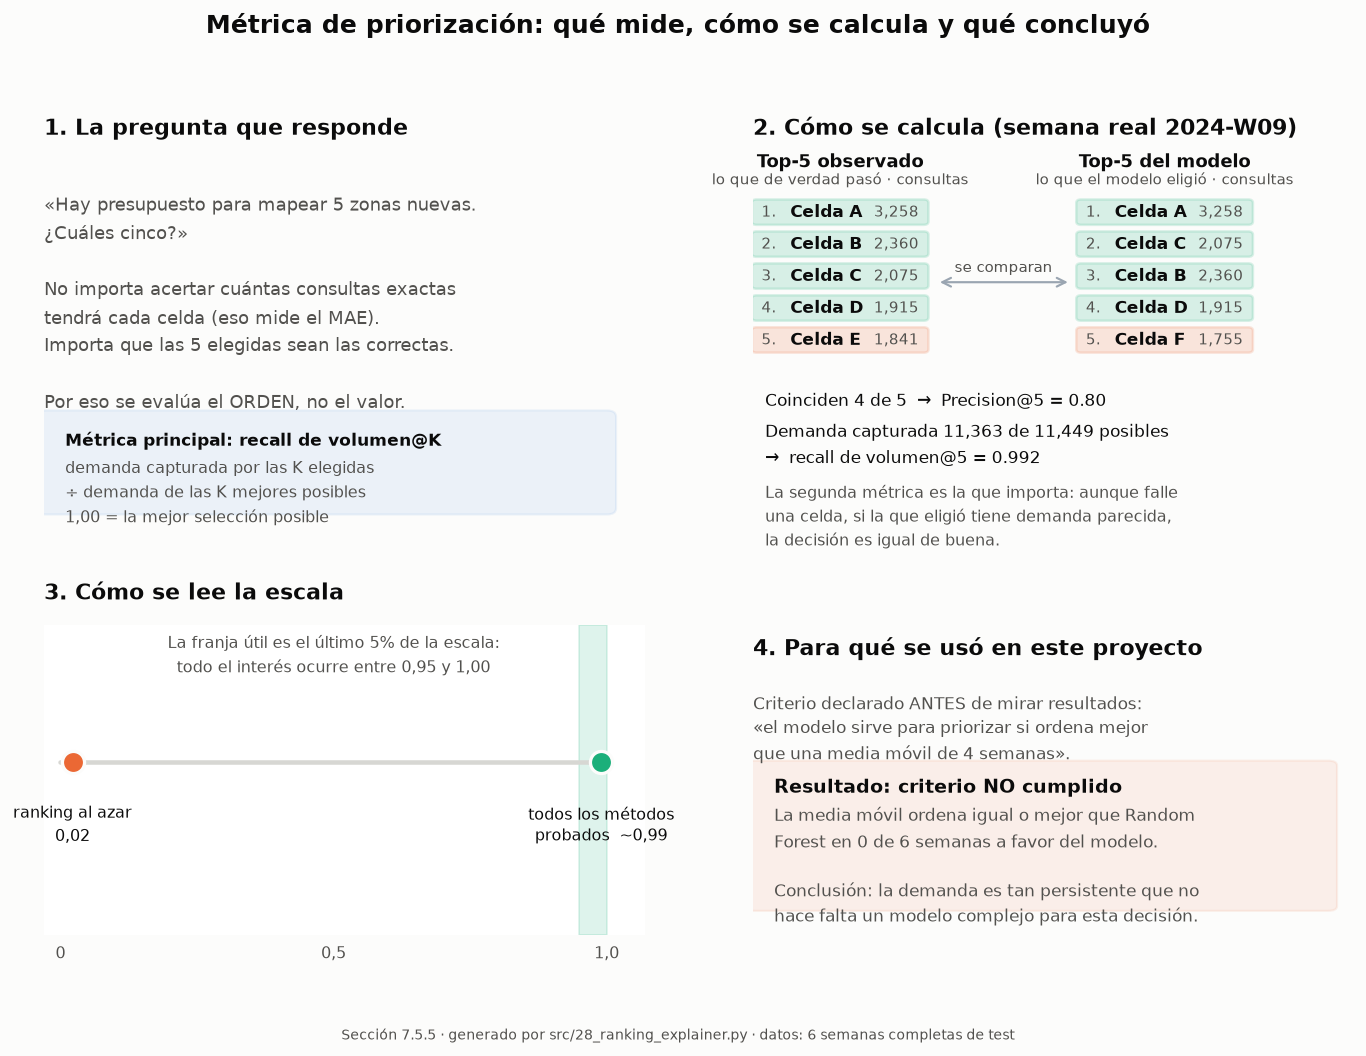
\includegraphics[width=0.75\textwidth]{imagenes/fig_ranking_explainer.png}
  \fuente{Elaboración propia, a partir de \var{28_ranking_explainer.py}.}
\end{figure}

Un coeficiente de correlación de rangos alto --como el $\rho=0{,}877$ entre demanda
observada y predicha reportado en la sección~\ref{sec:interpretacion-resultados}-- es fácil
de obtener cuando la distribución subyacente está tan concentrada como aquí (Gini$=0{,}934$,
sección~\ref{sec:sensibilidad-h3}): el ordenamiento de celdas es casi invariante entre
semanas, de modo que cualquier estimador --incluida una media móvil, e incluso la
persistencia-- reproduce ese orden. Esa cifra mide que el modelo no destruye una señal
trivialmente disponible; no mide que aporte capacidad de ordenamiento propia, que es
justamente lo que esta comparación contra competencia refuta.

\textbf{Este resultado no debilita el trabajo, lo fortalece.} Se obtuvo con un criterio
declarado de antemano y una comparación que podía salir en contra, exactamente lo que
distingue un hallazgo de una racionalización posterior. La formulación correcta es que, para
decidir qué celdas mapear a un horizonte de una semana, no se justifica un modelo complejo:
una media móvil de cuatro semanas ordena igual o mejor, y es además transparente, barata de
operar y auditable. La contribución de este trabajo está en el pipeline reproducible, la
caracterización territorial y el diagnóstico de cobertura (H1), no en la superioridad de un
estimador de valor. El alcance de esta refutación es específico: vale para horizonte de una
semana; a horizontes mayores la media móvil envejece y el modelo podría mostrar ventaja, pero
esa prueba no se realizó --requeriría reconstruir los rezagos y reentrenar-- y queda
declarada como pendiente, no como ventaja supuesta.

\subsection{Selección y justificación del modelo final}
\label{sec:seleccion-final}

\textbf{Random Forest se selecciona como modelo final}, con un criterio explícito aplicado
en el siguiente orden: menor MAE de prueba entre los cuatro modelos ajustados (10,19); menor
brecha entre entrenamiento y prueba que XGBoost ($+8{,}00$ frente a $+11{,}76$); y único
modelo que supera de forma consistente a ambas líneas base. XGBoost se descarta pese a un MAE
de validación cruzada competitivo (4,17 frente a 3,58 de Random Forest): en el conjunto de
prueba resulta peor (13,85) que la propia línea base estacional (11,05) --un caso concreto de
por qué no debe elegirse un modelo por su posición en una única métrica de validación. Haber
sido el primer modelo ejecutado no cuenta como criterio, exigencia explícita de la guía de la
materia.

La selección se sostiene también en interpretabilidad y costo computacional: Random Forest no
requiere las precauciones de extrapolación que exigirían Ridge o Lasso en producción, y su
tiempo de entrenamiento es compatible con la cadencia de reentrenamiento trimestral propuesta
en la sección~\ref{sec:despliegue}. Su ventaja frente a la línea base es real y
estadísticamente significativa donde más importa operativamente (H2), aunque --como se
estableció en la sección~\ref{sec:sirve-para-priorizar}-- esa ventaja no se traduce en una
mejor capacidad de ordenamiento territorial que una media móvil simple.

% ============================================================
%  7.6. DESPLIEGUE  -- parte del capítulo 7
%  ------------------------------------------------------------
%  Archivo separado para que cada fase de CRISP-DM se pueda
%  editar y compilar por separado. Solo contenido: el formato,
%  los rótulos y las referencias los resuelve el preámbulo.
%  Los \label originales se conservan sin cambios.
% ============================================================
\section{Despliegue}
\label{sec:despliegue}

Esta sección documenta la sexta fase de CRISP-DM, construida sobre el modelo final de la
sección~\ref{sec:seleccion-final} y la evaluación de la
sección~\ref{sec:evaluacion-resultados}.

\subsection{Caso de uso en un contexto real}

El resultado del proyecto es una \textbf{capa analítica de priorización territorial}: demanda
esperada de consultas por celda H3 y semana, cruzada con la brecha de cobertura GTFS. No
sustituye la decisión humana de planificación de rutas: implica error real por celda (MAE de
10,19, o 5,91 en semanas completas, sección~\ref{sec:semanas-parciales}), y H2
(sección~\ref{sec:contraste-hipotesis}) mostró que la ventaja del modelo se concentra en
celdas de alta demanda, no en todas. El uso concreto propuesto es priorizar, dentro del
proceso de mapeo voluntario de rutas de Trufi App descrito en la
sección~\ref{sec:comprension-negocio}, qué celdas de baja cobertura conviene atender primero.

\subsection{Prototipo y arquitectura}

Se construyó un \textbf{servicio real y ejecutable}, no solo un diagrama: \var{src/trufi_ds/api.py}
(FastAPI), que carga el modelo Random Forest final y reconstruye, para cualquier celda, el
vector de variables de la semana siguiente a la última observada, con exactamente la misma
lógica de ingeniería de características usada en el entrenamiento
(sección~\ref{sec:seleccion-algoritmos}). Expone \texttt{GET /predict?cell=...} para una
celda individual y \texttt{GET /cells/top?n=...} para el caso de uso de priorización. La guía
UMSS admite una propuesta fundamentada cuando no hay despliegue completo; un prototipo
verificable localmente satisface el requisito con evidencia y no solo con intención.

\begin{figure}[htbp]
  \centering
  \caption{Arquitectura de actualización y consumo del modelo}
  \label{fig:arquitectura}
  
\includegraphics[width=0.85\textwidth]{imagenes/logo_facultad.png}
  \fuente{Elaboración propia. Diagrama descrito textualmente a continuación; el flujo
  completo (Mermaid) está documentado en \var{reports/05_deployment/01_deployment_architecture.md}.}
\end{figure}

El flujo conecta componentes que ya existen como código en este repositorio, sin
componentes hipotéticos: el feed GTFS (actualización semanal, \var{run_update_pipeline.py})
y las exportaciones de consultas alimentan el cálculo de cobertura
(sección~\ref{sec:cobertura-gtfs}) y la tabla de indicadores
(sección~\ref{sec:tabla-indicadores}); de ahí se derivan, por un lado, el reentrenamiento
trimestral del modelo (\var{18_model_training.py}) y, por otro, la reconstrucción del
panel de features que consume el servicio de predicción; el plan de monitoreo
(sección~\ref{sec:monitoreo}) vigila el servicio en producción.

\subsection{Consumo del modelo}

Los siguientes son ejemplos reales, obtenidos ejecutando el servicio contra los datos y el
modelo actuales del repositorio --no respuestas hipotéticas--, incluido un caso de error
controlado.

\begin{table}[htbp]
  \centering
  \caption{Ejemplos de consumo del prototipo de predicción}
  \label{tab:ejemplos-api}
  \interlineadoSimple
  \begin{tabularx}{\textwidth}{@{}p{0.34\textwidth}X@{}}
    \toprule
    \textbf{Solicitud} & \textbf{Respuesta (resumida)} \\
    \midrule
    \texttt{\small GET /predict?\allowbreak cell=\allowbreak 888b2c8ae5fffff}\newline (celda central, alta demanda) &
      Demanda predicha para 2024-W24: 737,0 consultas; distancia al centro 2,2~km; sin
      brecha de cobertura (\var{pct_uncovered_orig}$=0$) \\
    \texttt{\small GET /predict?\allowbreak cell=\allowbreak 888b2c80d5fffff}\newline (celda periférica, baja demanda) &
      Demanda predicha: 8,2 consultas; distancia al centro 17,2~km \\
    \texttt{\small GET /predict?\allowbreak cell=\allowbreak celda\_inexistente} &
      HTTP 404, error controlado: \textit{``Celda desconocida (sin historial)''} \\
    \texttt{\small GET /cells/top?\allowbreak n=5} &
      Devuelve las 5 celdas de mayor demanda predicha (782,0 a 732,3 consultas), calculadas
      en vivo sobre la última semana observada \\
    \bottomrule
  \end{tabularx}
  \fuente{Elaboración propia, a partir de \var{24_deployment_architecture.py} ---
  \var{reports/05_deployment/01_deployment_architecture.md}.}
\end{table}

Construir y ejercitar el prototipo --no solo describirlo-- expuso una limitación operativa
real: la última semana del dataset, 2024-W23, es en sí misma una de las semanas parciales
documentadas en la sección~\ref{sec:semanas-parciales}, por lo que la primera predicción en
vivo heredaría un \texttt{lag1} artificialmente bajo para todas las celdas. La mitigación
propuesta es completar (\textit{backfill}) esa semana con datos reales antes de servir la
primera predicción en producción, o aceptar explícitamente un primer ciclo de error elevado.

\subsection{Priorización territorial: celdas a mapear}
\label{sec:priorizacion}

La regla de decisión propuesta ordena las celdas por \textbf{demanda no resuelta}: el
producto de la demanda semanal esperada por la tasa de no cobertura de cada celda, usando la
mediana de cobertura de cada celda en el período de \emph{entrenamiento} --nunca el valor de
la semana objetivo, que sería conocer el futuro. Ordenar por demanda bruta, en cambio, no
sirve como regla de priorización: devuelve las cinco celdas más consultadas del área
metropolitana, todas ellas ya con tasa de no cobertura nula --intervenirlas no aportaría
nada. Cruzar demanda con brecha de cobertura es lo que convierte el ranking en una decisión
accionable.

\begin{figure}[htbp]
  \centering
  \caption{Cuadrantes de priorización: demanda esperada vs. cobertura GTFS}
  \label{fig:cuadrantes-priorizacion}
  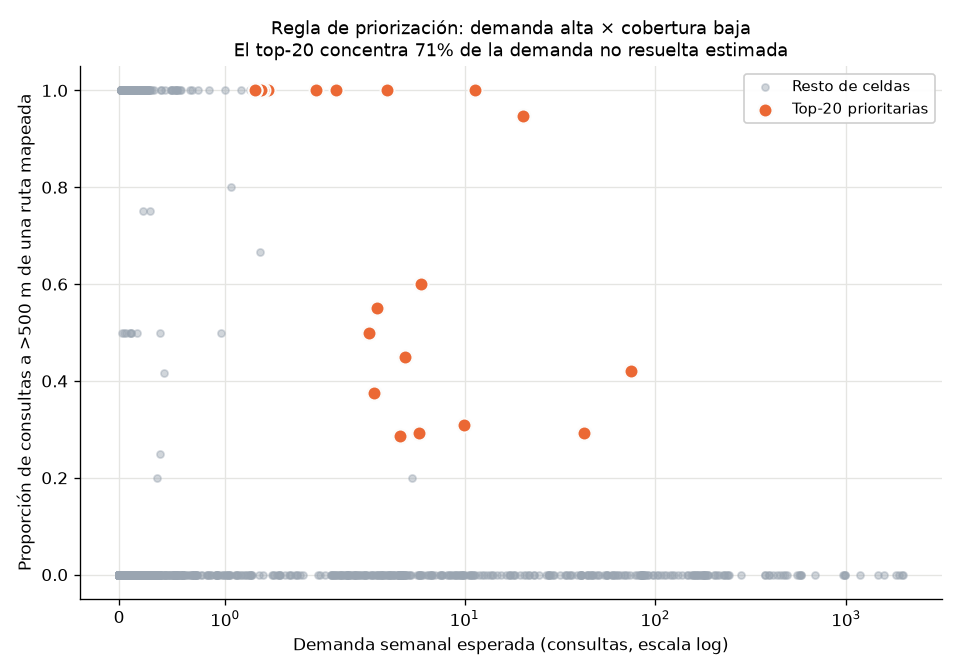
\includegraphics[width=0.75\textwidth]{imagenes/fig_priority_quadrants.png}
  \fuente{Elaboración propia, a partir de \var{27_priority_cells.py} ---
  \var{reports/05_deployment/03_priority_cells.md}.}
\end{figure}

El top-20 de celdas prioritarias concentra el \textbf{70,5~\%} de toda la demanda no resuelta
estimada del área metropolitana. Consistente con la figura, esas celdas \textbf{no son las de
mayor demanda absoluta}: son celdas de demanda baja o media (entre 1 y 74 consultas/semana)
mal cubiertas por el mapeo actual --la misma conclusión de H1 vista desde la decisión
operativa. Dieciocho de las veinte celdas coinciden entre usar Random Forest o la media móvil
como estimador de demanda, coherente con la refutación de la
sección~\ref{sec:sirve-para-priorizar}: el valor de esta tabla está en cruzar demanda con
cobertura, no en el estimador que produce la demanda.

\subsection{Monitoreo y reentrenamiento}
\label{sec:monitoreo}

Los umbrales de monitoreo se derivan de la distribución real de error y volumen de este
proyecto, no de valores convencionales.

\begin{table}[htbp]
  \centering
  \caption{Plan de monitoreo y reentrenamiento}
  \label{tab:monitoreo}
  \interlineadoSimple
  \begin{tabularx}{\textwidth}{@{}p{0.30\textwidth}p{0.16\textwidth}X@{}}
    \toprule
    \textbf{Métrica} & \textbf{Frecuencia} & \textbf{Umbral / acción} \\
    \midrule
    Volumen semanal total de consultas & Semanal & $<10.041$ consultas (30~\% de la mediana
    de las últimas 13 semanas no parciales) $\to$ marcar la semana como incompleta y
    excluirla del cálculo de \texttt{lag1} \\
    MAE semanal (predicción vs. real) & Semanal & $>11{,}64$ consultas (media $+\ 2\sigma$
    de las 6 semanas de prueba limpias) durante 2 semanas consecutivas $\to$ reentrenar antes
    del ciclo trimestral \\
    Actualización del feed GTFS & Semanal & Automática, ya implementada
    (\var{run_update_pipeline.py}) \\
    Reentrenamiento completo & Trimestral & Alineado con la ventana de 13 semanas de la
    validación cruzada (sección~\ref{sec:proceso-entrenamiento}) \\
    \bottomrule
  \end{tabularx}
  \fuente{Elaboración propia, a partir de \var{25_monitoring_plan.py} ---
  \var{reports/05_deployment/02_monitoring_plan.md}.}
\end{table}

El chequeo de completitud de datos existe \emph{porque} la sección~\ref{sec:semanas-parciales}
encontró el problema que previene: con este piso, las semanas 2024-W18 (909 consultas) y
2024-W23 (1.367 consultas) se habrían marcado automáticamente como incompletas en lugar de
descubrirse meses después durante el análisis de errores.

\subsection{Alcance del despliegue y trabajo pendiente}

No se despliega el servicio a un dominio público ni se automatiza el reentrenamiento con un
orquestador real (Airflow o un programador de tareas en un servidor productivo) --fuera del
alcance declarado de este trabajo (capítulo~\ref{cap:alcance}). Lo que se entrega en su lugar
es un prototipo funcional y verificable localmente, una arquitectura documentada que conecta
código ya existente, umbrales de monitoreo cuantificados a partir de los propios resultados
del proyecto, y una limitación operativa real --no hipotética-- descubierta al construir el
prototipo, con su mitigación propuesta. Antes de un uso productivo más allá de lo local
harían falta, como mínimo, autenticación, límites de tasa, un orquestador para el
reentrenamiento periódico y pruebas automatizadas de regresión sobre las métricas del modelo.

       % 7. Desarrollo (CRISP-DM)
% ============================================================
%  8. CONCLUSIONES Y RECOMENDACIONES   (guía, 2.8)
%  Regla explícita: las conclusiones deben derivarse de los
%  resultados y responder al objetivo general y a los específicos.
%  NO deben introducir información nueva no desarrollada antes.
% ============================================================
\chapter{Conclusiones y Recomendaciones}
\label{cap:conclusiones}

\section{Conclusiones}
\label{sec:conclusiones}

\subsection{Conclusión respecto del objetivo general}

La pregunta de investigación --en qué zonas del eje metropolitano de Cochabamba se
concentra la demanda de información de transporte no resuelta y qué características del
territorio se asocian con esa concentración (sección~\ref{sec:formulacion-problema})-- se
responde con evidencia convergente de tres análisis independientes
(sección~\ref{sec:interpretacion-resultados}): la brecha de cobertura centro-periferia es
real y estadísticamente significativa (H1, $p=6{,}1\times10^{-9}$); el gradiente espacial de
demanda es real y el modelo lo reproduce ($\rho=-0{,}615$ entre distancia al centro y
demanda observada); y el valor predictivo del modelo está concentrado exactamente en las
celdas de mayor demanda (H2), no distribuido de manera uniforme. El objetivo general
--construir un diagnóstico espacial de las brechas de información de transporte público y
derivar de él una lista priorizada de zonas de mapeo (sección~\ref{sec:objetivo-general})--
se cumple: el proyecto entrega tanto el diagnóstico (indicadores territoriales,
sección~\ref{sec:tabla-indicadores}, y contraste formal de la brecha, H1) como la lista
priorizada accionable (top-20 de celdas, sección~\ref{sec:priorizacion}), con evidencia de
que esta última no depende del modelo predictivo para ser útil.

A continuación se presentan las conclusiones correspondientes a cada objetivo específico.

\begin{enumerate}
  \item [OE1.] \textbf{Consolidar y auditar los archivos de consultas.} Se cumple
        íntegramente. Se consolidaron 1.927.675 registros de 85 exportaciones semanales sin
        pérdida ni duplicación silenciosa de filas (sección~\ref{sec:auditoria-esquema}),
        con las anomalías de esquema y codificación de seis archivos resueltas y
        documentadas, y la naturaleza de la variable \texttt{distancia} verificada
        empíricamente en lugar de asumida (sección~\ref{sec:validacion-distancia}). El
        resultado es un conjunto base donde cada fila excluida tiene un motivo registrado
        (tabla~\ref{tab:flujo-filtros}), cumpliendo el objetivo de trazabilidad completa
        entre el dato crudo y el dato modelado.
  \item [OE2.] \textbf{Caracterizar la demanda mediante análisis exploratorio
        espacio-temporal.} Se cumple. La demanda está fuertemente concentrada en el espacio
        (coeficiente de Gini de \textbf{0,934} en resolución 8, sección~\ref{sec:sensibilidad-h3})
        y decae con la distancia al centro; ambos patrones son estables ante cambios de
        resolución H3 --correlaciones de rangos superiores a 0,98 entre resoluciones
        adyacentes-- lo que descarta que sean un artefacto de la escala de agregación
        elegida (problema de la unidad de área modificable, capítulo~\ref{cap:marco-teorico}).
        En el tiempo, la demanda no es estacionaria y presenta un vacío estructural de siete
        semanas que condicionó la partición de entrenamiento y prueba
        (sección~\ref{sec:particion-cronologica}).
  \item [OE3.] \textbf{Construir indicadores territoriales por celda y semana.} Se cumple.
        La tabla de indicadores (sección~\ref{sec:tabla-indicadores}) integra demanda,
        cobertura GTFS, centralidad y composición temporal sobre 42.676 observaciones
        celda-semana, con el método de cálculo de cada variable documentado y nueve
        variables excluidas explícitamente por fuga de información
        (sección~\ref{sec:seleccion-algoritmos}). No se incorporaron Puntos de Interés de
        OpenStreetMap como variable de entorno urbano, decisión justificada por su
        cobertura desigual (capítulo~\ref{cap:alcance}) y retomada como recomendación más
        abajo.
  \item [OE4.] \textbf{Contrastar formalmente las hipótesis de brecha y de mejora
        predictiva.} Se cumple, con dos resultados que se refuerzan mutuamente. H1 se
        confirma: las celdas periféricas tienen una tasa de demanda no resuelta
        significativamente mayor que las centrales (Mann-Whitney,
        $p=6{,}1\times10^{-9}$, sección~\ref{sec:contraste-hipotesis}). H2 se confirma con
        matices: el test de Diebold-Mariano sobre la serie semanal no alcanza significancia
        por falta de potencia (8 puntos), pero el Wilcoxon pareado por celda sí
        ($p=0{,}033$), y la ventaja de Random Forest está concentrada en las celdas de
        mayor demanda --el segmento operativamente más relevante-- y no distribuida de
        forma uniforme.
  \item [OE5.] \textbf{Predecir demanda con modelos comparados contra líneas base.} Se
        cumple. Se compararon cuatro modelos de tres familias (Ridge, Lasso, Random Forest,
        XGBoost) bajo validación por ventanas deslizantes, nunca aleatoria
        (sección~\ref{sec:proceso-entrenamiento}). El hallazgo más informativo no fue qué
        modelo ``ganó'' en abstracto sino por qué los modelos lineales fallan: Ridge y
        Lasso extrapolan de forma inestable ante la tendencia de crecimiento sostenido,
        produciendo R\textsuperscript{2} fuertemente negativo en prueba pese a un ajuste
        razonable en entrenamiento --evidencia de que la relación entre demanda y
        condiciones territoriales no es lineal. Random Forest se seleccionó como modelo
        final con criterios explícitos, no por haber sido el primero ejecutado
        (sección~\ref{sec:seleccion-final}): MAE de prueba de \textbf{10,19} (o
        \textbf{5,91} excluyendo dos semanas de prueba que resultaron ser fragmentos de un
        solo día, sección~\ref{sec:semanas-parciales}), la evaluación más conservadora y la
        más representativa reportadas juntas, como corresponde cuando ninguna de las dos
        cifras por sí sola sería honesta.
  \item [OE6.] \textbf{Derivar una regla de priorización y contrastar el aporte del
        modelo.} Se cumple, con un resultado negativo declarado como tal. La regla de
        decisión --demanda esperada multiplicada por tasa de no cobertura-- produce un
        top-20 de celdas que concentra el 70,5~\% de la demanda no resuelta estimada
        (sección~\ref{sec:priorizacion}), y esas celdas no son las de mayor demanda
        absoluta sino zonas de demanda baja o media mal cubiertas --el mismo hallazgo de H1
        visto desde la decisión operativa. Pero el criterio preinscrito que evaluaría si el
        modelo predictivo mejora ese ordenamiento frente a una media móvil de 4 semanas
        \textbf{no se cumplió} (sección~\ref{sec:sirve-para-priorizar}): Random Forest no
        supera a la media móvil en ninguna de las seis semanas completas de prueba, en
        ninguna métrica de ordenamiento. Este resultado negativo, obtenido con un criterio
        declarado antes de observar los datos, es evidencia de rigor y no una falencia: para
        decidir qué celdas mapear a un horizonte de una semana no se justifica un modelo
        complejo, y la contribución del proyecto está en el pipeline reproducible, la
        caracterización territorial y el diagnóstico de cobertura, no en la superioridad de
        un estimador.
  \item [OE7.] \textbf{Proponer una arquitectura de actualización periódica.} Se cumple. Se
        construyó y se ejerció --no solo se documentó-- un prototipo real
        (\var{src/trufi_ds/api.py}) que sirve predicciones reconstruyendo las mismas
        variables usadas en entrenamiento, con ejemplos de consumo obtenidos de ejecuciones
        reales (sección~\ref{sec:despliegue}). Ejercitarlo expuso una limitación operativa
        real, no hipotética: la última semana del dataset es en sí misma una semana
        parcial, por lo que la primera predicción en producción heredaría la misma
        contaminación de rezago detectada en la evaluación. El plan de monitoreo deriva sus
        umbrales de la distribución real de error y volumen de este mismo proyecto,
        incluyendo un chequeo de completitud de datos que existe porque este proyecto
        encontró el problema que previene.
\end{enumerate}

\subsection{Limitaciones reconocidas}

Las limitaciones declaradas de antemano en el capítulo~\ref{cap:alcance} se sostienen, y se
completan con las que emergieron durante el desarrollo:

\begin{itemize}
  \item El feed GTFS usado para calcular cobertura tiene un período de validez declarado
        (2024-2026) posterior a buena parte de las consultas analizadas (desde 2022): la
        cobertura se mide contra el estado vigente del mapeo, no contra el estado que tenía
        en cada momento histórico.
  \item La cobertura se mide contra el trazado de la ruta (\texttt{shapes.txt}) y no contra
        las paradas (\texttt{stops.txt}), lo que mide accesibilidad a la línea de transporte
        y no al punto de abordaje efectivo, y por tanto sobreestima la cobertura tal como la
        percibe el usuario.
  \item La partición central/periferia usada en H1 se basa en la mediana de distancia al
        centro (15,49~km), un corte simple y documentado pero arbitrario, que no
        corresponde a ningún límite administrativo real.
  \item El test de Diebold-Mariano de H2 tiene solo ocho puntos, potencia insuficiente por
        construcción; su resultado no significativo no implica equivalencia entre modelos,
        y se complementó con el Wilcoxon pareado por celda por esa misma razón.
  \item Una celda ``sin cobertura'' puede tener servicio de transporte no mapeado en el
        GTFS de Trufi: la métrica localiza la brecha de \emph{información}, que es el
        objeto de este estudio, y no debe leerse como ausencia real de transporte.
  \item La demanda hereda el sesgo de adopción de la aplicación: zonas con menos usuarios de
        Trufi generan menos consultas aunque tengan mayor necesidad de transporte.
  \item El identificador de usuario es de nivel instalación, no de persona; una
        reinstalación genera un identificador nuevo y un dispositivo compartido produce el
        caso inverso.
  \item No se incorporaron Puntos de Interés de OpenStreetMap como variable de entorno
        urbano, ni un componente de segmentación por agrupamiento, por las razones
        declaradas en el capítulo~\ref{cap:alcance}.
  \item No existe una suite de pruebas automatizadas sobre el pipeline ni sobre las métricas
        del modelo, reconocida como la principal deuda técnica del proyecto.
\end{itemize}

Estas limitaciones acotan el alcance de las conclusiones anteriores sin invalidarlas: cada
hallazgo reportado --la brecha de cobertura, el gradiente espacial, la ventaja concentrada
del modelo, la refutación de su aporte al ordenamiento-- se sostiene dentro de estos límites
declarados, no a pesar de ocultarlos.

\section{Recomendaciones}
\label{sec:recomendaciones}

Las recomendaciones se derivan de los resultados obtenidos y de las limitaciones
identificadas; ninguna es genérica.

\begin{enumerate}
  \item [R1.] \textbf{Completar (\textit{backfill}) las semanas de datos parciales antes de
        cualquier despliegue real}: 2024-W18 y 2024-W23 con datos reales de esas semanas
        calendario completas (sección~\ref{sec:despliegue}); de lo contrario, la primera
        predicción en producción hereda el mismo artefacto que ya distorsionó la evaluación.
  \item [R2.] \textbf{Formalizar el chequeo de completitud de datos} (piso de 10.041
        consultas semanales, sección~\ref{sec:monitoreo}) como validación automática dentro
        del pipeline de actualización, no solo como umbral documentado --habría detectado
        el artefacto de semanas parciales en el momento en que ocurrió.
  \item [R3.] \textbf{Revisar la inestabilidad de extrapolación de los modelos lineales}
        antes de usarlos como referencia interpretable en producción: opciones concretas
        incluyen regresión cuantílica o un techo de extrapolación aprendido en vez del
        umbral fijo usado en este trabajo.
  \item [R4.] \textbf{Ampliar la validación de H1} más allá de la partición por mediana de
        distancia al centro, usando límites administrativos reales de periferia si se
        consigue una fuente confiable, en vez de un corte simple pero arbitrario.
  \item [R5.] \textbf{Aumentar la ventana de prueba} en un futuro ciclo de recolección de
        datos para dar más potencia al test de Diebold-Mariano, sin sacrificar datos de
        entrenamiento.
  \item [R6.] \textbf{Evaluar el aporte del modelo a horizontes de predicción mayores a una
        semana}: la refutación de la sección~\ref{sec:sirve-para-priorizar} vale
        específicamente para $h=1$ semana; a horizontes mayores la media móvil envejece y
        el modelo podría mostrar ventaja, pero esa prueba requiere reconstruir los rezagos
        a $h=2,3,4$ semanas y reentrenar, y queda pendiente.
  \item [R7.] \textbf{Incorporar Puntos de Interés de OpenStreetMap y un componente de
        segmentación territorial por agrupamiento} como extensiones del perfil de celda,
        considerados en el diseño original de este proyecto y descartados por razones de
        cobertura de datos y de alcance (capítulo~\ref{cap:alcance}), no por falta de
        valor potencial.
  \item [R8.] \textbf{Confirmar con el equipo de backend de Trufi App} si el cambio de
        esquema y codificación detectado en seis archivos, justo después del vacío de siete
        semanas, corresponde a un cambio real del proceso de exportación
        (sección~\ref{sec:auditoria-esquema}) --queda como pregunta abierta, nunca
        confirmada con la fuente.
  \item [R9.] \textbf{Antes de un despliegue productivo real}: agregar autenticación,
        límites de tasa, un orquestador para el reentrenamiento trimestral en vez de
        ejecución manual de scripts, y pruebas automatizadas de regresión sobre las
        métricas del modelo (sección~\ref{sec:despliegue}).
\end{enumerate}
     % 8. Conclusiones y Recomendaciones
% ============================================================
%  9. BIBLIOGRAFÍA Y ANEXOS   (guía, 2.9 y 3.6)
%  Bibliografía con biblatex + biber (Fase 4): estilo APA (2.6),
%  alfabética, sin numerar, sangría francesa, todo generado por
%  \printbibliography a partir de referencias.bib. Solo aparecen
%  las obras efectivamente citadas en el texto (\parencite en
%  secciones/03_problema.tex y 07_marco_teorico.tex); las demás
%  entradas de referencias.bib no citadas en el cuerpo quedan
%  fuera de la lista impresa, tal como exige "solo obras realmente
%  citadas" -- comportamiento nativo de biblatex, sin \nocite.
% ============================================================
\chapter{Bibliografía y Anexos}
\label{cap:bibliografia}

\section{Bibliografía}
\label{sec:bibliografia}

\printbibliography[heading=none]
% Nota interna sobre verificación de referencias y checklist de cierre:
% movidas a docs/notas_internas.md (defecto #9 — no van dentro del PDF).

\clearpage
\section{Anexos}
\label{sec:anexos}

Los anexos incorporan la evidencia técnica que respalda la monografía sin recargar el
cuerpo principal del documento.

\subsection{Anexo A. Diccionario de datos completo}
\label{anexo:diccionario-datos}

Ver tabla~\ref{tab:diccionario-datos} (sección~\ref{sec:diccionario-datos}) para el
diccionario completo del conjunto consolidado, incluyendo los campos de trazabilidad
(\var{source_file}, \var{source_batch}) añadidos durante la consolidación.

\subsection{Anexo B. Trazabilidad de notebooks y evidencias}
\label{anexo:trazabilidad-scripts}

Ver tabla~\ref{tab:trazabilidad-oe} (sección~\ref{sec:enlace-objetivos}) para la
correspondencia entre los objetivos específicos, los seis notebooks del pipeline y la
evidencia que produce cada uno. Estructura del repositorio del proyecto de datos:
\texttt{data/raw} (85 CSV de consultas, el feed GTFS y el archivo de Kontur, solo
lectura), \texttt{data/interim} (consultas limpias y tablas intermedias en formato Parquet),
\texttt{data/processed} (tabla de modelado por zona), \texttt{src} (funciones que llaman
los notebooks), \texttt{notebooks} (\var{01_eda} a \var{06_propuesta}) y
\texttt{resultados/<fase>} (tablas, figuras y \var{metricas.json} de cada fase).
     % 9. Bibliografía y Anexos

\end{document}
